%\documentclass[preprint,3p,times,twocolumn]{elsarticleUS}
\documentclass[review,3p,times]{elsarticleUS}
\usepackage{amssymb}
\usepackage{amsmath}
\usepackage{graphicx}
\usepackage{bm}
\usepackage{yhmath}
\usepackage{subfigure}
\usepackage{multirow}
\usepackage{color}
\usepackage{xcolor}
\usepackage{subdepth}
%\usepackage[nomarkers,lists]{endfloat}

\def\pp#1#2{\frac{\partial #1}{\partial #2}}

\biboptions{comma,sort&compress}

\journal{Fuel}

\makeatletter
\def\@author#1{\g@addto@macro\elsauthors{\normalsize%
    \def\baselinestretch{1}%
    \upshape\authorsep#1\unskip\textsuperscript{%
      \ifx\@fnmark\@empty\else\unskip\sep\@fnmark\let\sep=,\fi
      \ifx\@corref\@empty\else\unskip\sep\@corref\let\sep=,\fi
      }%
    \def\authorsep{\unskip,\space}%
    \global\let\@fnmark\@empty
    \global\let\@corref\@empty  %% Added
    \global\let\sep\@empty}%
    \@eadauthor={#1}
}
\makeatother

\begin{document}

\begin{frontmatter}

\title{Sooting Limits of Nonpremixed $n$-Heptane, $n$-Butanol, and Methyl Butanoate Flames: Experimental Determination and Mechanistic Analysis}

\author{Sili~Deng\corref{cor}}
\cortext[cor]{Corresponding Author: silideng@princeton.edu}
\author{Jeremy A.~Koch}
\author{Michael E.~Mueller}
\author{Chung K.~Law}

\address{Department of Mechanical and Aerospace Engineering, Princeton University, Princeton, NJ 08544, USA}


\begin{abstract}
The sooting limits of nonpremixed $n$-heptane, $n$-butanol, and methyl butanoate flames were determined experimentally in a liquid pool stagnation-flow configuration.  In addition, complementary simulations with detailed polycyclic aromatic hydrocarbon (PAH) chemistry and a detailed soot model, based on the Hybrid Method of Moments (HMOM), were performed and compared with the experimental critical strain rates for the sooting flames.  Argon dilution was used to keep the thermal environment for the three fuel cases nearly the same to elucidate the chemical effects.  Both experiment and simulation showed that $n$-heptane and $n$-butanol had similar sooting characteristics, while methyl butanoate had the least sooting propensity.  Further sensitivity and reaction path analysis demonstrates that the three fuels share similar PAH chemical pathways, and C$_5$ and C$_6$ ring formation from the intermediate chain species is found to be the rate-limiting step.  The differences in sooting propensity lie in the fuel breakdown processes.  Specifically, the oxygen bounded in $n$-butanol does not reduce soot precursor concentrations but is primarily involved in intramolecular water elimination reactions. On the contrary, the fuel bound oxygen in methyl butanoate shortens the carbon chain of the soot precursors and promotes their oxidation, which reduces the total carbon available for soot formation. 
\end{abstract}

\begin{keyword} 
Soot \sep Nonpremixed stagnation-flow flame \sep
Hybrid Method of Moments \sep $n$-Butanol \sep Methyl butanoate
\end{keyword}

\end{frontmatter}

%\clearpage % For word count
\section{Introduction}

The utilization of biofuels, which are potential partial replacements for liquid fuels derived from fossil fuels, is garnering wide attention not only because these fuels are renewable, locally producible, and carbon neutral~\cite{liu11} but also due to their potential positive impacts on particulate matter (PM) emission control. Biofuels, including bioalcohols and biodiesels, mainly consist of oxygenated hydrocarbons, such as ethers, alcohols, and esters. When used as additives in conventional diesel fuels, PM emissions have been found to decrease as oxygenated additive concentrations increase~\cite{graboski98}. 

However, the precise role of oxygenated additives on soot emission reduction has not yet come to a scientific consensus. For example, Frijters and Baert~\cite{frijters06} attributed the PM reduction to the fuel oxygen content, which reduced the local equivalence ratio and, by implication, the flame temperature.  However, even with the same oxygen content, the oxygenates had different efficiencies in soot precursor reduction, as Westbrook \emph{et al.}~\cite{westbrook06} found through simulations of premixed $n$-heptane and oxygenates flames.  Furthermore, Pepiot \emph{et al.}~\cite{pepiot08} proposed a structural group contribution approach to interpret diesel engine experimental data and quantify the soot reduction tendency of oxygenated fuels.  As noted by the authors, the aromatics contained in the conventional diesel fuels have very strong sooting tendencies, which are moderated through substitution by the clean-burning oxygenated additives; this replacement effect should be identified and quantified to reveal the role of the oxygen moieties. 

Conversely, a number of studies show that oxygenated fuels do not necessarily have lower sooting tendencies than regular hydrocarbons.  McEnally and Pfefferle~\cite{mcenally05,mcenally11} found that butanol isomer doped methane co-flow diffusion flames produce more soot than the undoped ones.  As only $1000$ ppm of each test compound was added to the methane stream, the study was able to identify the direct chemical effects of the addtives.  It was subsequently found that the effect of carbon chain length on soot formation is often larger than the direct chemical effects of oxygen and branches in the carbon chain promote soot formation.  Similar conclusions were reached by Camacho \emph{et al.}~\cite{camacho13} by probing the evolution of the detailed particle size distribution function in a set of laminar premixed flames of $n$- and $i$-butane/butanol with fixed C/O ratio and maximum temperature. 

To further explore the sooting characteristics of oxygenated fuels and understand the chemical pathways for soot formation processes, additional well-controlled fundamental experiments and detailed chemical kinetic analyses need to be performed.  In particular, it is recognized that, besides the thermal and replacement effects of oxygenated additives, the residence times of soot precursors are also expected to influence the sooting propensities~\cite{tsuji71} since soot formation is a kinetically controlled process~\cite{vandsburger85}.  Therefore, the present experimental and computational study focuses on the sooting limits (a residence time effect) of three neat liquid diesel/biofuel components, specifically, $n$-heptane, $n$-butanol, and methyl butanoate, in a nonpremixed stagnation-flow. A combined chemical kinetic model with detailed polycyclic aromatic hydrocarbon (PAH) chemistry is constructed to investigate the important pathways of soot formation with these three fuels.

This choice of the target fuels is motivated by both practical and scientific concerns. First, butanol has more diverse non-food sources of supply than ethanol, which has been derived primarily from corn. Second, methyl butanoate is chosen not only because it is a typical biodiesel surrogate but also due to the availability of detailed chemical kinetic models. Third and most important, the boiling points of $n$-butanol and methyl butanoate are $391$ K and $375$ K, respectively, which are very close to that of $n$-heptane ($372$ K). This similarity in the vaporization characteristics enables similar fuel vapor concentrations above the stagnation liquid pool and assures similar rates of supply of the vaporized fuel to the flame region.


\section{Experimental Methodology}
\label{sec:2}

The sooting limits of nonpremixed model diesel/biofuel components, in terms of the critical strain rate (CSR) at which soot inception starts to happen when the residence time, which is the inverse of the strain rate, is further increased, were measured at atmospheric pressure in a liquid pool stagnation-flow configuration. An unheated oxidizer stream impinged against the liquid fuel pool, and flames were established by spark ignition. Coflowing nitrogen was utilized as the shielding gas to minimize the disturbance from the surroundings.  With the $20$ mm nozzle and pool diameter, the separation distance between the oxidizer nozzle and liquid pool was maintained at $13$ mm to assure a well-characterized stagnation flow and also to enable better measurement of the velocity field by Laser Doppler Velocimetry (LDV).  The schematic of the liquid pool stagnation-flow apparatus is shown in Fig.~\ref{fig:setup}, and details about the auxiliary system can be found elsewhere~\cite{liu10}.

Due to the oxygen content in $n$-butanol and methyl butanoate, their flame temperatures are lower than $n$-heptane. Since soot formation is highly sensitive to temperature~\cite{wang11}, this thermal effect has to be eliminated to elucidate the chemical effects. In the present study, $n$-butanol and methyl butanoate flame temperatures were increased to be the same as $n$-heptane by replacing a portion of the nitrogen in the oxidizer stream with argon, which is the same approach taken by Axelbaum, Law, and co-workers~\cite{du89,du91,axelbaum91}. The amount of nitrogen replacement was calculated with CHEMKIN's equilibrium solver EQUIL~\cite{chemkin} for stoichiometric fuel/oxidizer mixtures, and the diluent concentrations are summarized in Table.~\ref{table:exp_condition}.  Although the replacement was calculated based on premixed stoichiometric mixtures, the thermal environment of all three fuels cases under the same strain rate and oxygen mole fraction in the stagnation-flow configuration is nearly the same, according to the simulations, which will be discussed in detail in Sec.~\ref{sec:4}.  Liquid $n$-heptane, $n$-butanol, and methyl butanoate were fed to the liquid pool by a syringe pump at room temperature.

\begin{figure}[t]
  \centering
  \scriptsize
%  \vspace{-0.1in}
  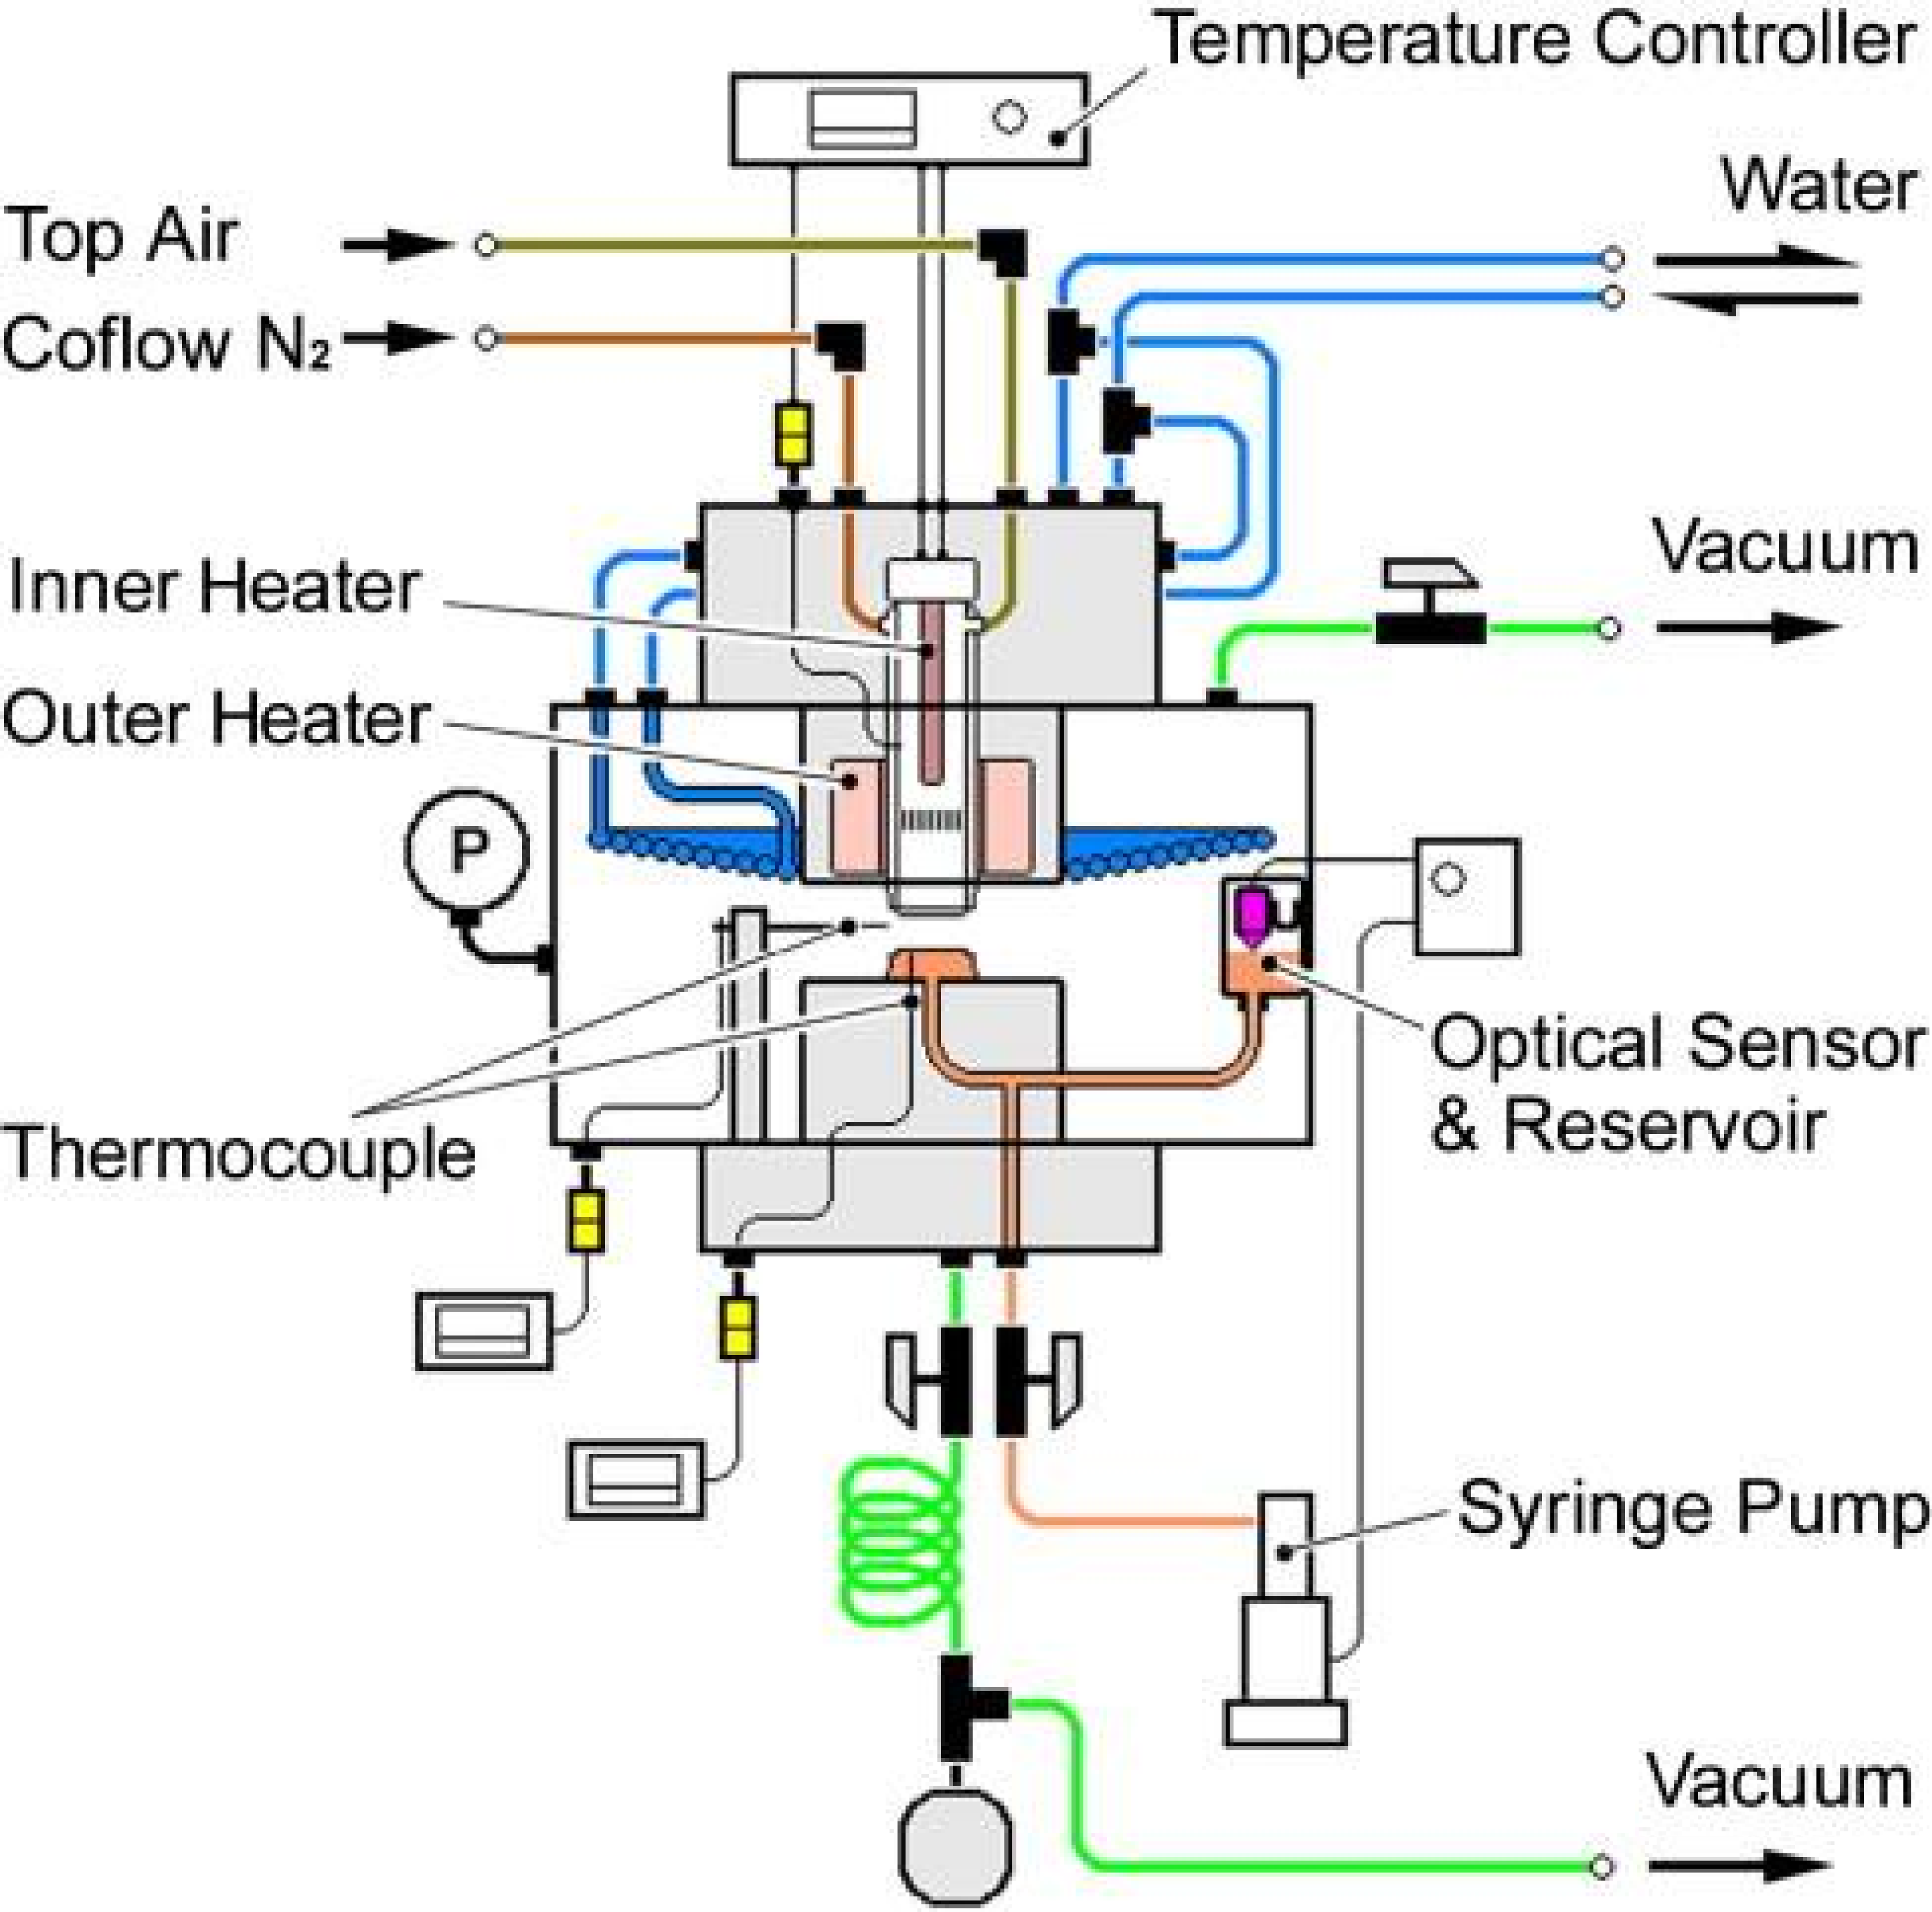
\includegraphics[width=0.4\textwidth]{Setup.png}
  \normalsize
%  \vspace{-0.1in}
  \caption{Schematic of the liquid pool stagnation-flow apparatus~\cite{liu10}.  The heating system was not activated in the current study.}
  \label{fig:setup}
\end{figure}



%\begin{table*}
%  \caption{Oxidizer stream composition in mole fractions.}
%  \label{table:exp_condition}
%  \centering
%  \resizebox{0.8\textwidth}{!}{
%  \begin{tabular}{ll*{10}{c}}
%    \hline
%     & \multicolumn{10}{c}{$O_2$} \\
%    \cline{3-12}
%     &  & $0.1950$ & $0.1975$ & $0.2000$ & $0.2025$ & $0.2050$ & $0.2075$ & $0.2100$ & $0.2150$ & $0.2200$ & $0.2250$ \\
%    \hline
%%    $n-C_7H_{16}$ & $N_2$ &  $0.8200$ & $0.8150$ & $0.8125$ & $0.8100$ & $0.8075$ & $0.8050$ &  & $0.8000$ \\
    %%    \hline
    %%    \multirow{2}{*}{$n-C_4H_9OH$} & $N_2$ &  &   &  &  &  & $0.7718$ & $0.7679$ & $0.7640$ & $0.7600$ & $0.7560$ & $0.7521$ \\
%    $n-C_4H_9OH$ & $N_2$ & $0.7718$ & $0.7679$ & $0.7640$ & $0.7600$ & $0.7560$ & $0.7521$ \\
%                 & $Ar$ & $0.0332$ & $0.0346$ & $0.0360$ & $0.0375$ & $0.0390$ & $0.0404$ \\
    %%    \hline
    %%    \multirow{2}{*}{$C_5H_{10}O_2$} & $N_2$ & & & & & & & & & & $0.7119$ & & $0.7017$ & $0.6915$ & $0.6811$ & $0.6707$ \\
 %   $C_5H_{10}O_2$ & $N_2$ & & & & & $0.7119$ &$0.7068$ & $0.7017$ & $0.6915$ & $0.6811$ & $0.6707$ \\
 %                & $Ar$ & & & & & $0.0831$ &$0.0857$ & $0.0883$ & $0.0935$ & $0.0989$ & $0.1043$ \\ 
 %   \hline
 % \end{tabular}
%}
%\end{table*}

\begin{table*}
  \caption{Oxidizer stream composition in mole fractions.}
  \label{table:exp_condition}
  \centering
  \resizebox{0.8\textwidth}{!}{
  \begin{tabular}{ll*{8}{c}}
    \hline
     & \multicolumn{8}{c}{$O_2$} \\
    \cline{3-10}
     &  & $0.2000$ & $0.2025$ & $0.2050$ & $0.2075$ & $0.2100$ & $0.2150$ & $0.2200$ & $0.2250$ \\
    \hline
    $n-C_4H_9OH$ & $N_2$ & $0.7640$ & $0.7600$ & $0.7560$ & $0.7521$ \\
                 & $Ar$ & $0.0360$ & $0.0375$ & $0.0390$ & $0.0404$ \\
    %%    \hline
    %%    \multirow{2}{*}{$C_5H_{10}O_2$} & $N_2$ & & & & & & & & & & $0.7119$ & & $0.7017$ & $0.6915$ & $0.6811$ & $0.6707$ \\
    $C_5H_{10}O_2$ & $N_2$ & & & $0.7119$ & & $0.7017$ & $0.6915$ & $0.6811$ & $0.6707$ \\
                 & $Ar$ & & & $0.0831$ & & $0.0883$ & $0.0935$ & $0.0989$ & $0.1043$ \\ 
    \hline
  \end{tabular}
}
\end{table*}


Soot detection was based on luminosity observations with a Nikon D700 camera, for Du \emph{et al.}~\cite{du89} found that such measurements agreed well with light scattering detection and were a convenient indicator of the presence of soot particles. The experimental procedure to identify the sooting limit is briefly summarized here. First, the oxidizer component flow rates were set, and a non-sooting blue flame was established. Then, the bypass valve placed upstream of the oxidizer nozzle was slowly adjusted to divert oxidizer out of the system, effectively reducing the velocity of the stream and, consequently, the strain rate. The residence time was further increased until yellow luminosity began to appear on the fuel rich side of the flame. A standard single-component LDV measurement was performed along the axial centerline under this threshold flow condition, and the local strain rate was determined as the axial velocity gradient upstream of the flame~\cite{du89}. Following this procedure, the sooting limits for the three fuels with different oxygen concentrations in the oxidizer streams were identified.  Although this luminosity measurement was not quantified, the CSR measurements were found to be repeatable.

\section{Computational Methodology}

The liquid pool stagnation-flow flames were simulated with the FlameMaster code~\cite{flamemaster}, including detailed PAH chemistry and a detailed soot model. The boundary conditions on the fuel side were specified following Bui-Pham \emph{et al.}~\cite{buipham91}. In brief, the Antoine equation~\cite{polingbook} was used to close the boundary value problem by relating the liquid pool surface temperature and vapor pressure, yielding a relationship for the fuel mole fraction at the surface. As in the experiment, the local strain rate was determined as the gradient of the velocity profile on the oxidizer side, ahead of the flame. 

Furthermore, since the luminosity observations cannot be simulated directly, the computational CSRs were determined based on an alternative metric, and a critical value of this metric was chosen to match the experimental results of $n$-heptane at larger $X_{O_2}$ cases and was kept fixed for all other cases.  The global domain-integrated soot volume fraction ($f_V$), the temperature-weighted global domain-integrated soot volume fraction ($f_V*$T$^4$), and the maxima of the corresponding single-point values were considered as potential metrics.  However, the qualitative trends presented in the next section were found to be insensitive to the choice of the threshold value or determination metrics that were explored.  Therefore, the global domain-integrated $f_V$ (m$^3$/m$^2$) were chosen as the metric for computational determination of CSRs in the following sections.

\subsection{Chemical Model} 

A detailed chemical model including PAH chemistry was constructed from three well validated models corresponding to the fuels of interest. A mechanism with PAH chemistry of engine relevant fuels was developed by Blanquart, Pitsch, and co-workers~\cite{blanquart09b,narayanaswamy10}. This mechanism has been validated extensively against experimental measurements of ignition delay times, laminar burning velocities, and species profiles in both premixed and nonpremixed flames over a large range of equivalence ratios and pressures for small hydrocarbons, C$_3$ and C$_4$ species, (substituted) aromatics, $n$-heptane, and iso-octane. Of particular interest to this work, the mechanism was validated in $n$-heptane nonpremixed flames against the measurements of Berta \emph{et al.}~\cite{berta06}. In the present study, this mechanism was adopted as the base mechanism with PAH chemistry. Reduced oxidation/pyrolysis chemistry of $n$-butanol and methyl butanoate kinetic models was adopted from Liu \emph{et al.}~\cite{liu11} and combined with the base mechanism.  These models were reduced from the detailed mechanisms of Sarathy \emph{et al.}~\cite{sarathy09} and Ga\"il \emph{et al.}~\cite{gail08}, respectively. Details about the mechanism reduction, validation, and reduced mechanisms can be found in Liu \emph{et al.}~\cite{liu11}.  All the common reactions among the base mechanism and the addtional mechanisms were retained from the base mechanism to maintain compatibility with the PAH mechanism. The thermal and transport data of the species that appeared only in the $n$-butanol and methyl butanoate mechanism were taken from these latter works, and species in common were taken from the base mechanism. The combined mechanism consists of $220$ species and $2259$ forward and backward reactions; none of the reaction rate parameters were adjusted in the combined mechanism.

The combined mechanism  was validated against laminar flame speed measurements~\cite{liu11} and compared with the predictions by the original mechanisms; results of this validation are shown in Fig.~\ref{fig:validation}.  As no difference was found between the validation results calculated by the combined and the original $n$-heptane mechanism, $n$-heptane laminar speed validation is not included in Fig.~\ref{fig:validation} and can be found in the referenced works~\cite{blanquart09b,narayanaswamy10}.  The differences between the combined mechanism and the original mechanism for $n$-butanol and methyl butanoate are attributed to the differences in the base chemistry, with the combined mechanism generally giving improved agreement with the experimental measurements.  

In addition, the combined mechanism was further validated against extinction strain rate (ESR) measurements in the nonpremixed liquid pool stagnation-flow system, as shown in Fig.~\ref{fig:validation-ESR}.  The computational ESR for $n$-heptane and methyl butanoate were compared with the experimental studies of Seshadri and co-workers~\cite{seshadri08,niemann10}, and details about the experimental procedure and conditions can be found therein.  These measurements were augmented with our own measurements of ESR for $n$-butanol with the same apparatus presented in the previous section.  The same experimental procedure as Seshadri and co-workers was adopted, except that the ESR was defined by the local strain rate rather than the global one, the former being the fundamentally more relevant quantity.  In all cases, the experimental measurements and simulation results were compared based on the same definition of the strain rate.  However, as demonstrated in Liu \emph{et al.}~\cite{liu11b}, deteminations based on a given definition are consistent.  As shown in Fig.~\ref{fig:validation-ESR}, computational ESRs for $n$-heptane and methyl butanoate agree well with the experimental measurements and are slightly overpredicted for $n$-butanol.  

\begin{figure}[t]
  \centering
  \scriptsize
%  \vspace{-0.1in}
  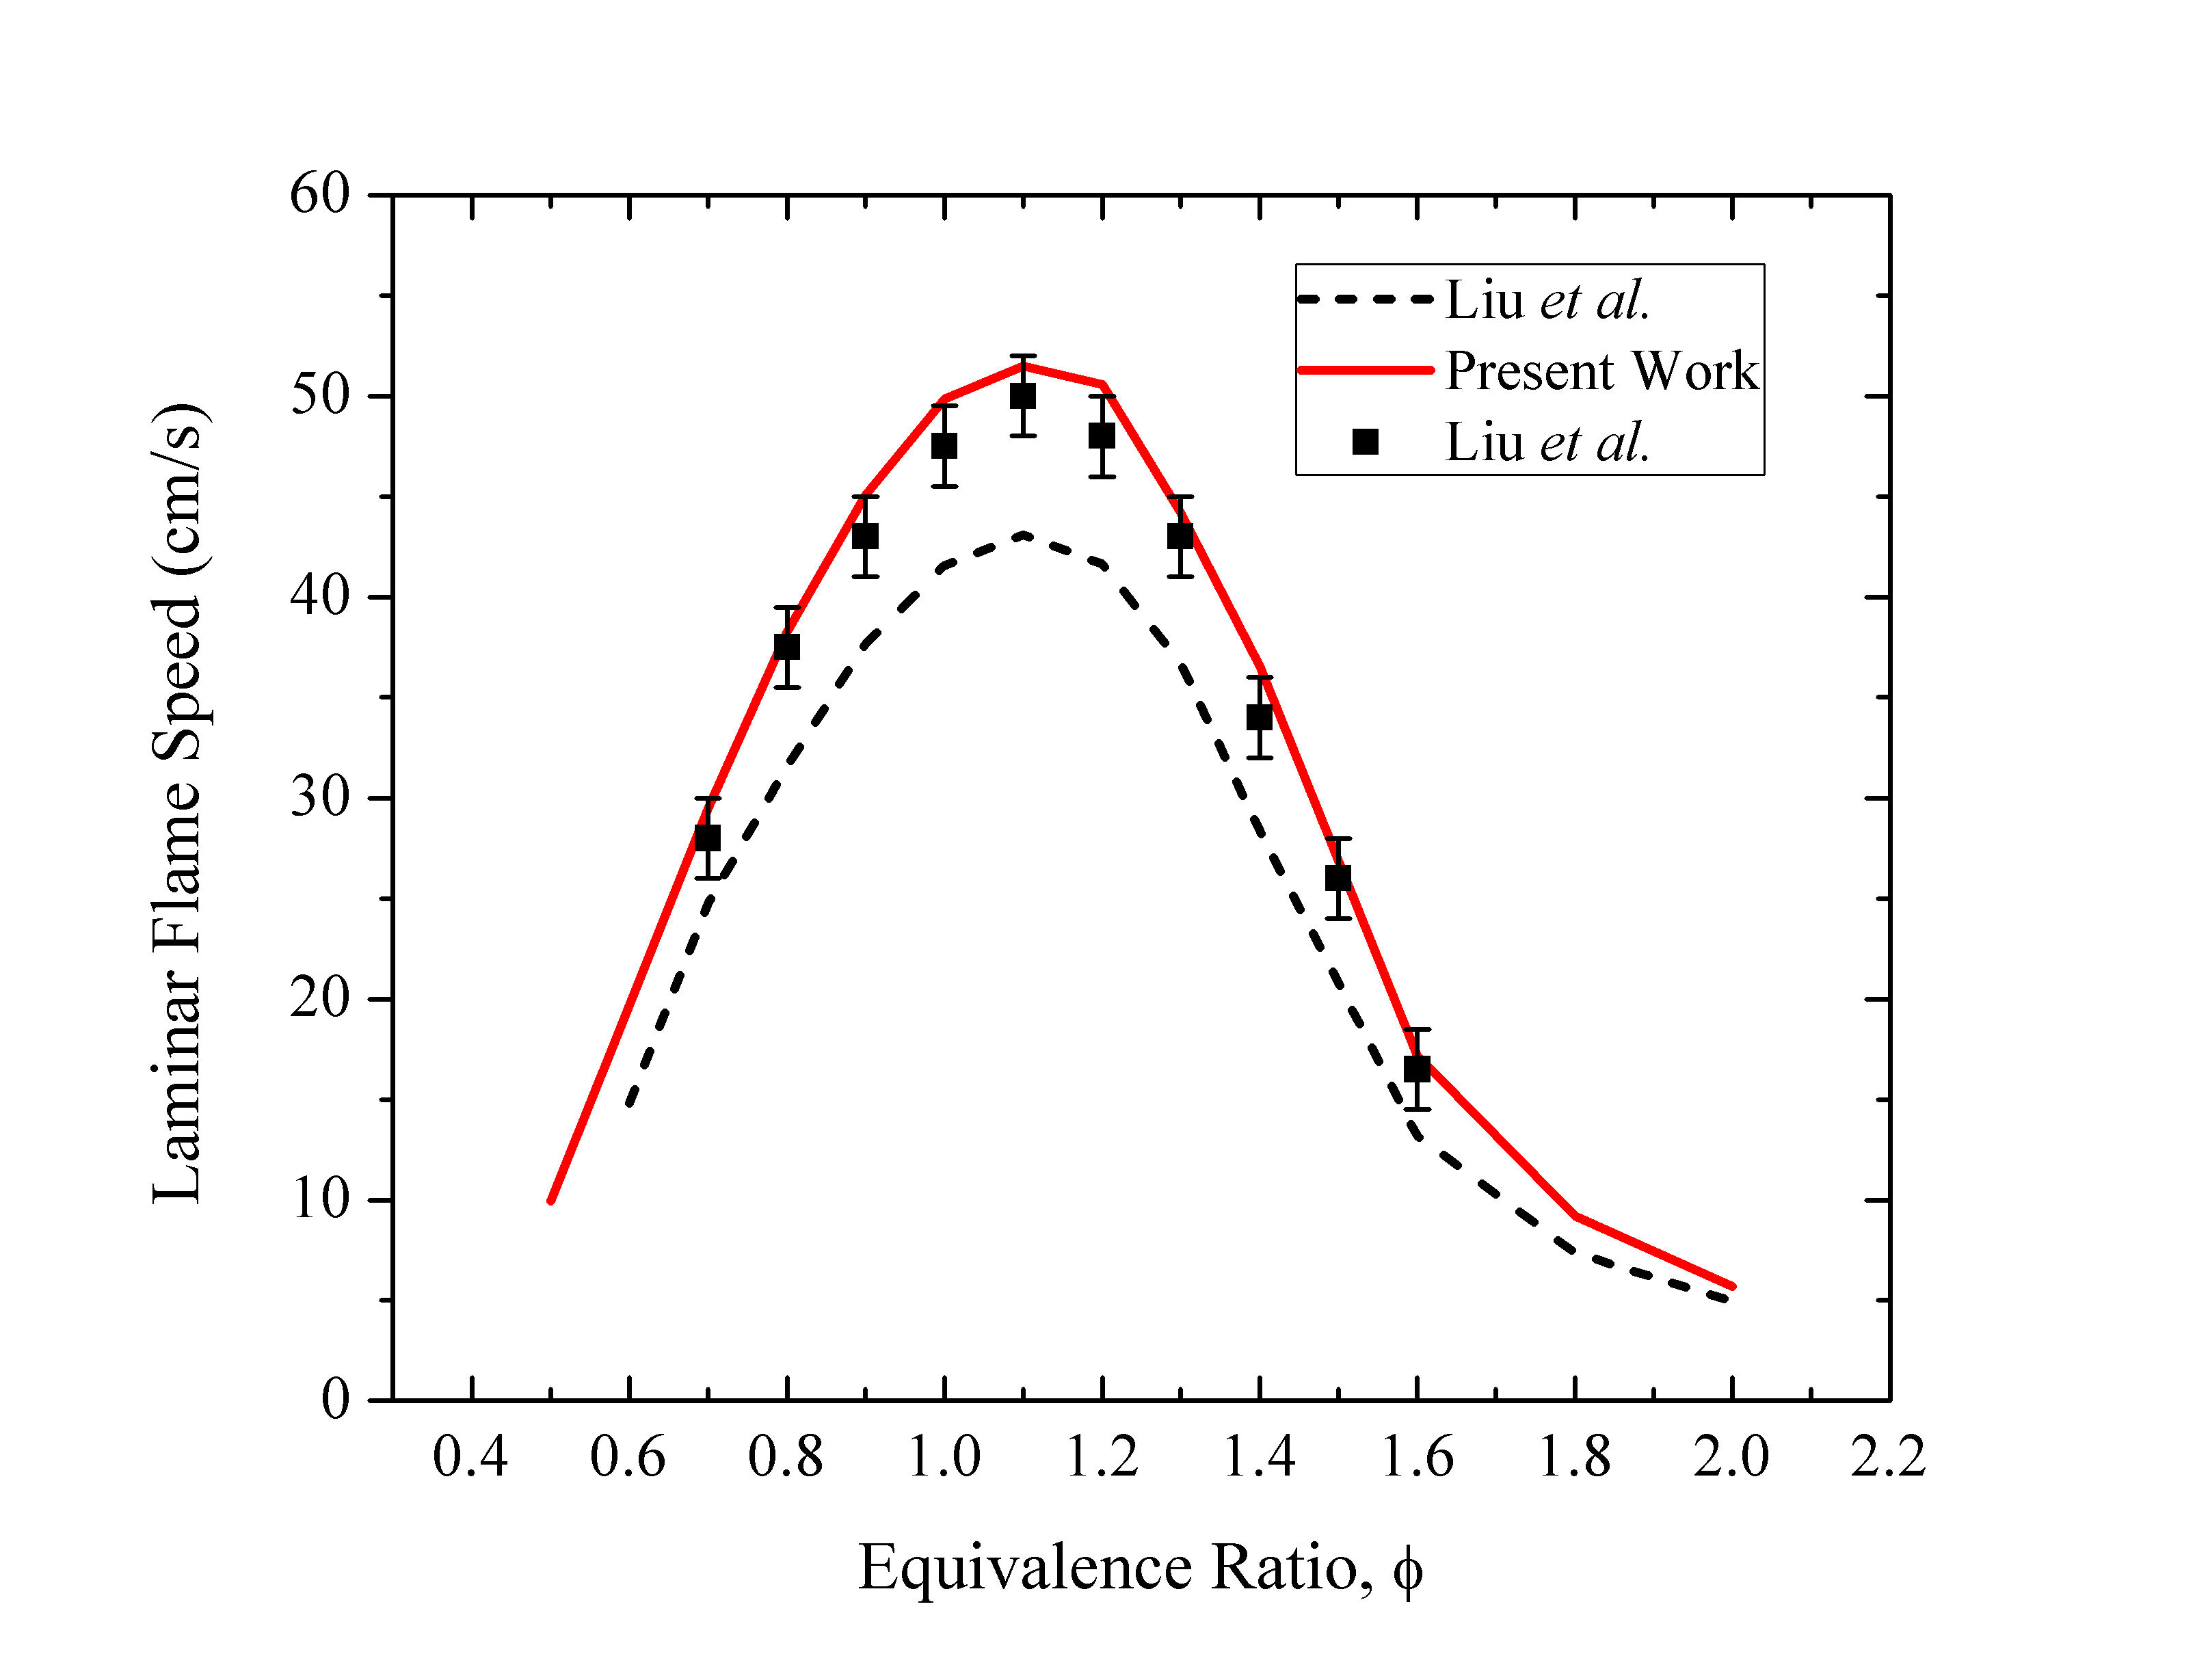
\includegraphics[trim=4mm 8mm 30mm 20mm, clip=true, width=0.4\textwidth]{NB.png}
  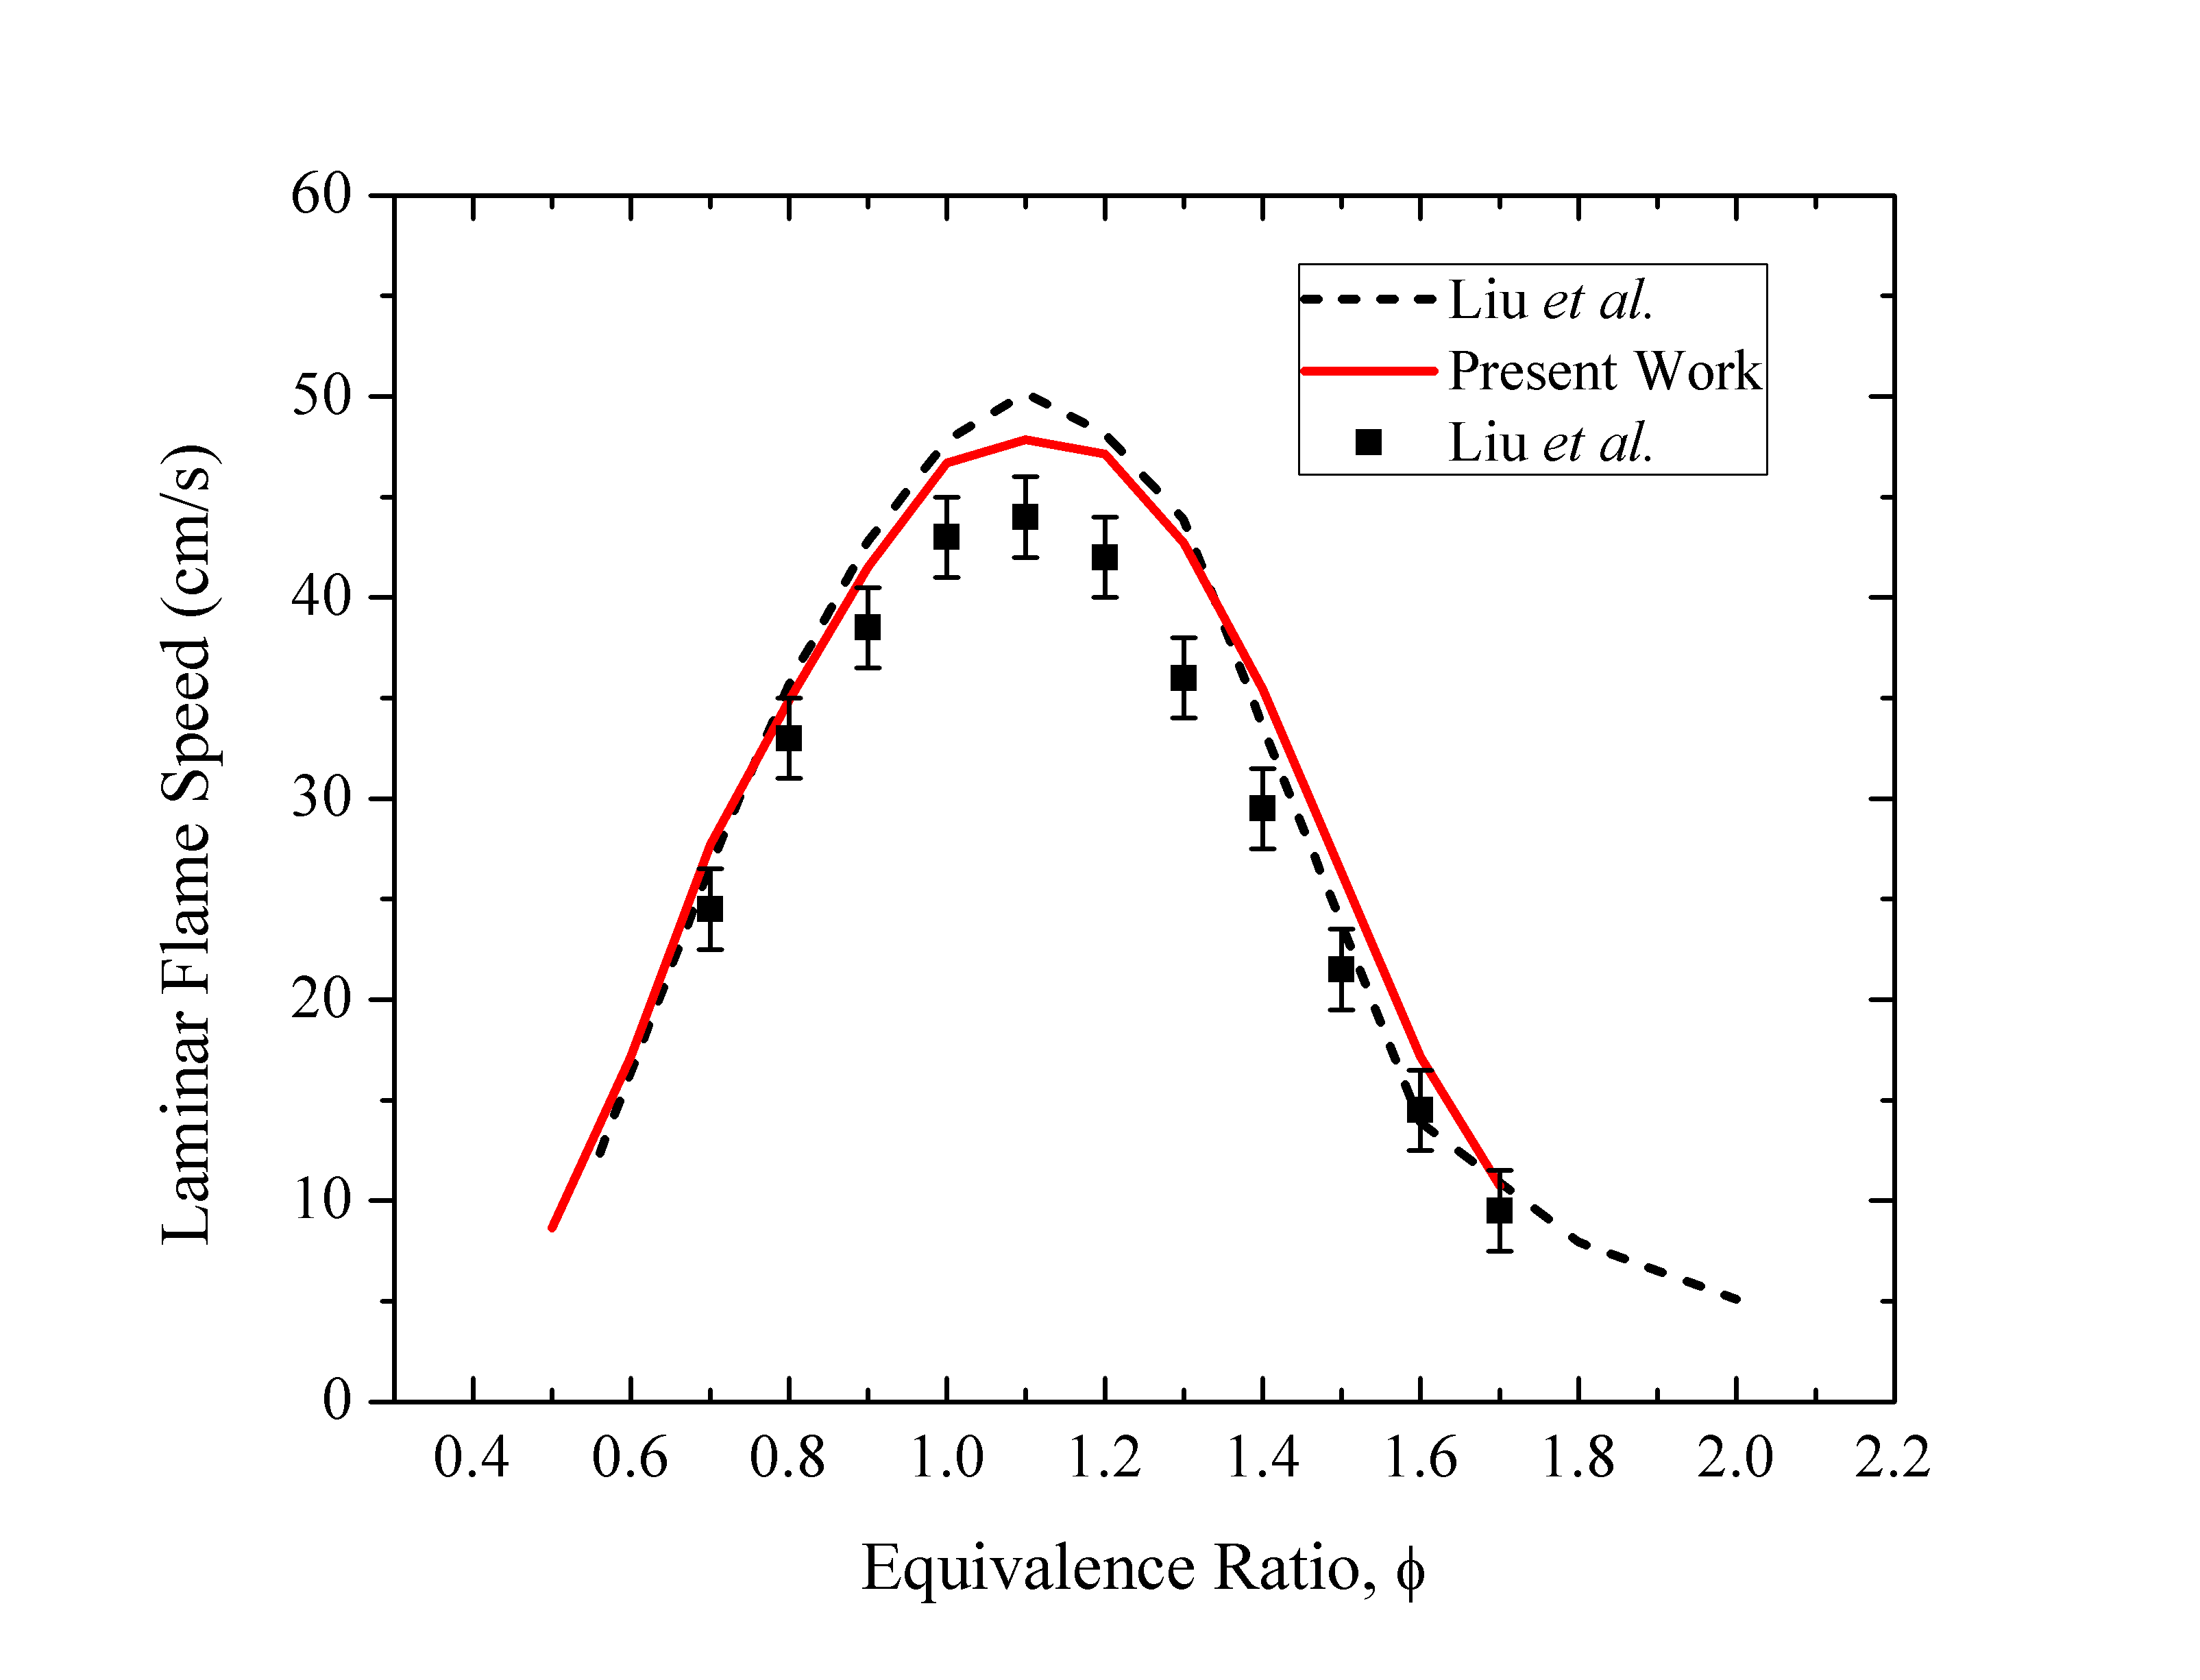
\includegraphics[trim=4mm 8mm 30mm 20mm, clip=true, width=0.4\textwidth]{MB.png}
  \normalsize
  \vspace{-0.1in}
  \caption{Mechanism validation of $n$-butanol (left) and methyl butanoate (right) laminar flame speeds, against the experimental (symbols) and computational (dotted lines) results from Liu \emph{et al.}~\cite{liu11}. $P=1$ atm and $T=353$ K.}
  \label{fig:validation}
\end{figure}

\begin{figure}[t]
  \centering
  \scriptsize
%  \vspace{-0.1in}
  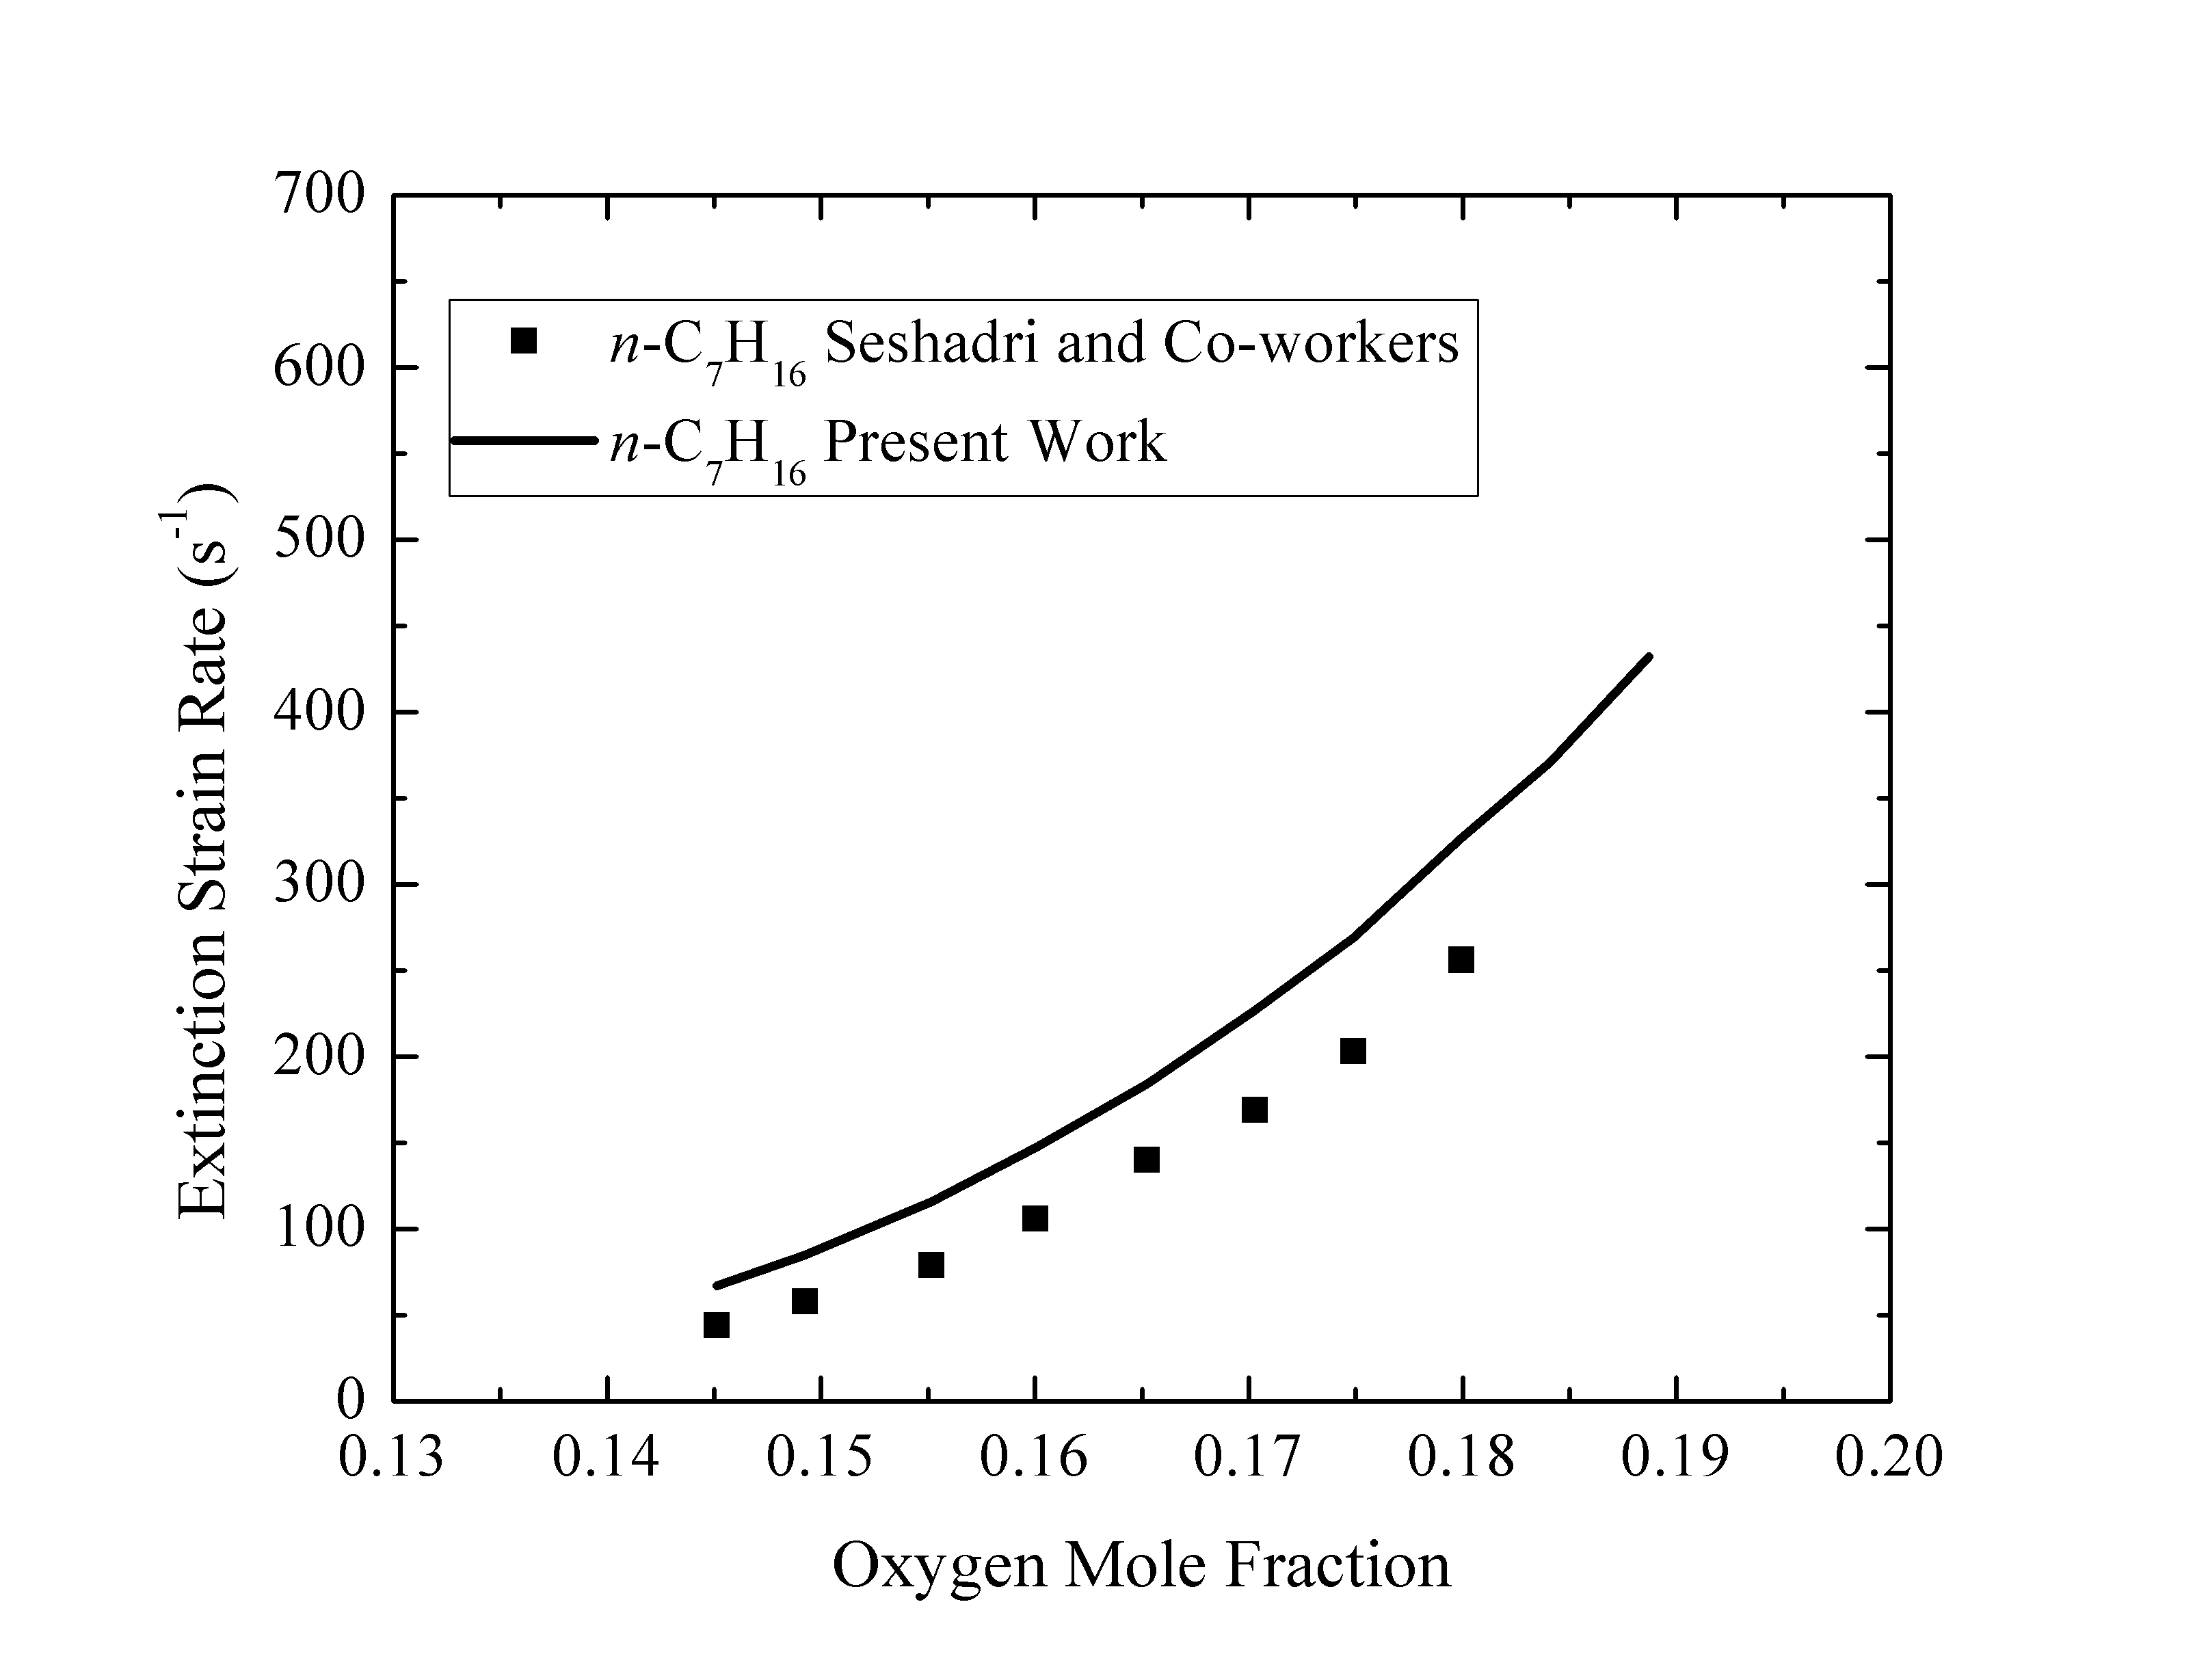
\includegraphics[trim=4mm 8mm 30mm 20mm, clip=true, width=0.4\textwidth]{NH-ESR.png}
  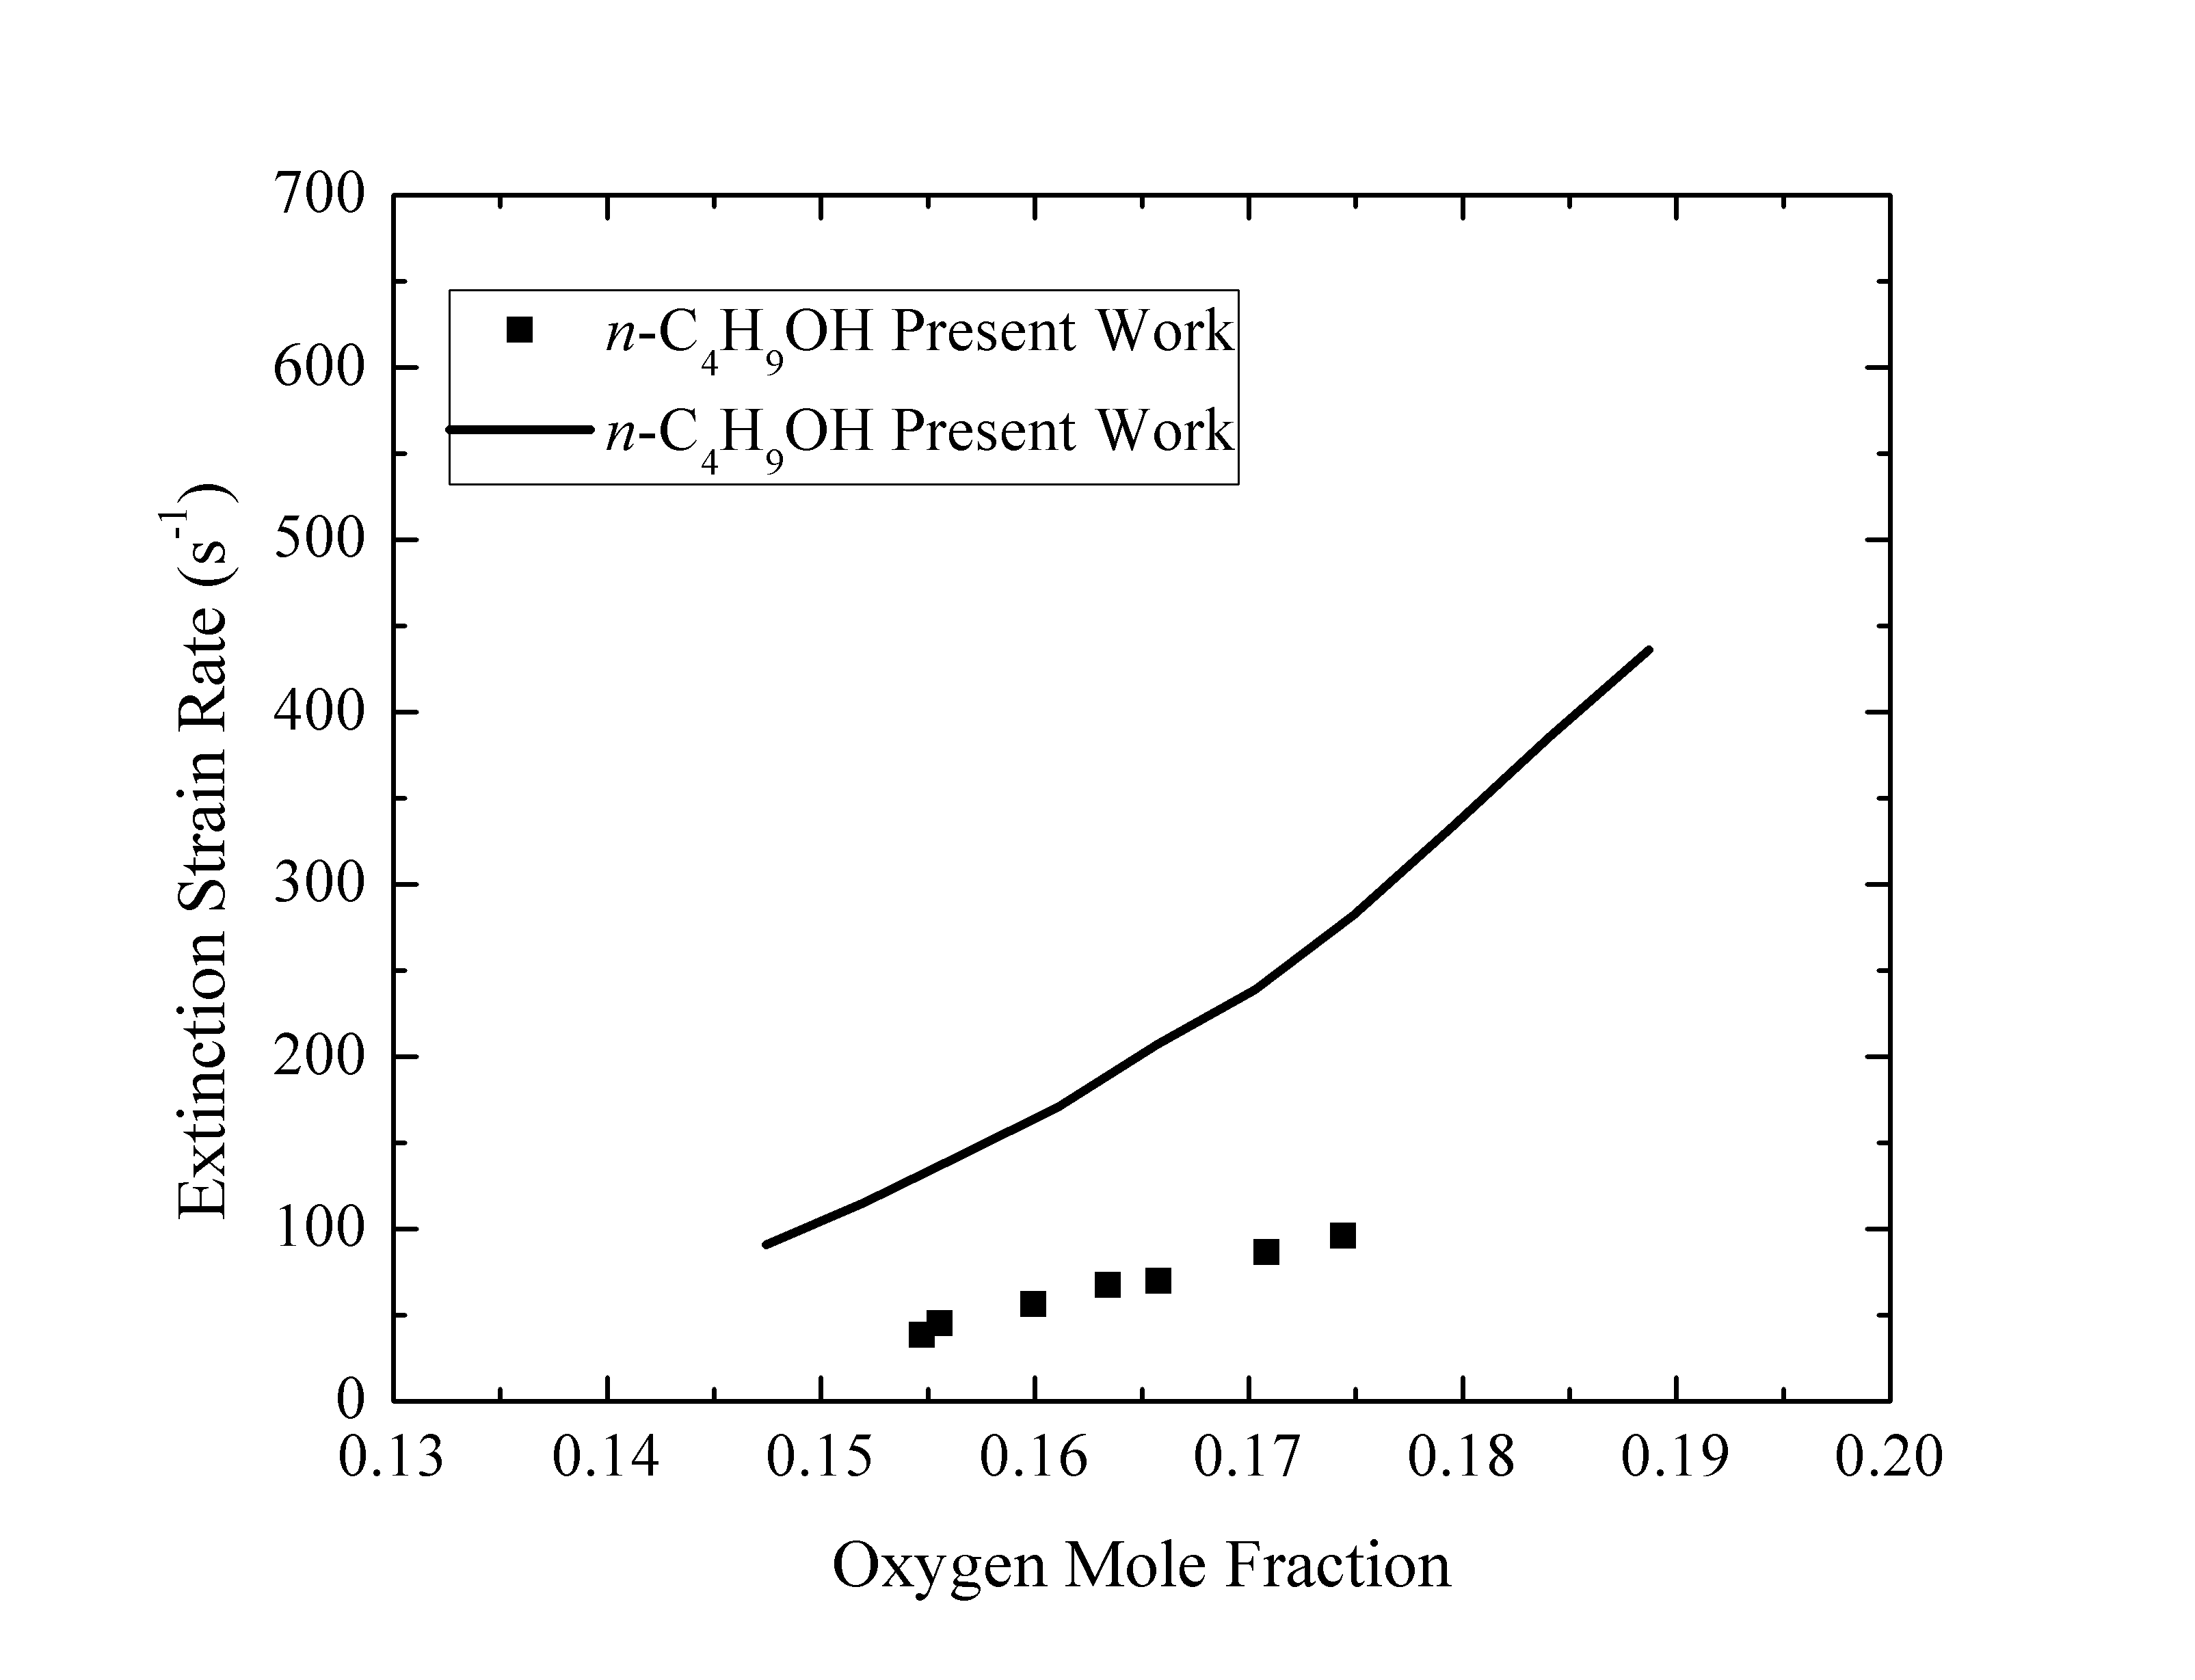
\includegraphics[trim=4mm 8mm 30mm 20mm, clip=true, width=0.4\textwidth]{NB-ESR.png}\\
   \vspace{0.5in}
  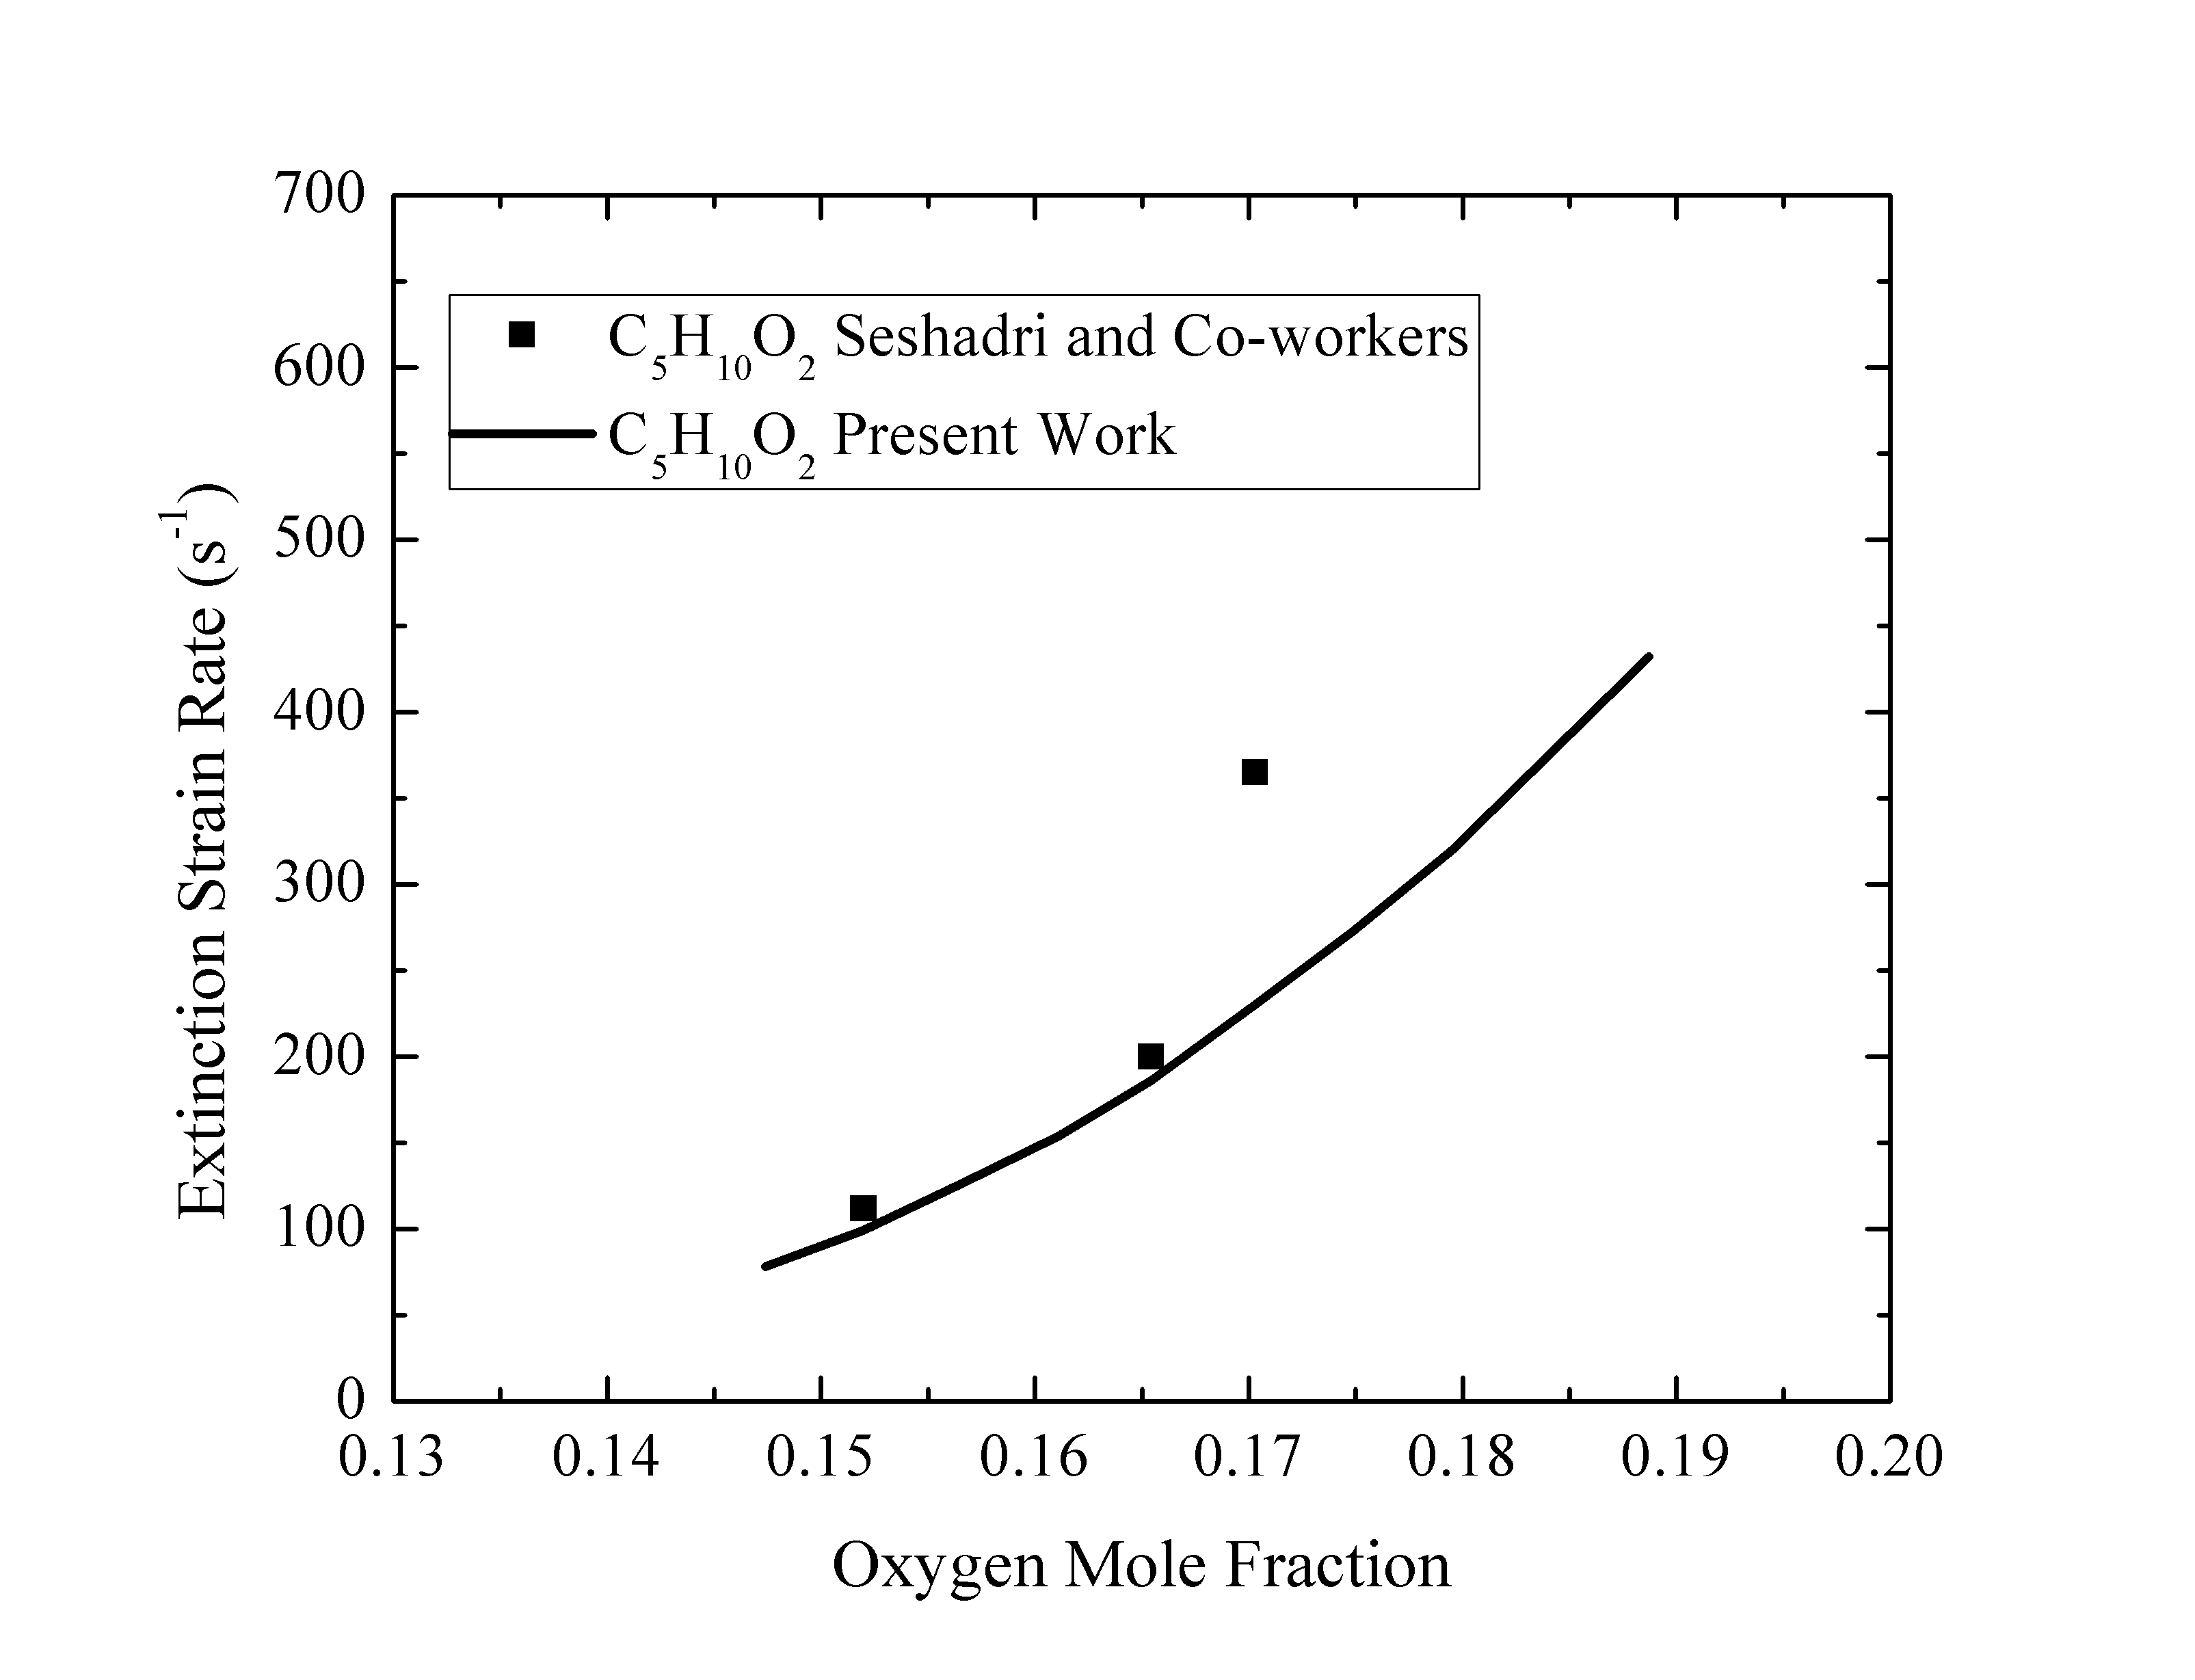
\includegraphics[trim=4mm 8mm 30mm 20mm, clip=true, width=0.4\textwidth]{MB-ESR.png}
  \normalsize
  \vspace{-0.1in}
  \caption{Mechanism validation against the extinction strain rates measurements in nonpremixed stagnation-flow systems.}
  \label{fig:validation-ESR}
\end{figure}

\subsection{Soot Model}

The detailed soot model is based on the Hybrid Method of Moments (HMOM) developed by Mueller \emph{et al.}~\cite{mueller09a,mueller09b,mueller11a}. The detailed model describes particles with both their volume and surface area and considers particle nucleation from PAH dimers~\cite{schuetz02,wong09,blanquart09c}, PAH condensation~\cite{park03,mitchell98,mitchell03}, particle coagulation~\cite{mueller09b}, surface growth by the HACA mechanism~\cite{frenklach91}, oxidation~\cite{kazakov95,neoh81}, and oxidation-induced fragmentation~\cite{mueller11a}. In addition, the model considers thermophoresis~\cite{waldmann66} but neglects molecular diffusion~\cite{bisetti12}. In total, four quantities are used to describe the evolution of the soot population: the total soot number density, the total soot volume, the total soot surface area, and the number density of smaller particles.  Further details about HMOM and the soot model can be found in Mueller \emph{et al.}~\cite{mueller09a,mueller09b,mueller11a} and the references therein.

\section{Results: Sooting Limits}
\label{sec:4}

As mentioned in Sec.~\ref{sec:2}, argon dilution was used to keep the thermal environment of the three fuel cases nearly the same.  This is justified with the simulation results of the temperature profiles for three fuel cases under the same strain rate and oxygen mole fraction, as shown in Fig.~\ref{fig:thermal}.  The difference among the peak temperatures is less than $20$ K, and the peak locations differ by less than $0.1$ mm.  Furthermore, on the fuel-rich side, in the vicinity where soot is formed, the maximum temperature difference among the fuels is less than $\pm20$ K.  Also, simulation results show that the liquid surface temperatures for all three fuels stay about $20$ K below their respective boiling points, and the liquid surface temperatures are nearly constant (within $0.3\%$), regardless of the change in oxygen mole fractions.  Consequently, the thermal environment is maintained nearly the same for all three fuels, and chemical effects have therefore been isolated from thermal effects. 


The critical strain rates (CSRs) corresponding to the sooting limits from the experiments and computations are shown in Fig.~\ref{fig:Exp-Comp}. For each set of data, the region above/left of the data corresponds to non-sooting flames, and the region below/right of the data corresponds to sooting flames. For all three fuels, the CSR increases with increasing oxygen concentration in the oxidizer stream, which has been previously characterized as a thermal effect~\cite{du91}. In addition, both experiment and computation show that methyl butanoate has substantially lower CSRs compared to  $n$-heptane and $n$-butanol. 

This distinct trend warrants further investigation.  Noting that, in this work, the CSRs are defined (experimentally and computationally) based on an absolute amount of soot, the fact that the CSRs are substantially lower for methyl butanoate compared to the other two fuels could then be due to either or both of the following hypotheses.  First, less soot is formed from methyl butanoate overall, regardless of strain rate.  Second, the chemical pathways leading to PAH and soot formation for methyl butanoate are slower and are more strongly suppressed with decreasing residence time (increasing strain rate).  The relative roles of these two hypotheses require further analysis.

\begin{figure}[t]
  \centering
  \scriptsize
  \vspace{-0.1in}
  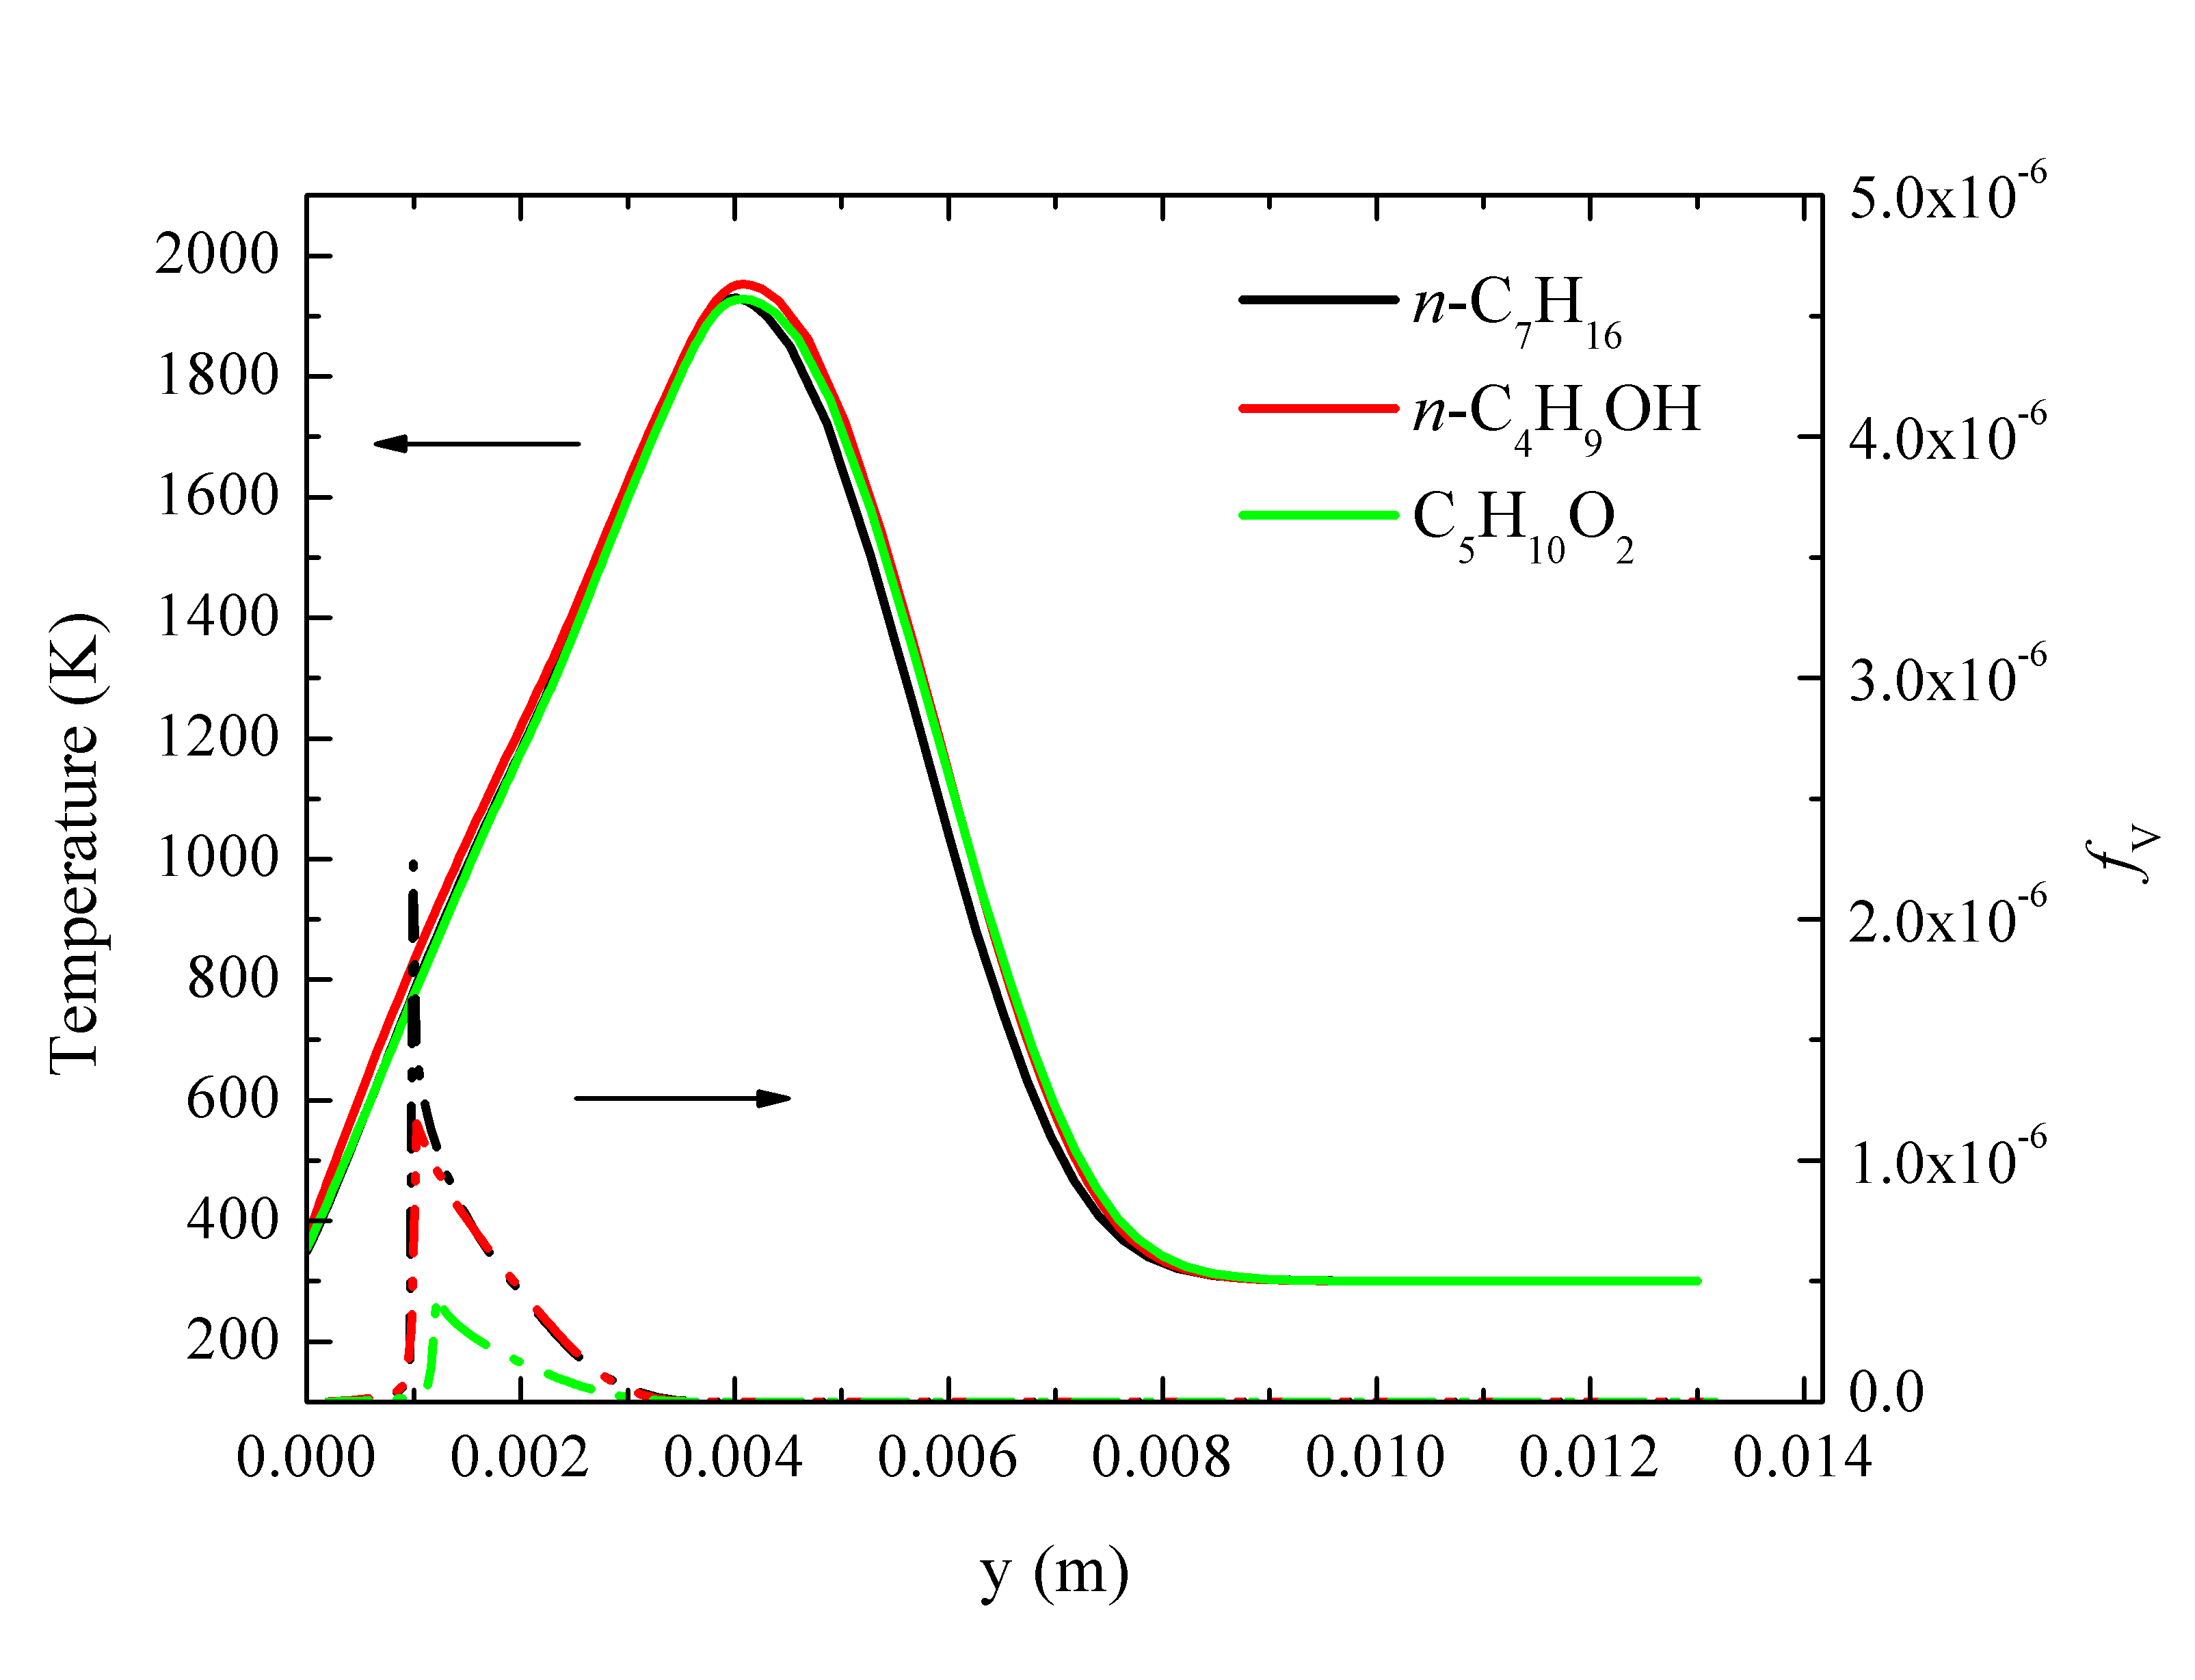
\includegraphics[trim=4mm 8mm 4mm 20mm, clip=true, width=0.5\textwidth]{Thermal.png}
  \normalsize
  \vspace{-0.1in}
  \caption{Temperature (solid line) and $f_V$ (dash-dotted line) profiles at the strain rate of $16$ s$^{-1}$ and $X_{O_2}=0.2$.}
  \label{fig:thermal}
\end{figure}


\begin{figure}[t]
  \centering
  \scriptsize
  \vspace{0.5in}
  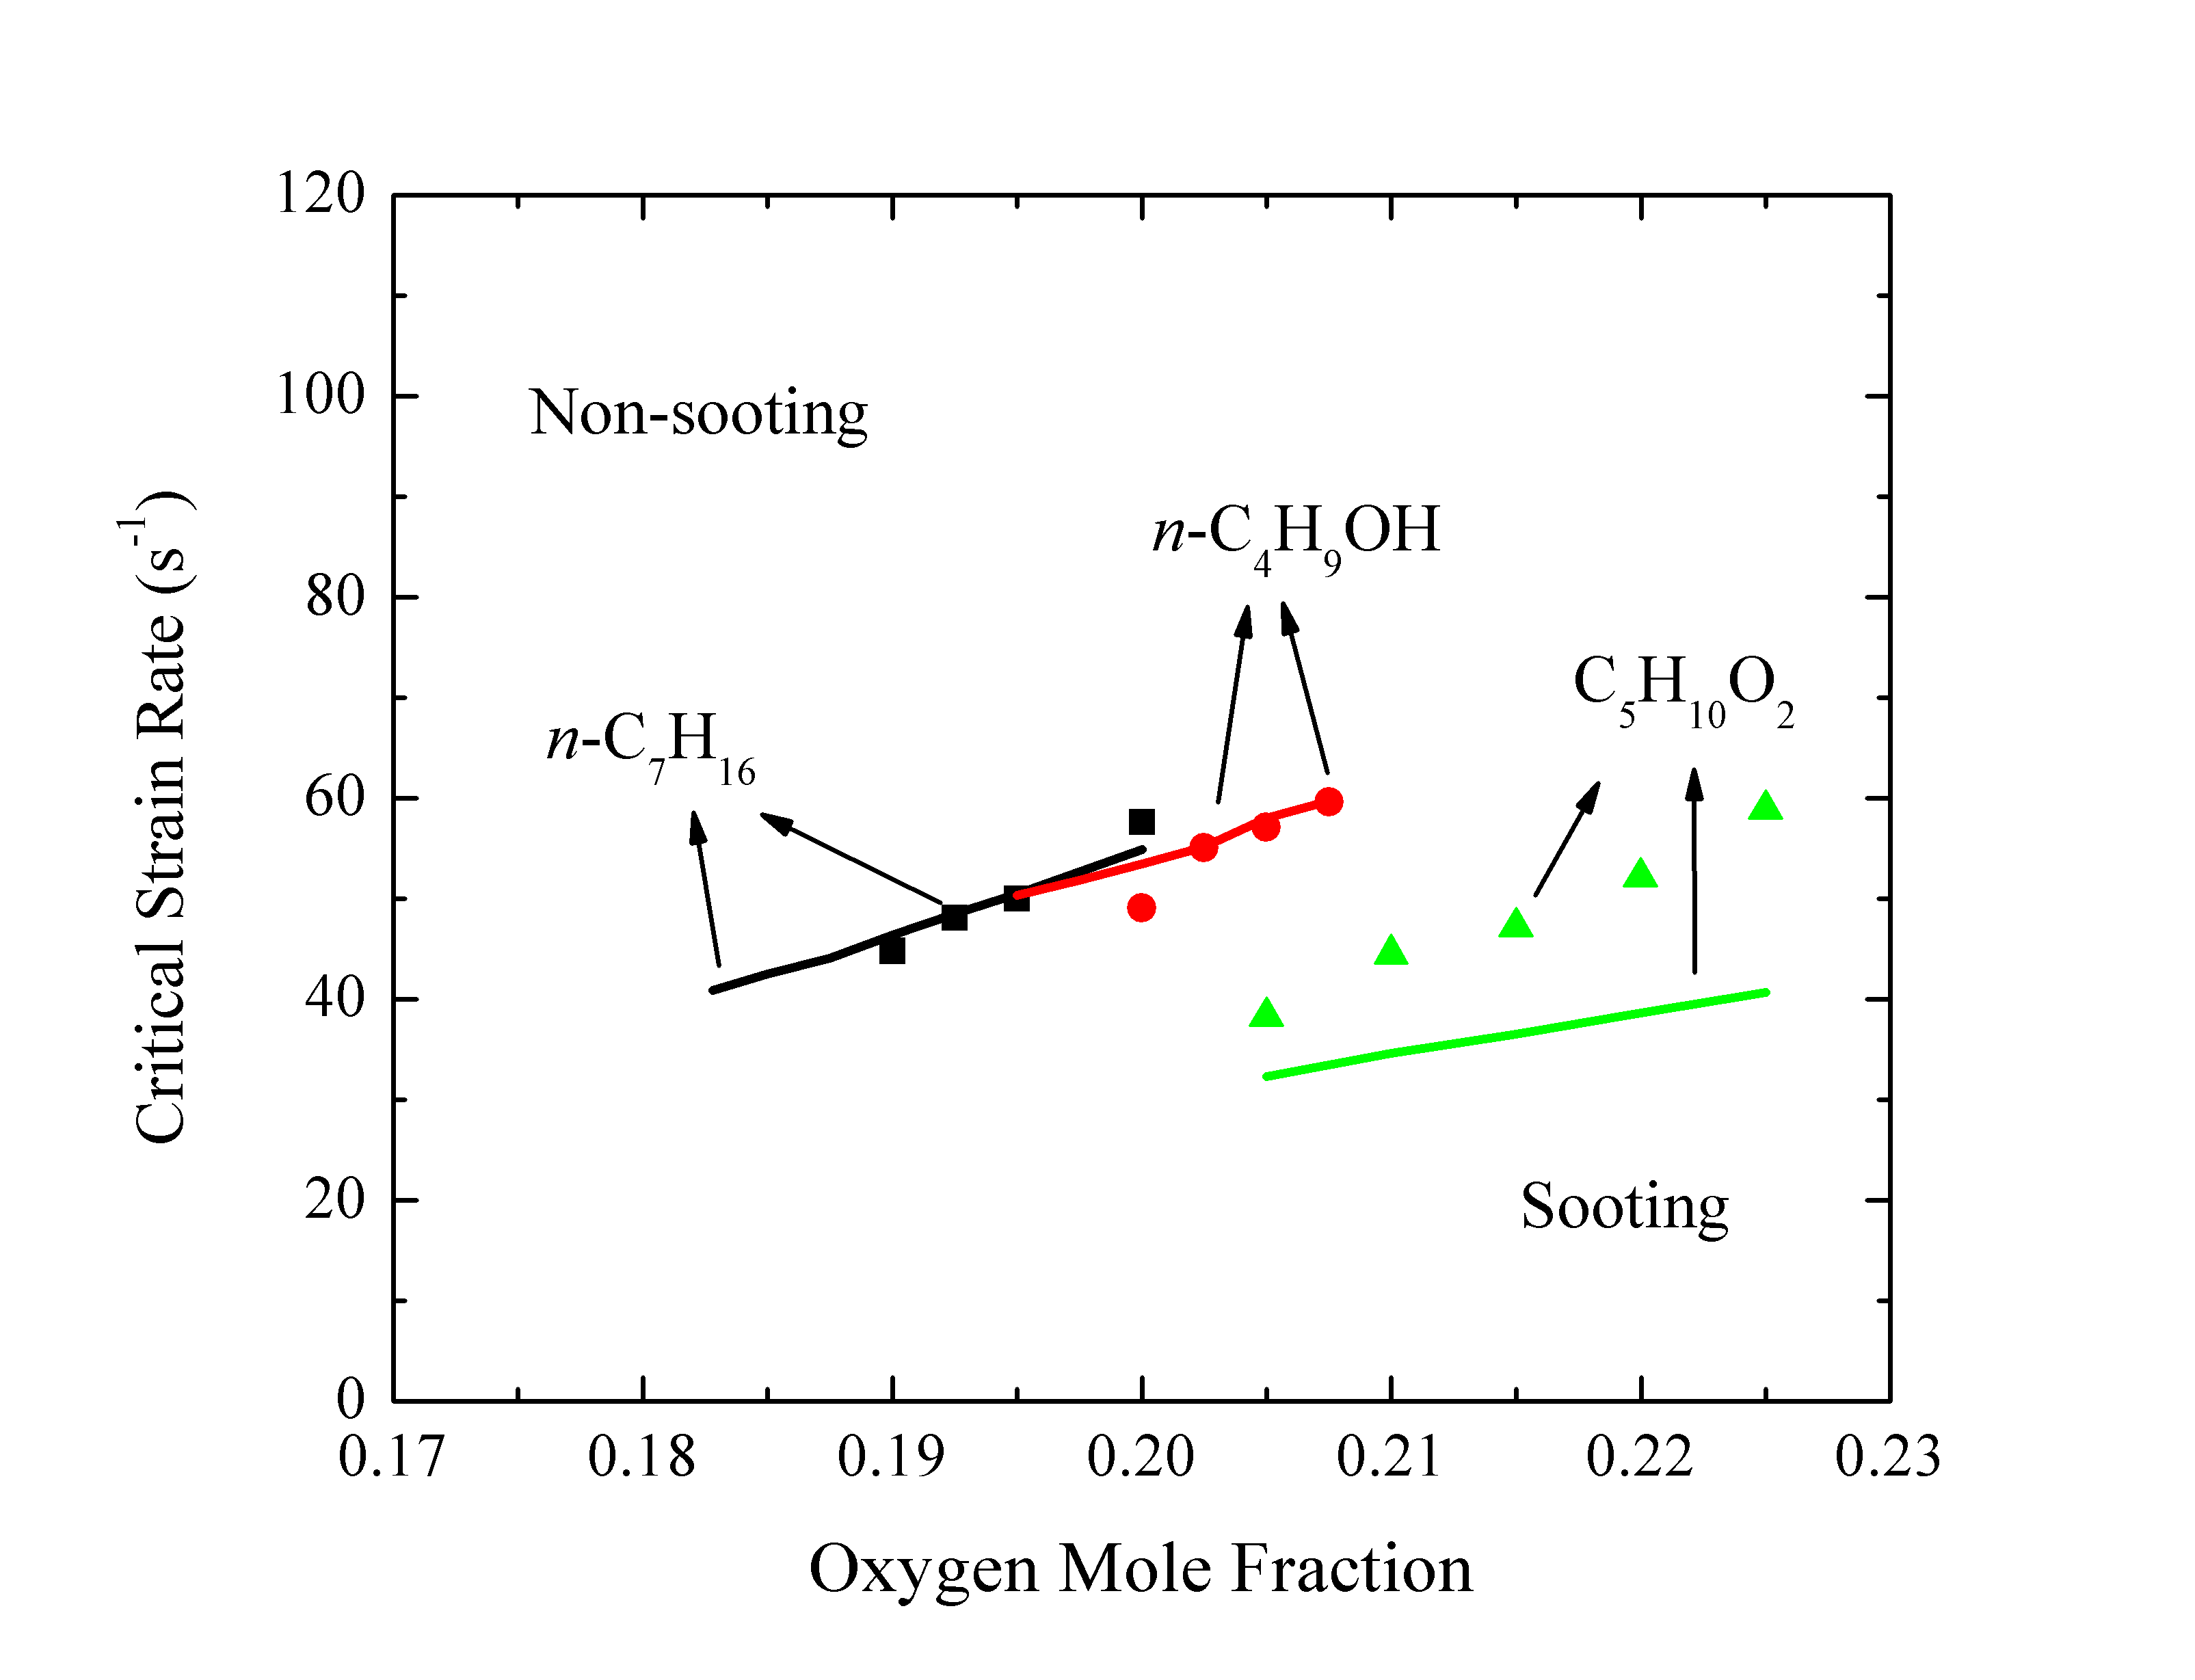
\includegraphics[trim=4mm 8mm 30mm 20mm, clip=true, width=0.5\textwidth]{Exp-Comp.png}
%  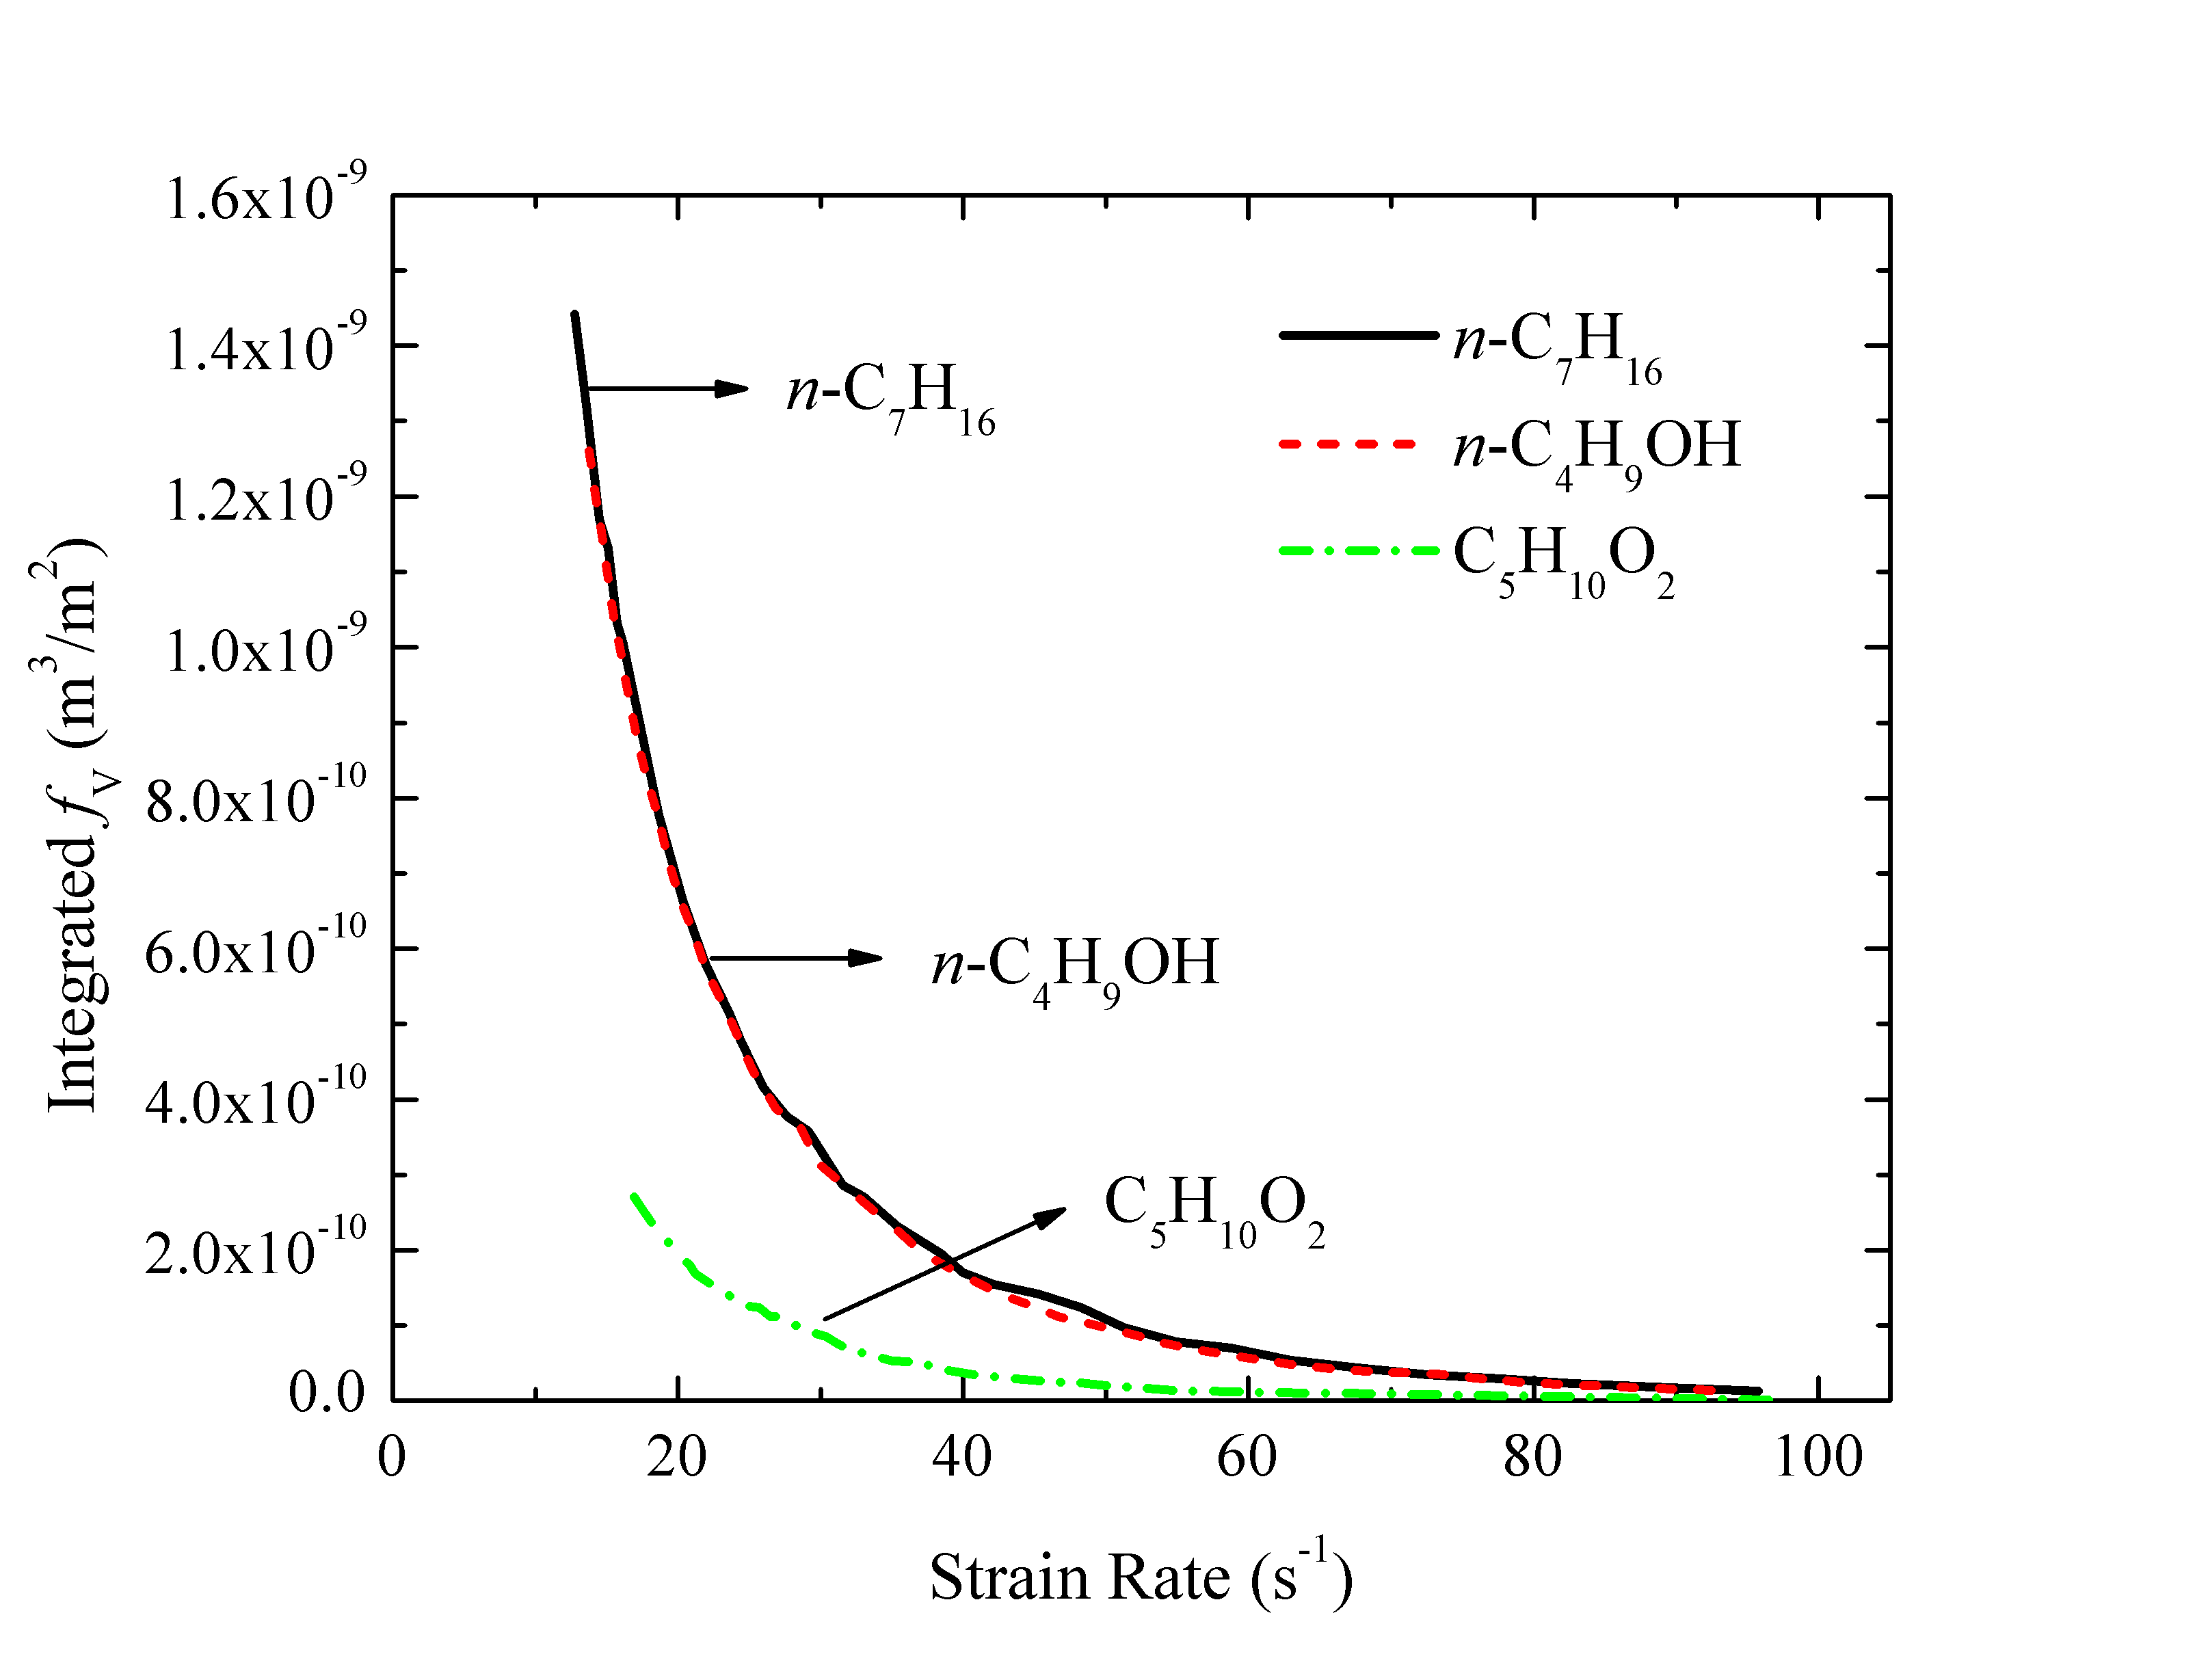
\includegraphics[trim=4mm 8mm 30mm 20mm, clip=true, width=0.48\textwidth]{SV-SR.png}
  \normalsize
  \vspace{-0.1in}
  \caption{Experimental (symbols) and computational (lines) CSRs.}
  \label{fig:Exp-Comp}
\end{figure}

\begin{figure}[t]
  \centering
  \scriptsize
  \vspace{-0.1in}
%  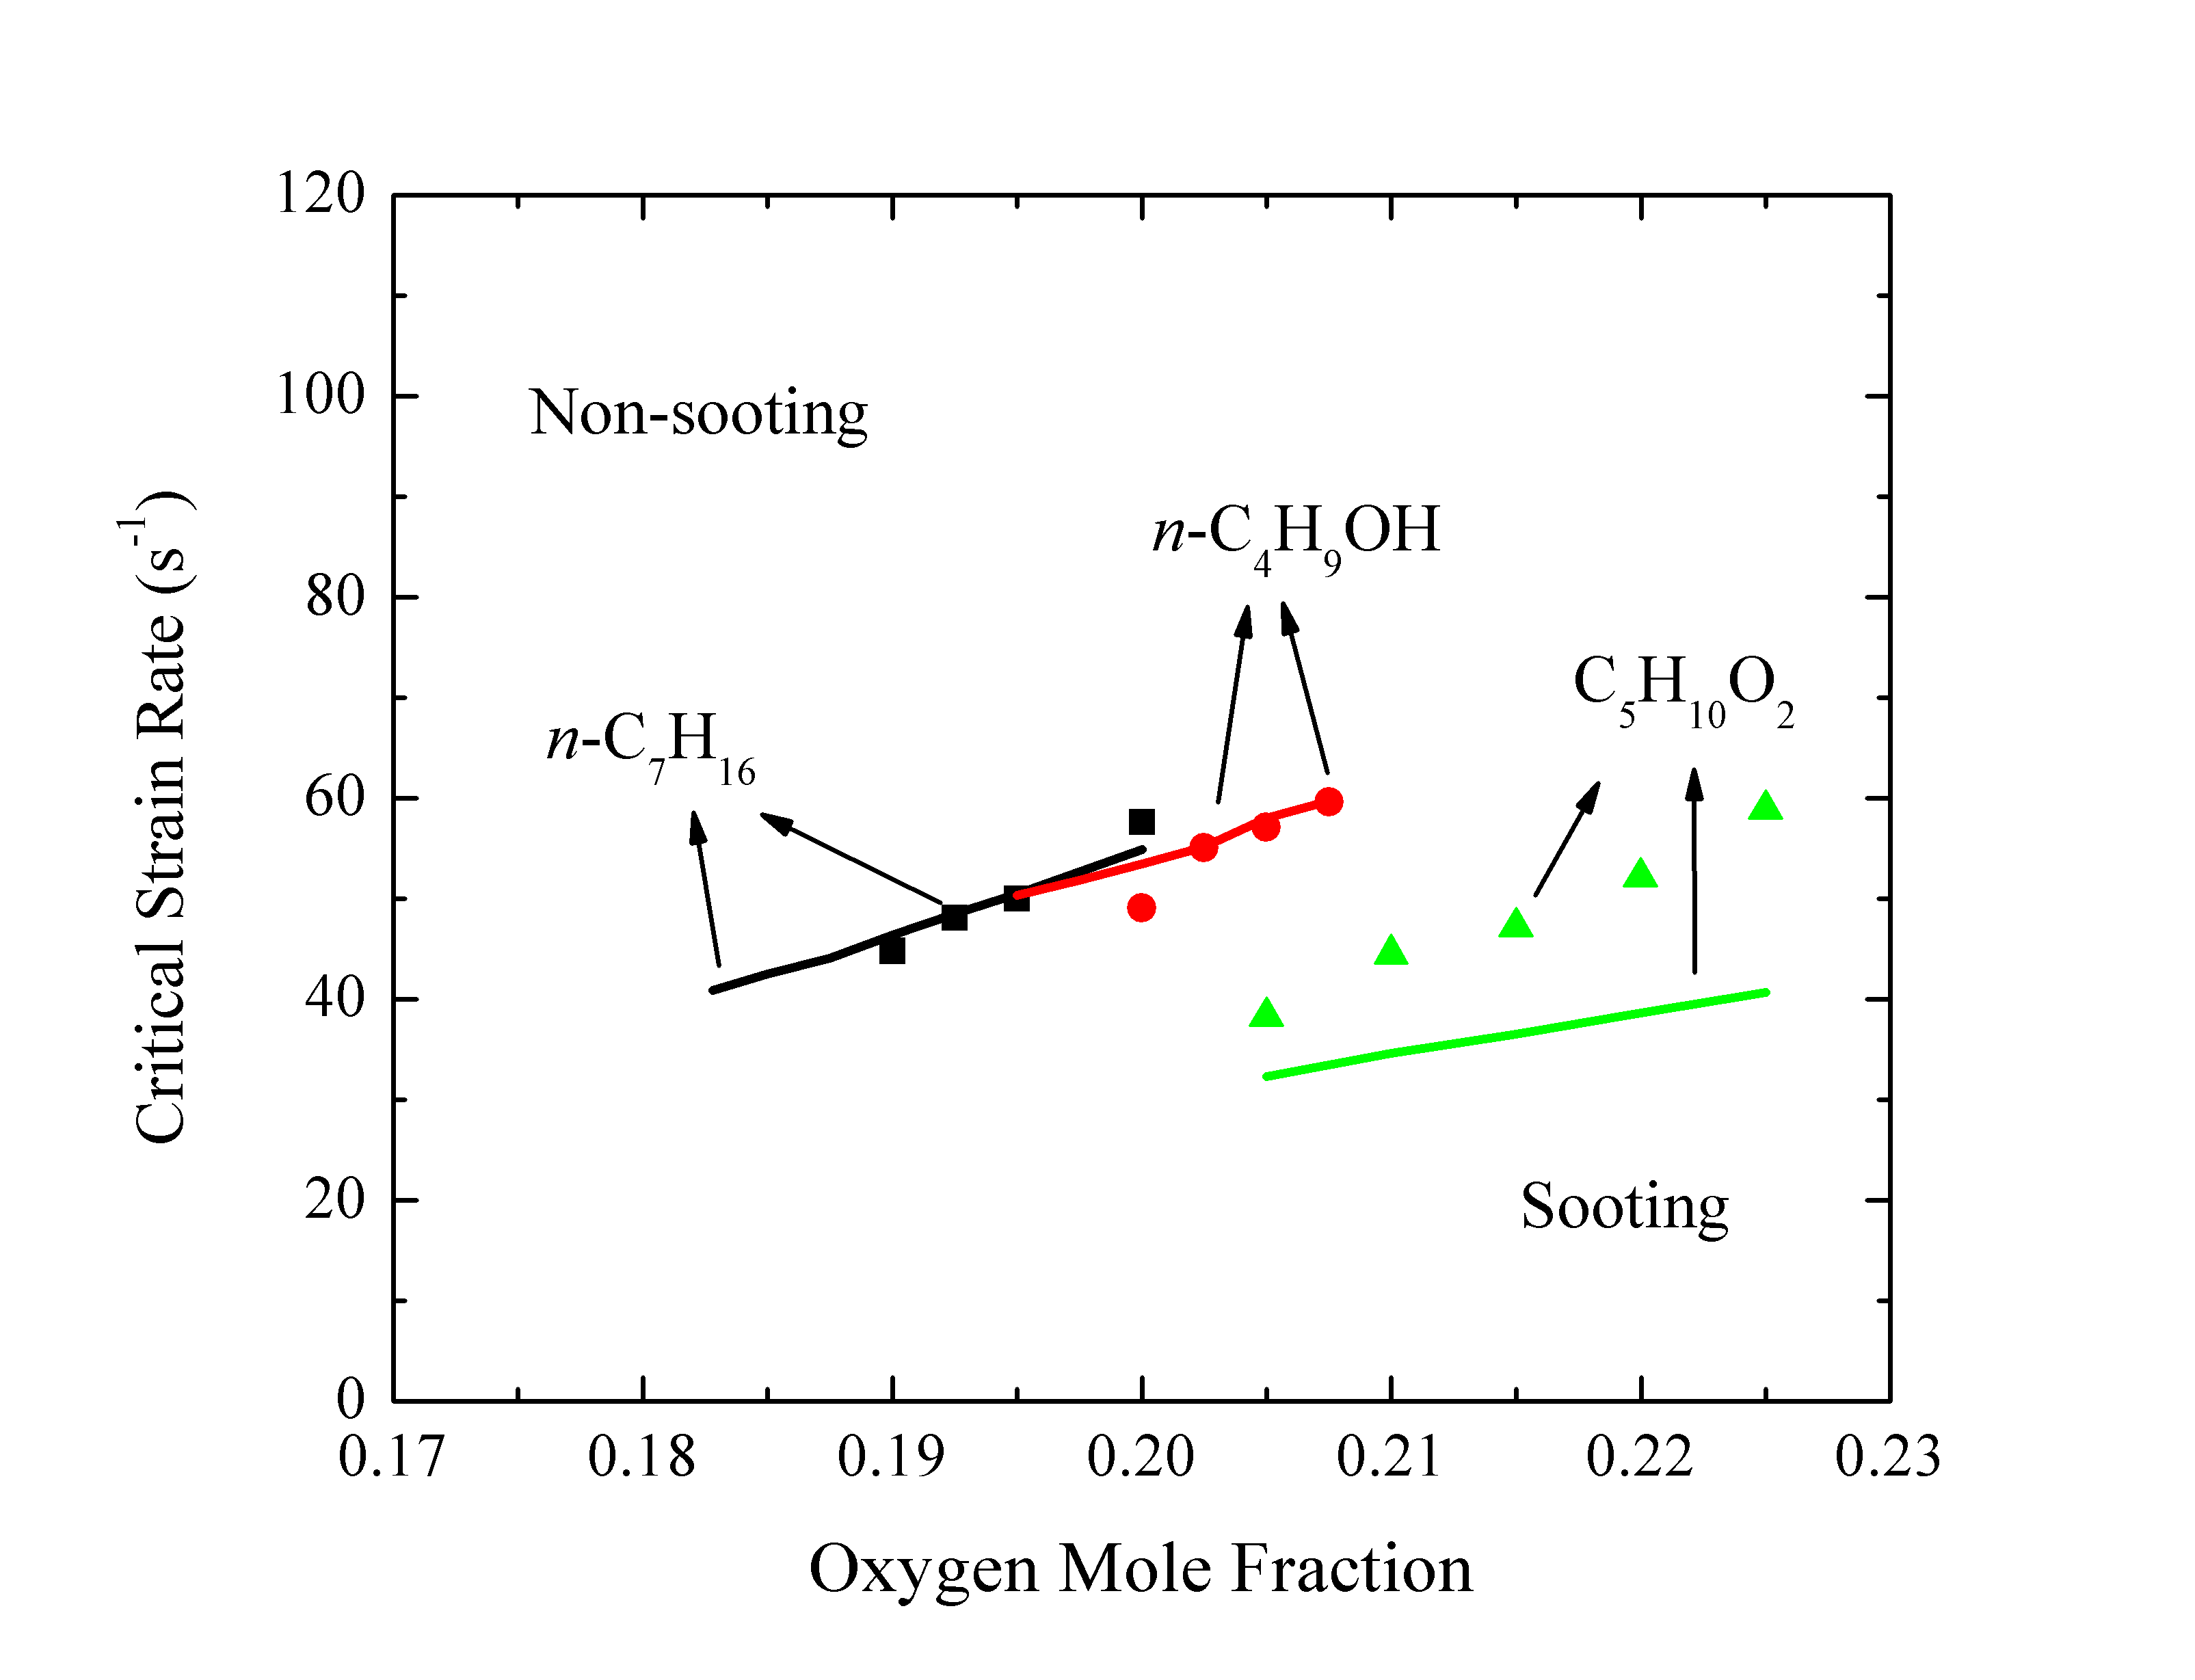
\includegraphics[trim=4mm 8mm 30mm 20mm, clip=true, width=0.48\textwidth]{Exp-Comp.png}
  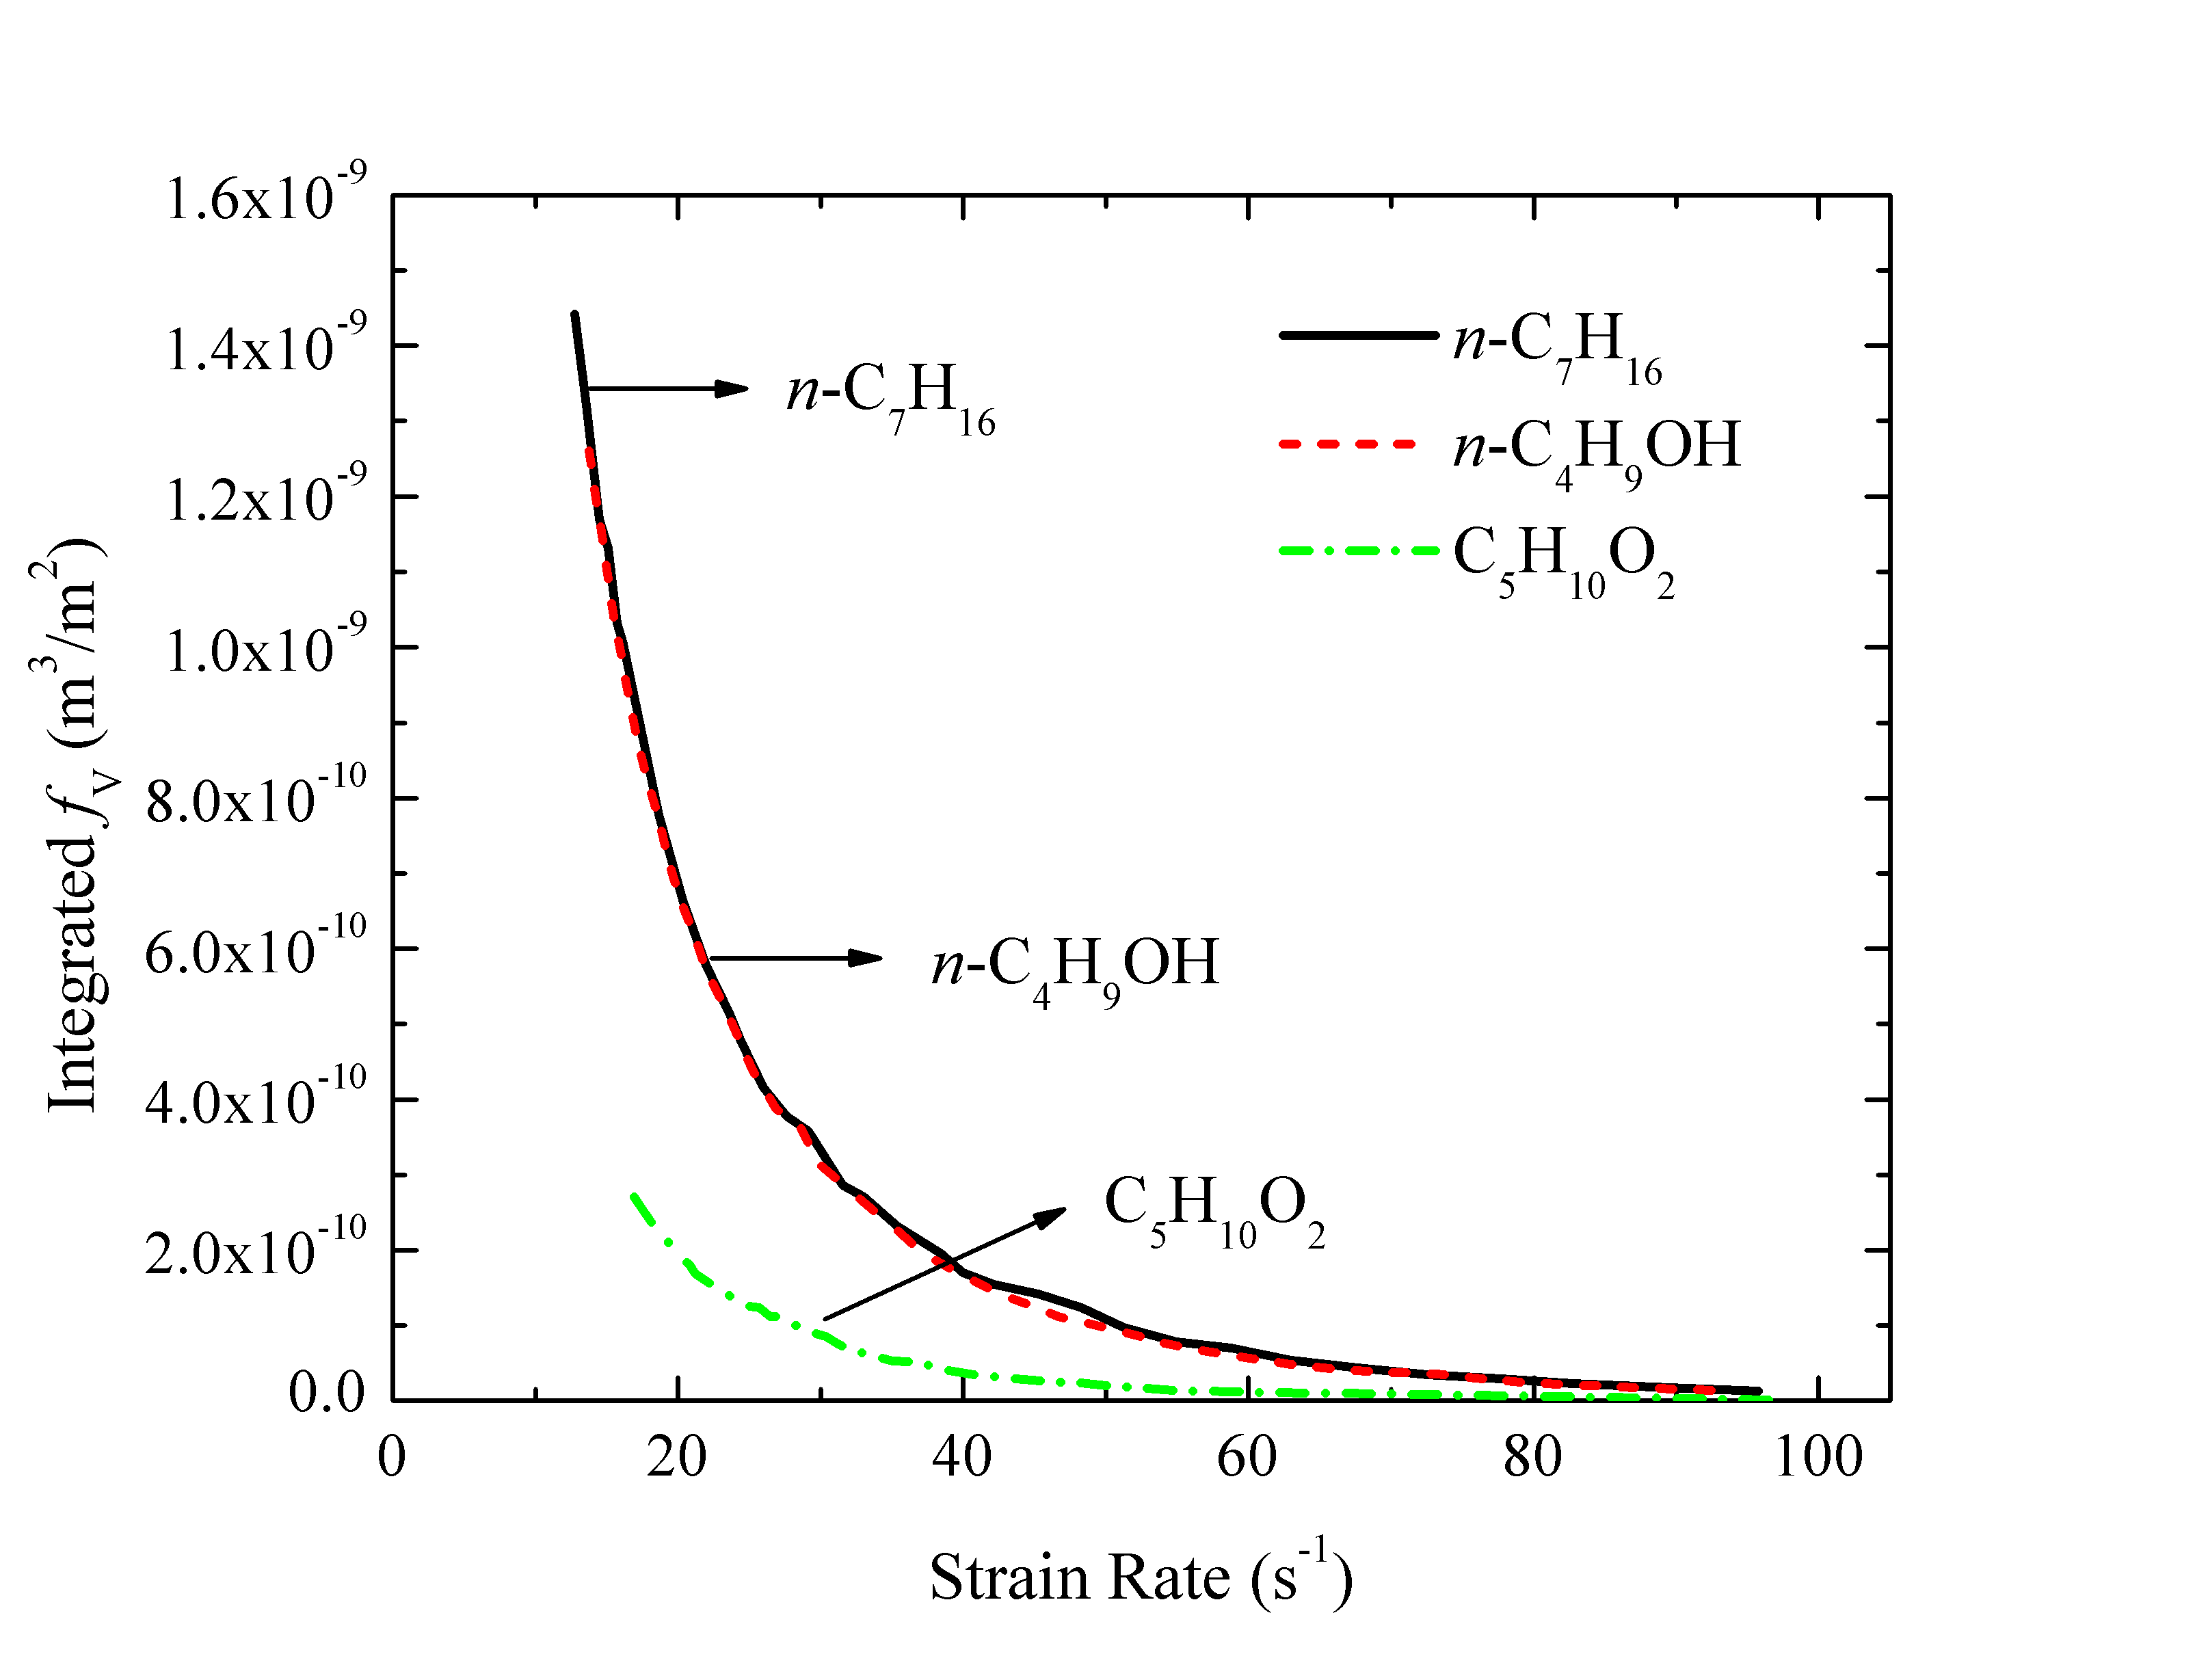
\includegraphics[trim=4mm 8mm 30mm 20mm, clip=true, width=0.5\textwidth]{SV-SR.png}
  \normalsize
  \vspace{-0.1in}
  \caption{The responses of the integrated $f_V$ to strain rate at $X_{O_2}=0.2$.}
  \label{fig:fv}
\end{figure}


\section{Mechanistic Analysis}

To elucidate the role of the above two hypotheses, mechanistic analysis was conducted for all three fuels to investigate the response of soot volume fraction to strain rate, chemical pathways for PAH formation, and the rate-limiting steps for PAH formation for each of the three fuels.

\subsection{Volume Fraction Response to Strain Rate}

The integrated $f_V$ under various strain rates are shown in Fig.~\ref{fig:fv}.  For all three fuels, as the strain rate increases, less soot is formed due to reduced residence time.  At all strain rates, $n$-butanol is overall as sooty as $n$-heptane, while methyl butanoate is the least sooty.  If a critical $f_V$ is chosen and a horizontal line drawn based on this choice, the intersections of the horizontal line and the three $f_V$ profiles give the corresponding CSRs for the three fuels.  This is indeed how the computational CSRs were determined in the current study.  Therefore, the CSRs correlate with the total amount of soot formed, explaining at least in part the CSR trends. However, detailed chemical pathway analysis is still needed to elucidate the differences in the global sooting behavior as well as to see if there are any significant differences in PAH pathways with different timescales for the three fuels that could further explain the observed trends in CSRs.

\subsection{Sensitivity and Reaction Pathway Analysis}

To understand the distinct differences in PAH evolution between the three fuels, sensitivity and reaction path analysis were performed for a representative PAH species, naphthalene (C$_{10}$H$_8$).  As shown in Fig.~\ref{fig:SA4} and Fig.~\ref{fig:Pathways_PAH}, naphthalene shows roughly the same sensitivities to the same reactions for each of the fuels, and the chemical pathways of naphthalene are essentially the same after the fuel cracking. Initially, fuel cracks to unsaturated C$_3$ to C$_5$ chains through H abstraction followed by $\beta$-scission reactions. These smaller molecules further decompose into allyl radicals (CH$_2$=CH-CH$_2^*$ or A-C$_3$H$_5$) and propene (C$_3$H$_6$), which contribute to C$_5$ and C$_6$ ring formation by either combining with acetylene (C$_2$H$_2$) or forming propargyl (C$_3$H$_3$), the latter further combining with itself to form aromatic rings. Larger species (predominantly toluene and indene) are formed by the combination of benzene and cyclopentadiene with smaller species, such as 
CH$_3$, C$_2$H$_2$, and C$_3$H$_3$. Two pathways directly contribute to naphthalene formation, namely, cyclopentadienyl (C$_5$H$_5$) radical recombination and methyl addition to indenyl (C$_9$H$_7$)
\begin{align*}
  2 {\rm C}_5{\rm H}_5 &\longrightarrow {\rm C}_{10}{\rm H}_8 + 2 {\rm H}\\
  {\rm C}_9{\rm H}_7 + {\rm C}{\rm H}_3 &\longrightarrow {\rm C}_{10}{\rm H}_8 + 2 {\rm H}.
\end{align*}


\begin{figure}[t]
  \centering
  \scriptsize
%  \vspace{-0.4in}
%  \hspace{-0.8in}
  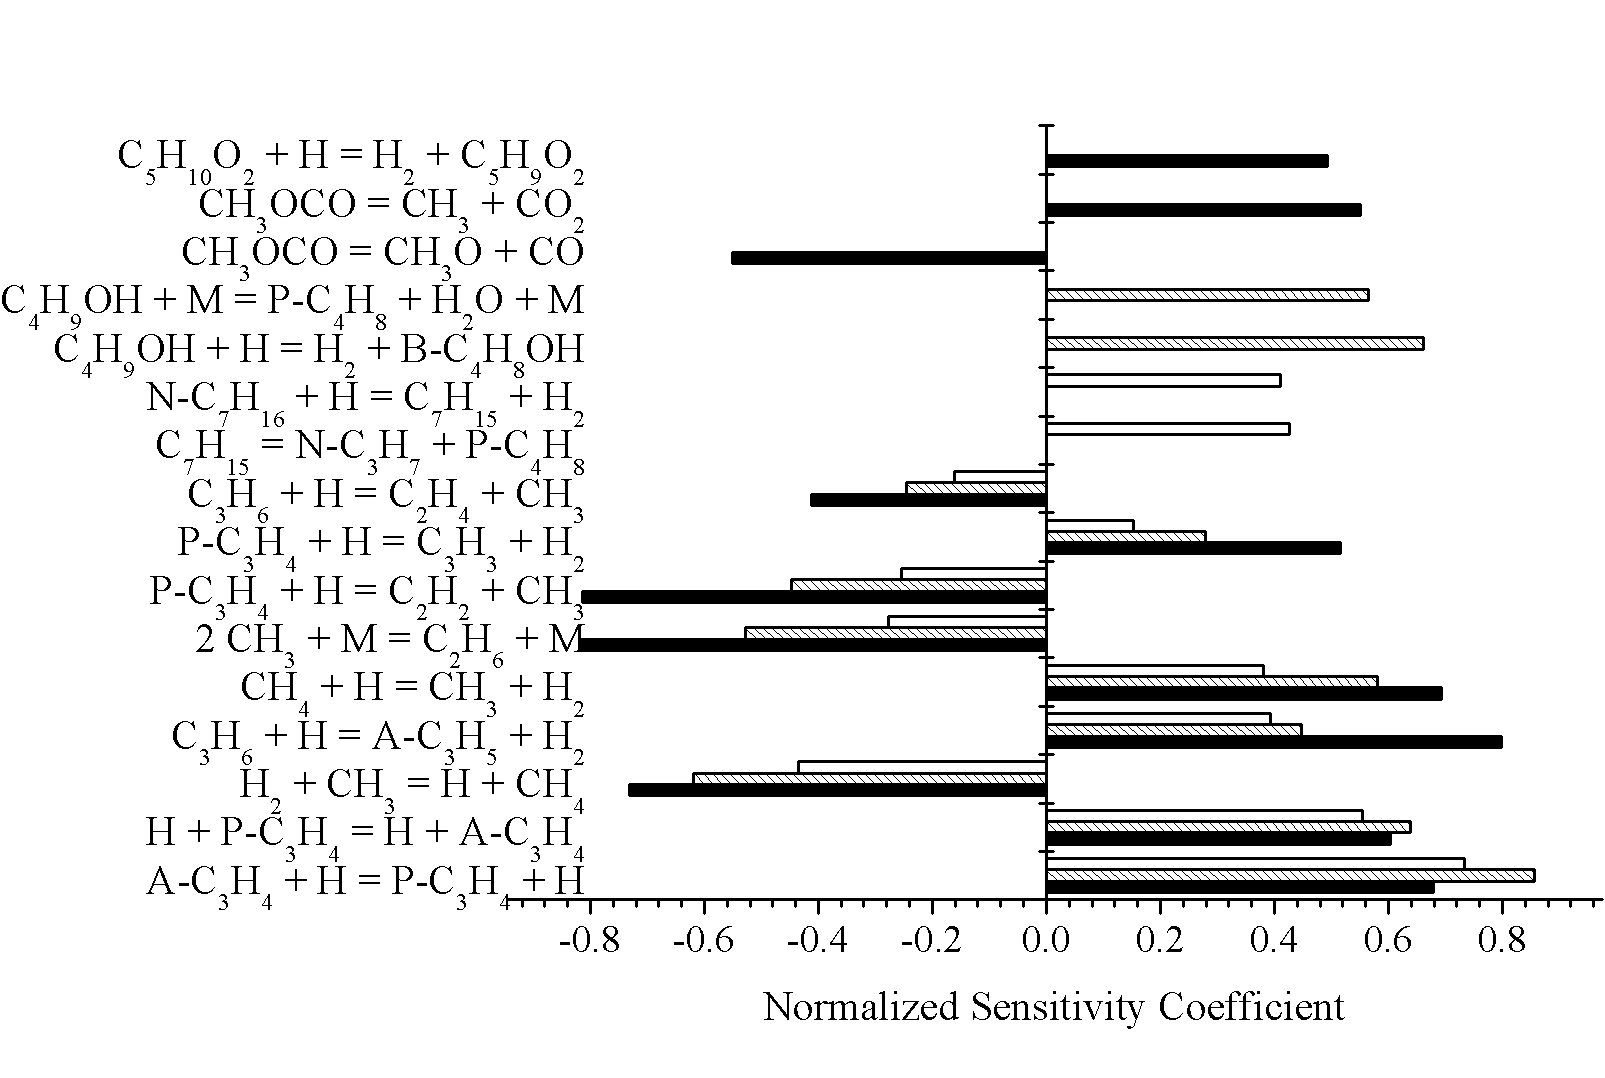
\includegraphics[trim=0mm 0mm 0mm 8mm, clip=true,width=0.49\textwidth]{Chain.png}
  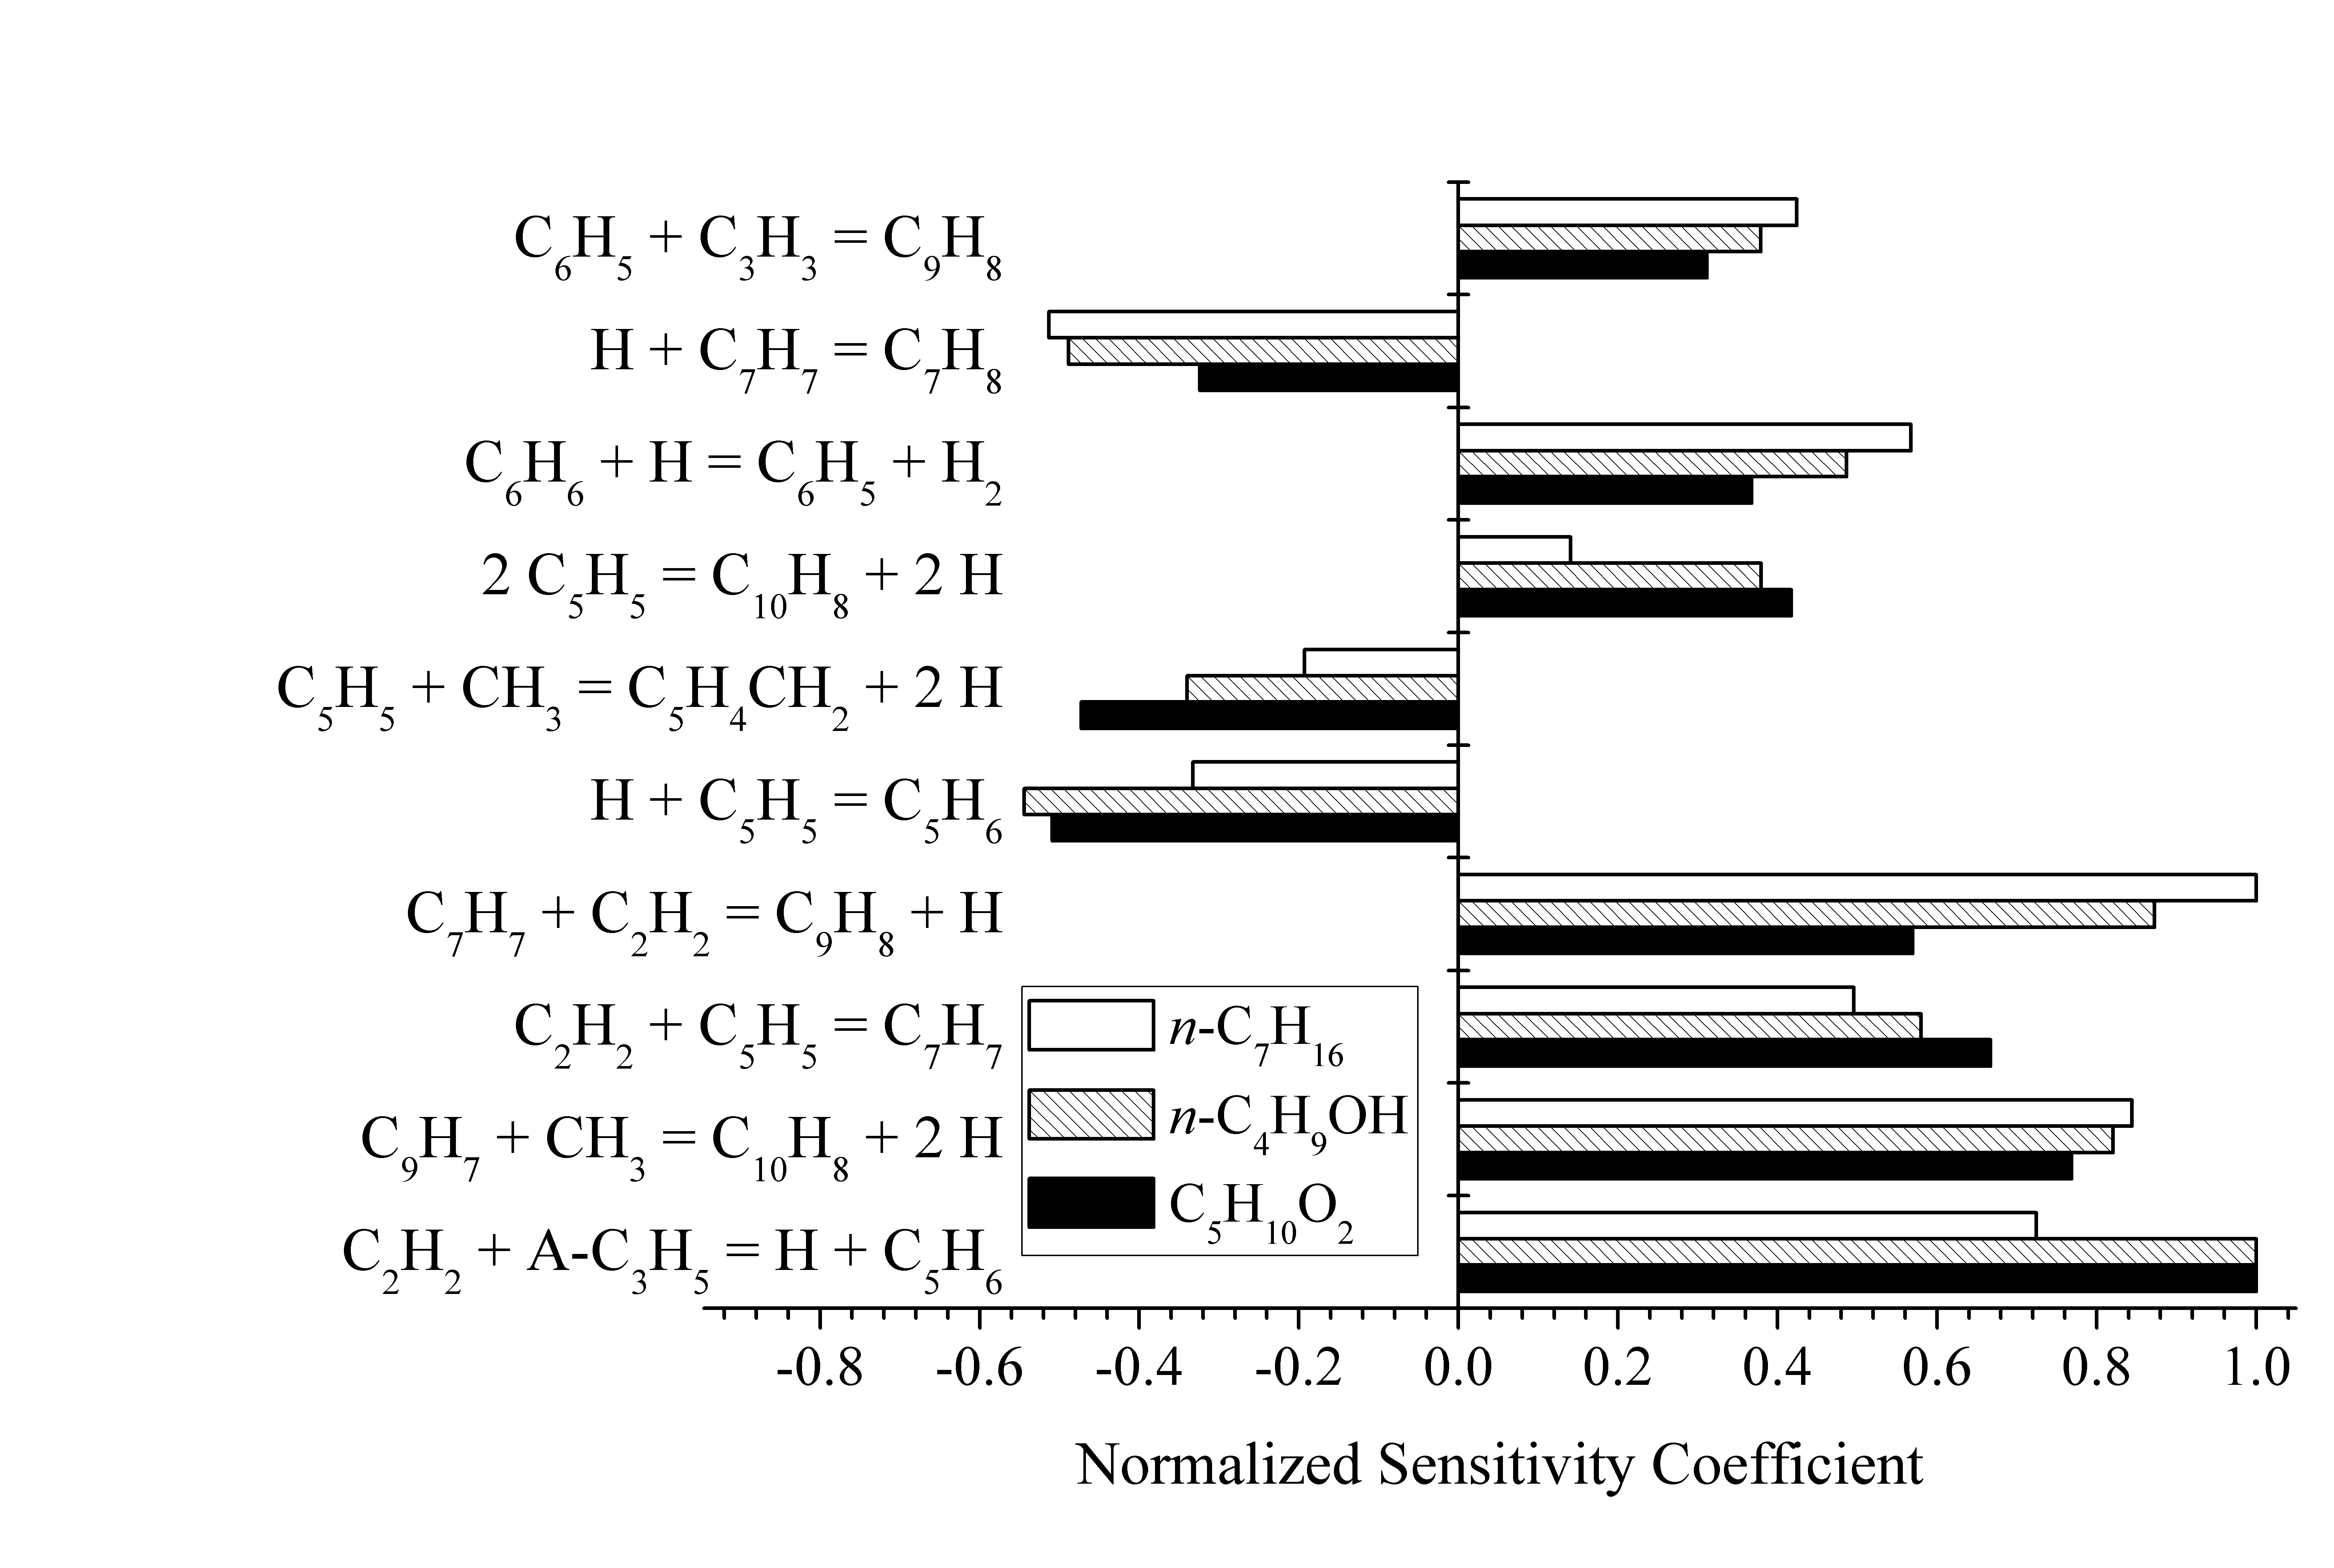
\includegraphics[trim=0mm 0mm 0mm 8mm, clip=true,width=0.49\textwidth]{Ring.png}
  \normalsize
  \vspace{-0.2in}
  \caption{Sensitivity of the maximum naphthalene mass fraction to kinetics at the strain rate of $16$ s$^{-1}$ and $X_{O_2}=0.2$. Left: Intermediate chain radical reactions. Right: Ring formation reactions.}
  \label{fig:SA4}
\end{figure}

Although the PAH pathways for the three fuels are similar, the formation of these soot precursors from the fuel cracking processes and the relative importance of the subsequent chemical pathways of PAH growth are fuel specific. Noting the similarity in the chemical pathways beyond A-C$_3$H$_5$ and C$_3$H$_6$, the fuel specific breakdown pathways that lead to the generation of these precursors are depicted in Fig.~\ref{fig:Pathways_Fuel}. For both $n$-heptane and $n$-butanol, 1-butene (P-C$_4$H$_8$) is a product of the fuel decomposition, and this species contributes to $25\%$ of A-C$_3$H$_5$ production and strongly promotes naphthalene formation, as indicated by the sensitivity analysis in Fig.~\ref{fig:SA4}. Moreover, the fuel bound oxygen in $n$-butanol is converted into water during an intramolecular water elimination reaction and does not contribute to carbon reduction~\cite{mcenally05,mcenally11}.  As a consequence, P-C$_4$H$_8$ is also formed from the water elimination reaction, which explains the similar sooting behavior as $n$-heptane.

Conversely, C$_3$ species are the largest species formed from methyl butanoate cracking due to the fuel bound oxygen. As pointed out by Westbrook \emph{et al.}~\cite{westbrook06}, the double C=O bond is very difficult to break, so the carbon chain length is reduced when the C-C bond is broken due to $\beta$-scission. The oxygenated parts are then oxidized to CO and CO$_2$, preventing the carbon from entering the pool for soot formation~\cite{feng12,wangyl11}. As shown in Fig.~\ref{fig:CxHy}, fewer allyl radicals are formed from methyl butanoate, such that the concentration of C$_5$H$_5$ is also reduced. Since one of the pathways for naphthalene depends quadratically on C$_5$H$_5$, even moderate reductions in the radical concentration will significantly reduce naphthalene. As a result, in methyl butanoate flames, the C$_5$H$_5$ recombination pathway is negligible compared to the C$_9$H$_7$ pathway. This reduction in soot precursors from fuel cracking processes distinguishes methyl butanoate from $n$-heptane 
and $n$-butanol, in terms of the sooting propensity and CSR.

\begin{figure*}[t]
  \centering
  \scriptsize
%  \vspace{-0.4in}
%  \hspace{-0.4in}
  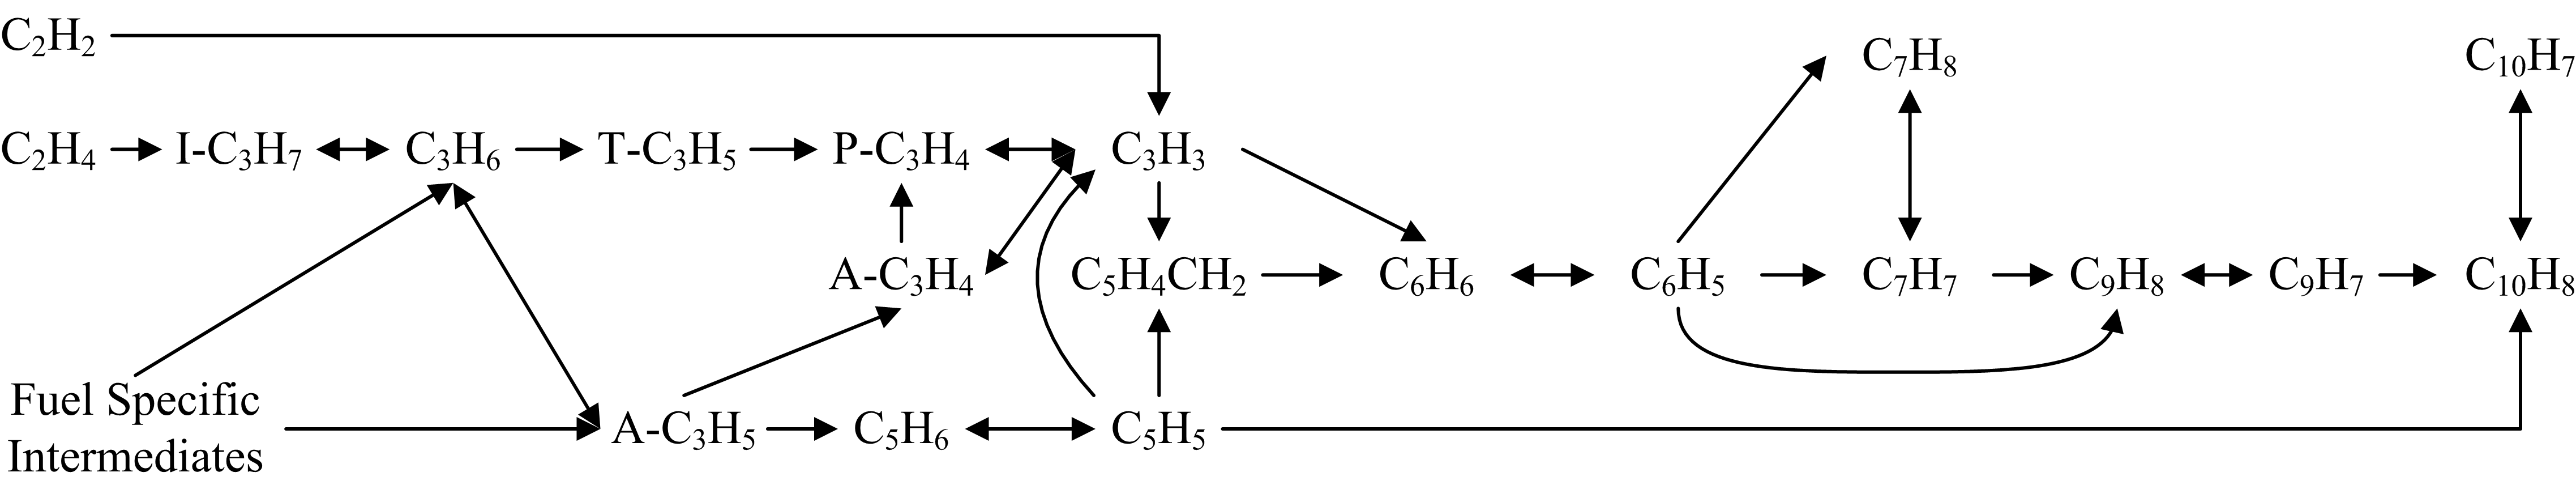
\includegraphics[width=0.8\textwidth]{Pathways-PAH.png}
  \normalsize
  \caption{Chemical pathways for naphthalene formation at the strain rate of $16$ s$^{-1}$ and $X_{O_2}=0.2$.}
  \label{fig:Pathways_PAH}
\end{figure*}

\begin{figure*}[t]
  \centering
  \scriptsize
%  \vspace{-0.4in}
%  \hspace{-0.4in}
  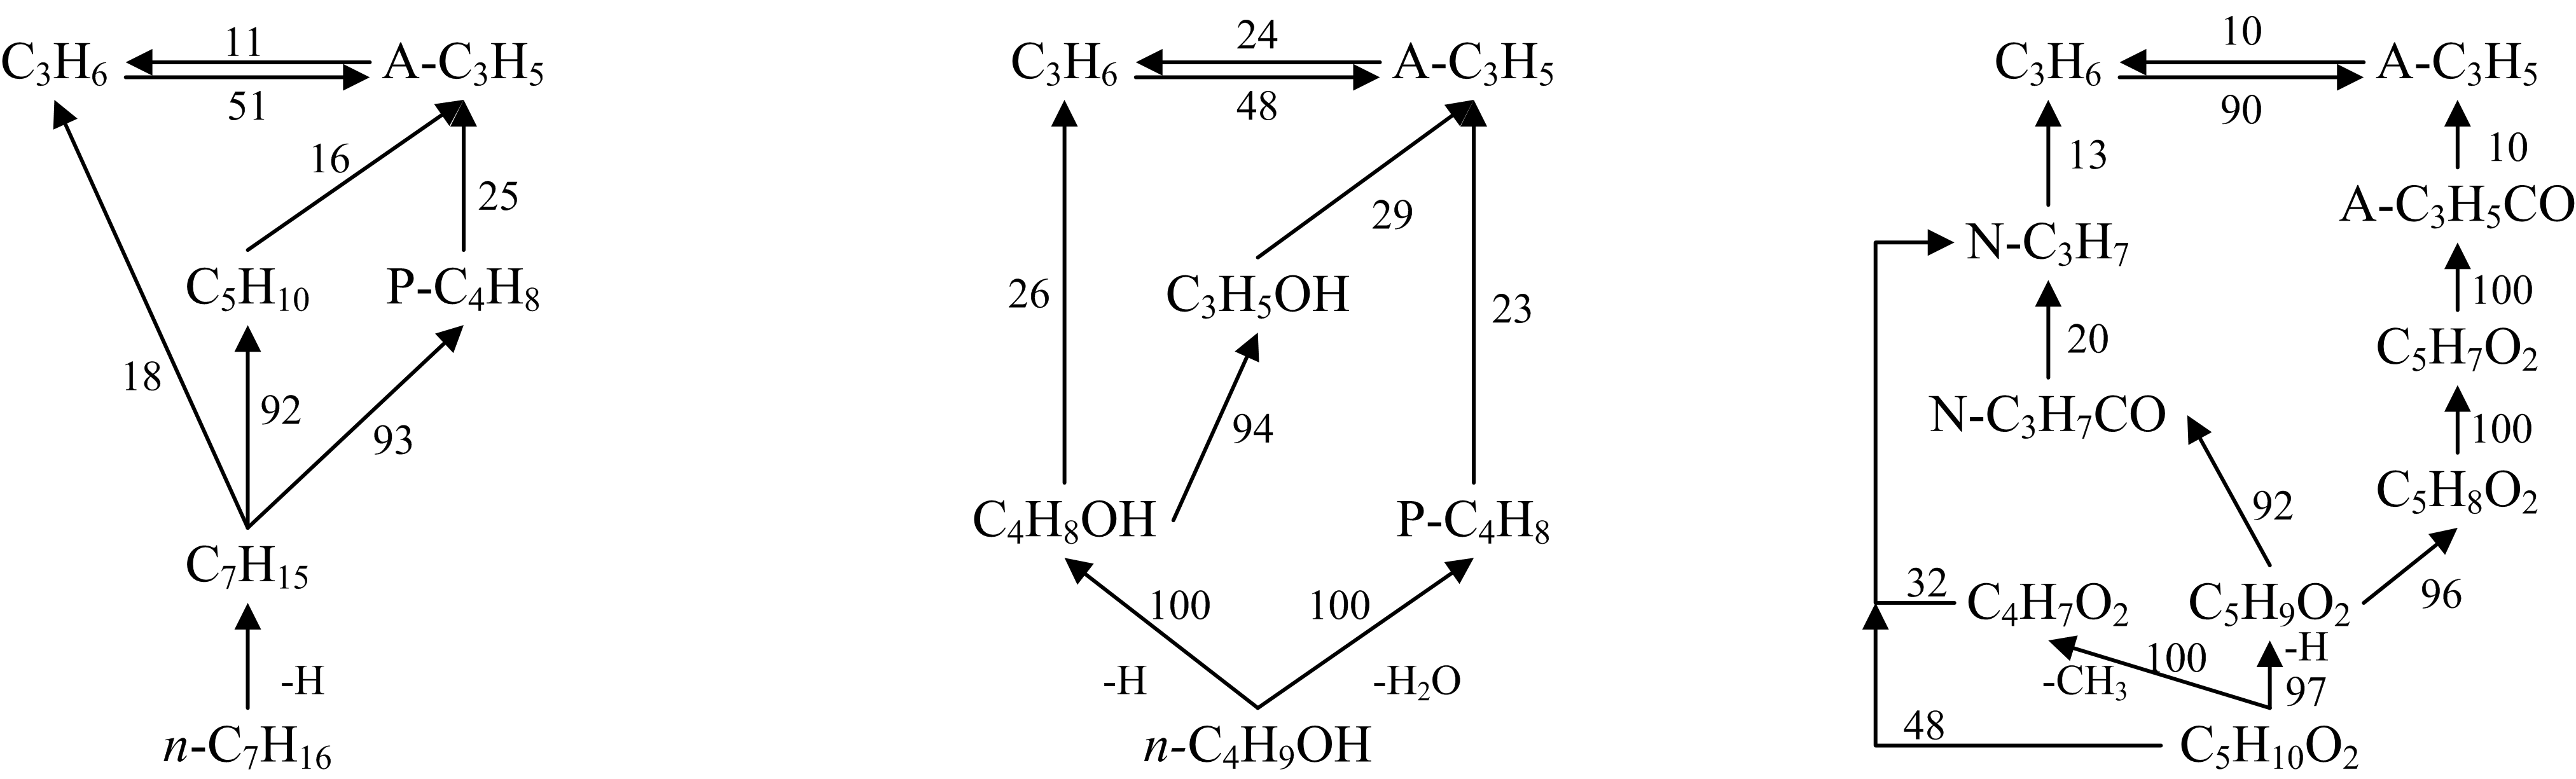
\includegraphics[width=0.8\textwidth]{Pathways_Fuel.png}
  \normalsize
  \caption{Fuel specific pathways for C$_3$H$_6$ and A-C$_3$H$_5$ formation at the strain rate of $16$ s$^{-1}$ and $X_{O_2}=0.2$. From left to right: $n$-heptane, $n$-butanol, and methyl butanoate.  The numbers indicate the relative contribution (in percentages) to the formation of the ``downstream'' species.}
  \label{fig:Pathways_Fuel}
\end{figure*}

At this point, the pathways and species that are responsible for soot formation have been identified. The next question that naturally arises is how sensitive these pathways are to the increasing strain rate that leads to reduced soot formation. Although not shown here, sensitivity and reaction path analysis was conducted at critical strain rates, and no substantial differences were found compared with low strain rate cases. In addition, if the CSR is defined based on a relative metric, in other words, to be the strain rate at which the global domain-integrated $f_V$ is $10\%$ of the value at a fixed low strain rate ($16$ s$^{-1}$), the three fuels have essentially the same CSR, indicating the potential similarity in the rate-limiting steps of soot formation. These observations indicate that it is mostly the total amount of soot formed with the three fuels that give the differences in CSR.

%\begin{figure*}[h]
%  \centering
%  \scriptsize
%%  \vspace{-0.4in}
%%  \hspace{-0.4in}
%  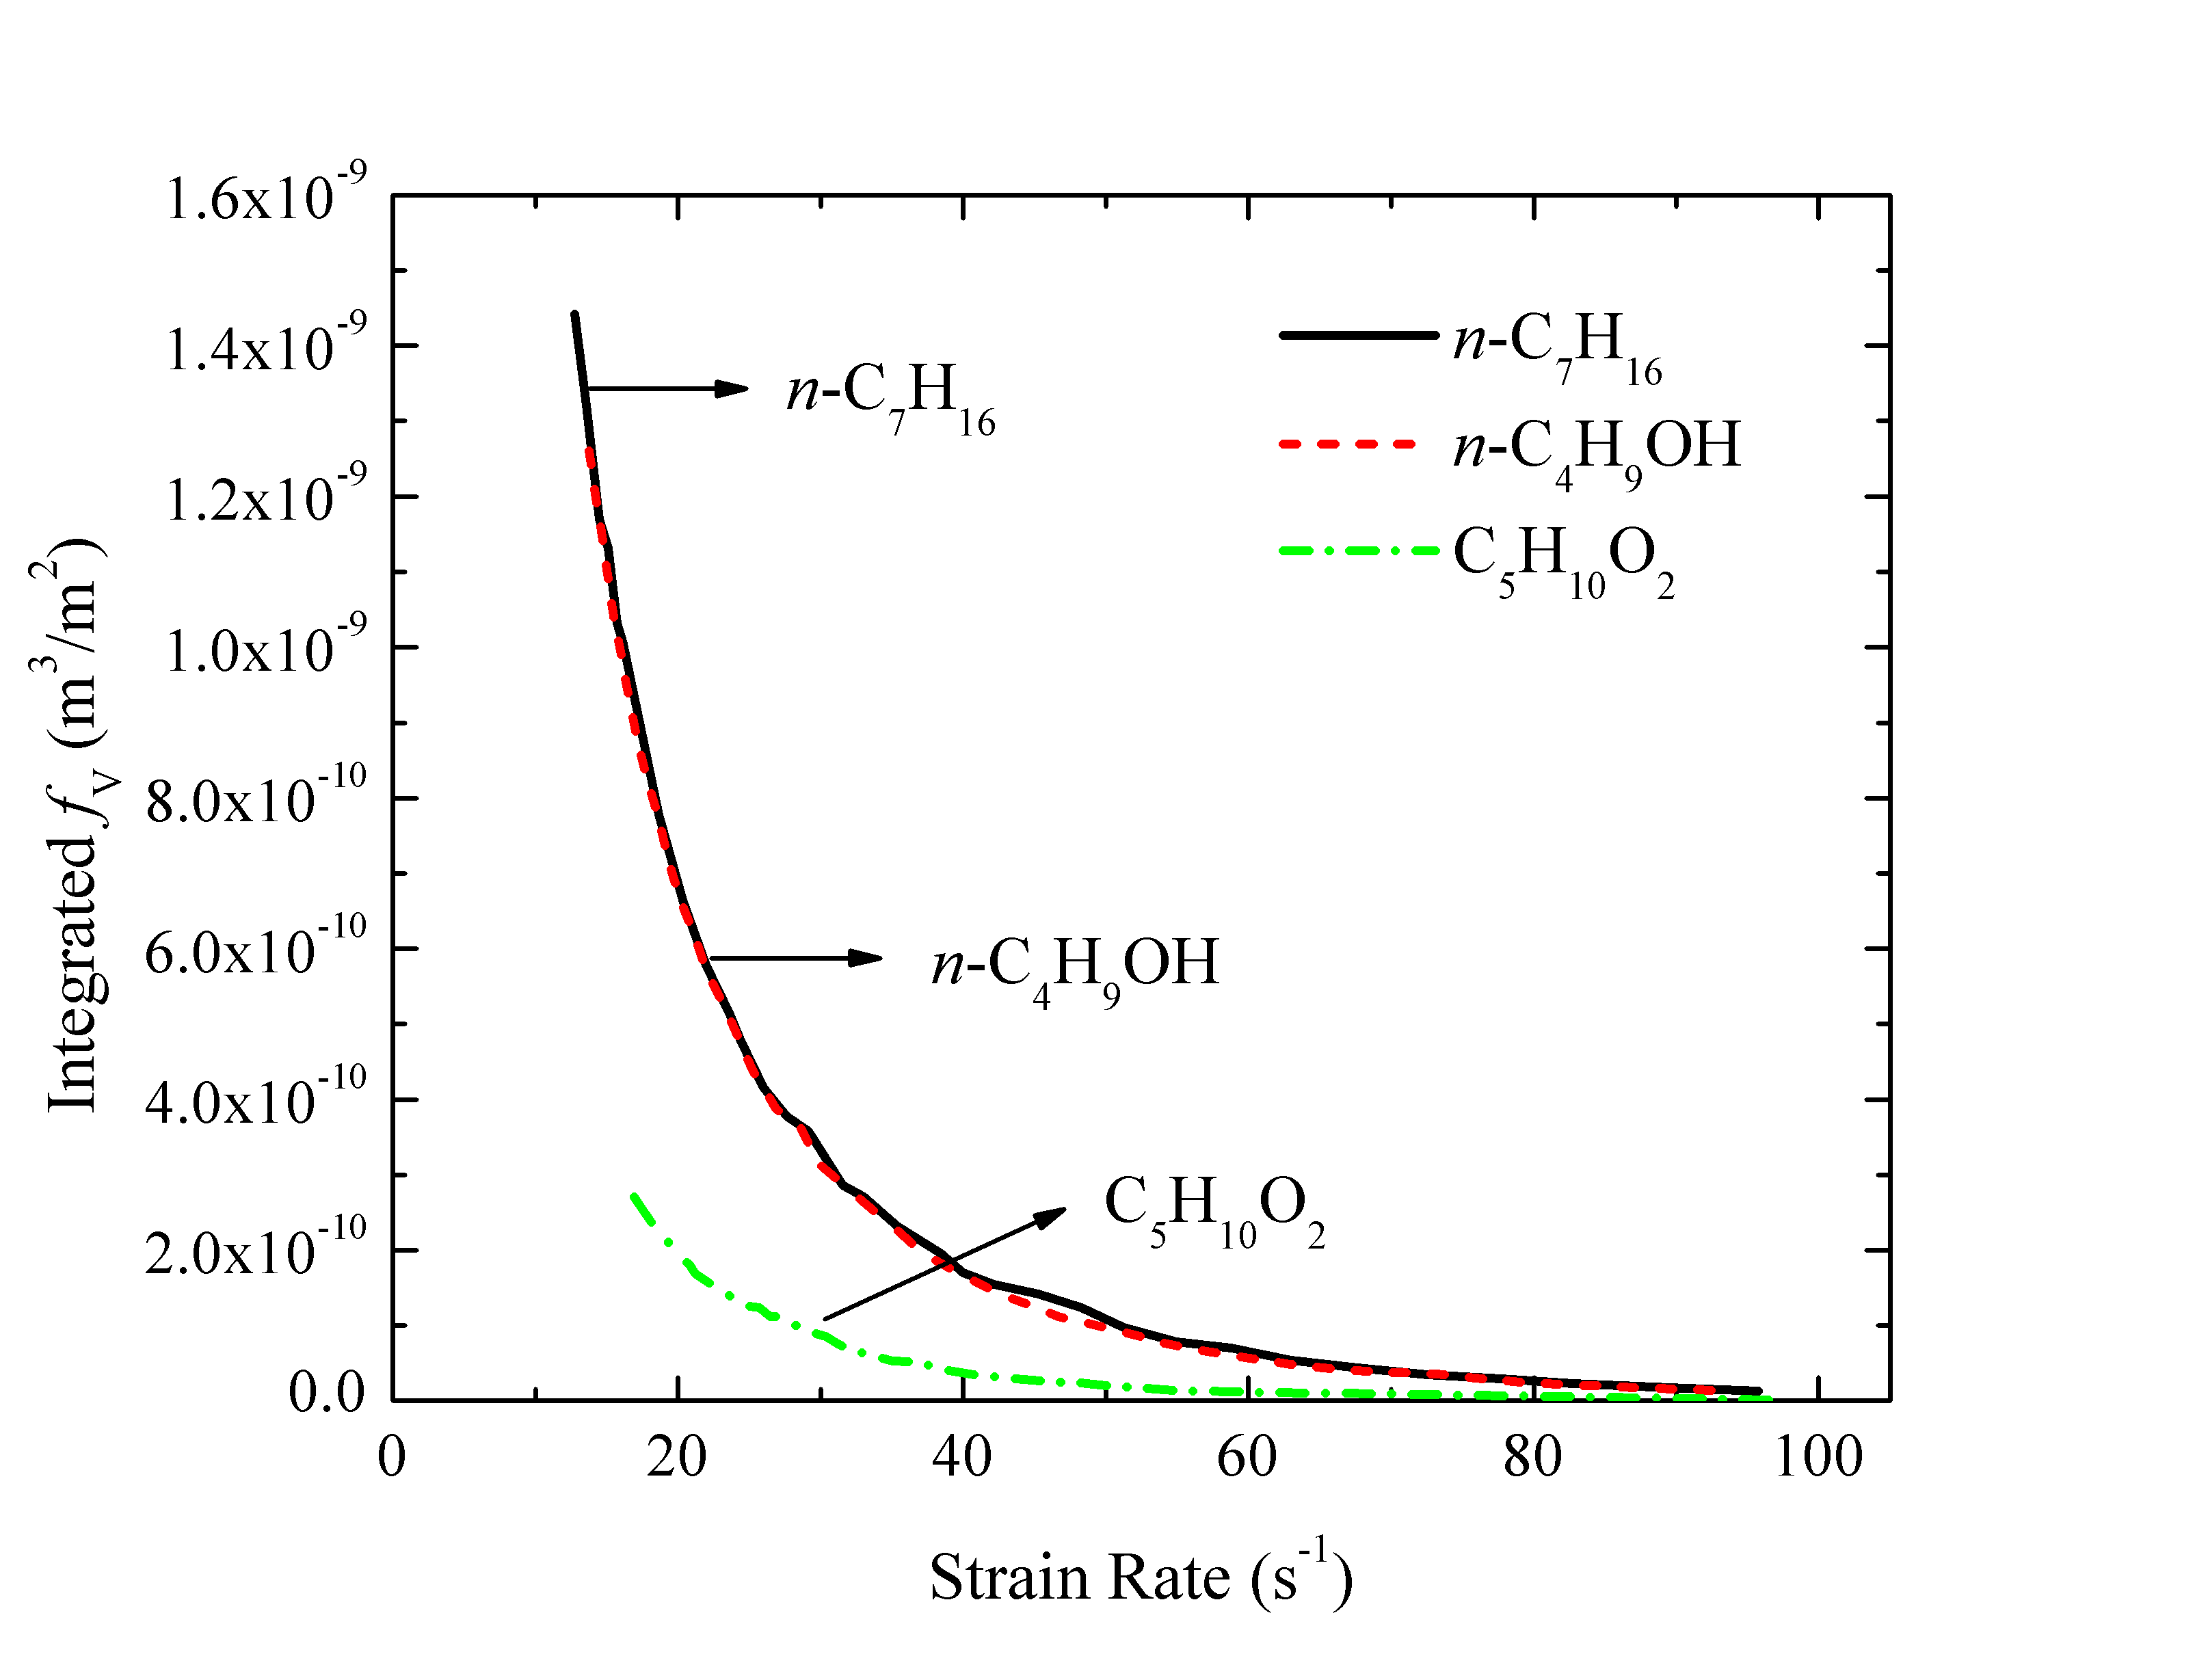
\includegraphics[trim=4mm 8mm 30mm 20mm, clip=true, width=0.48\textwidth]{SV-SR.png}
%  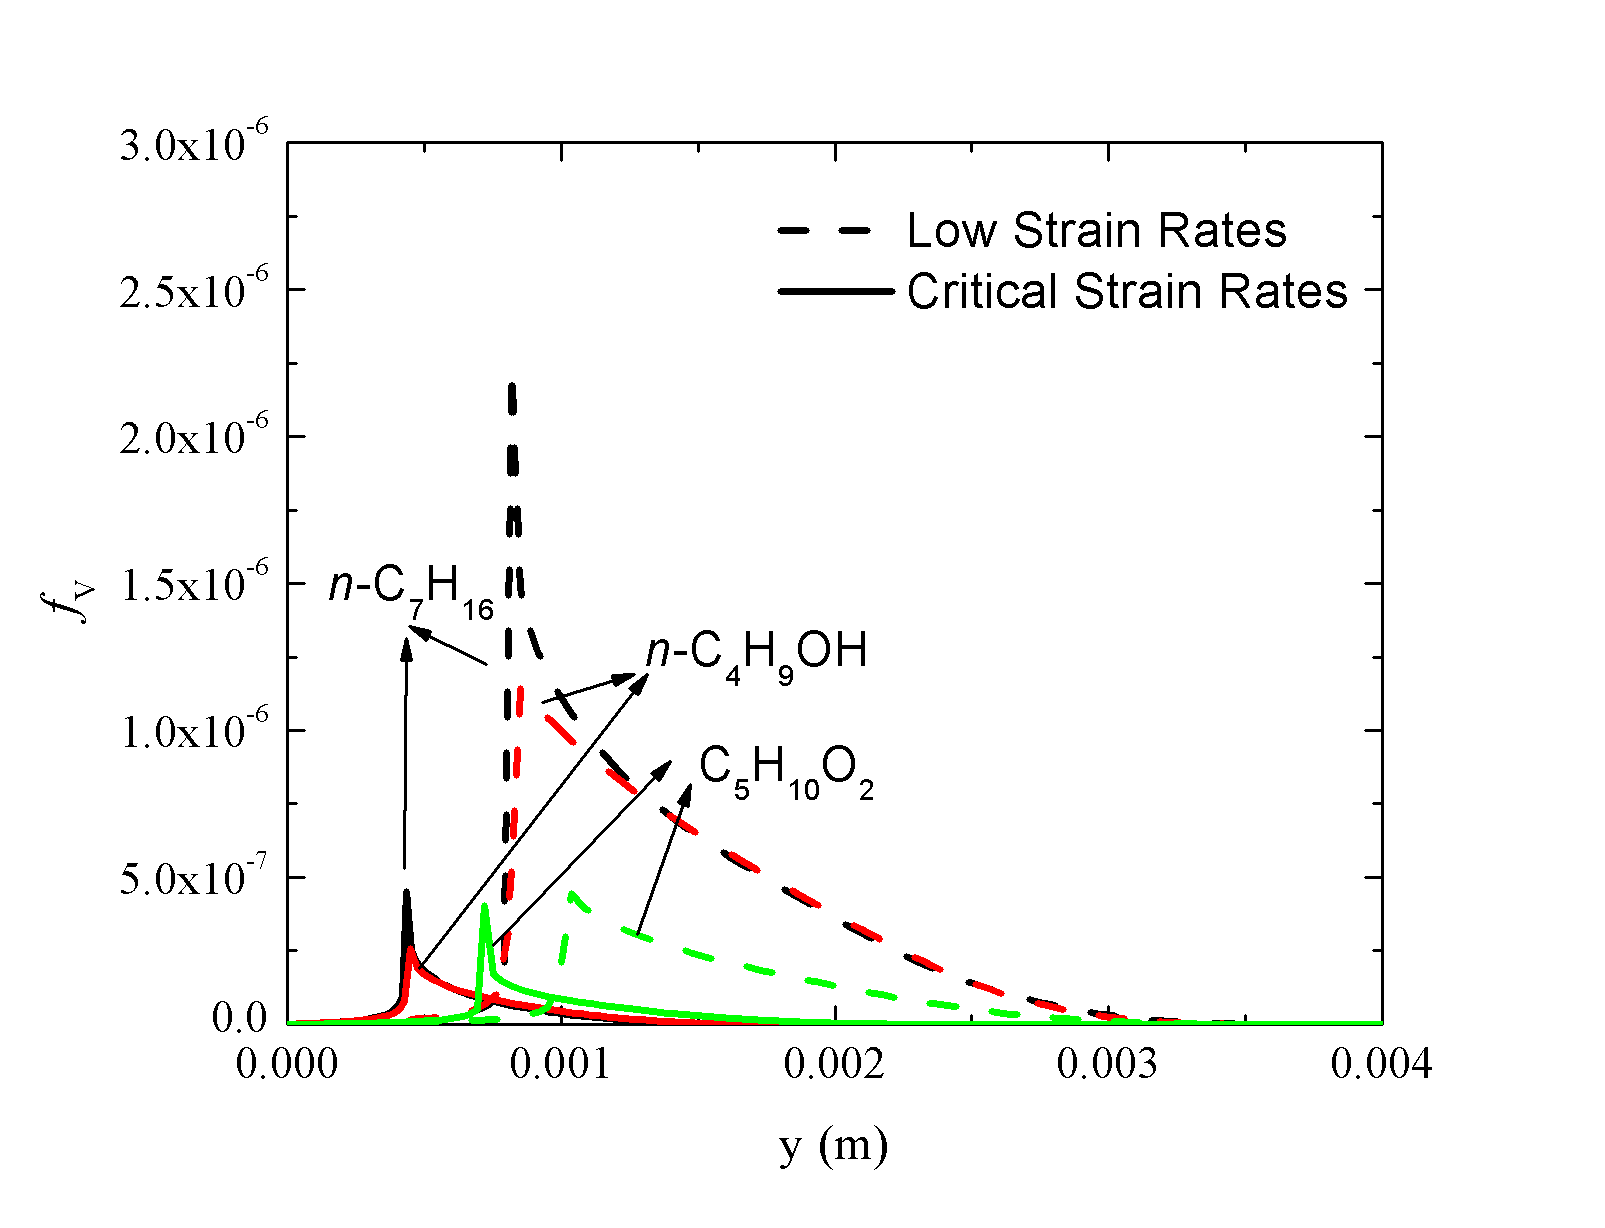
\includegraphics[trim=4mm 8mm 30mm 20mm, clip=true, width=0.48\textwidth]{fv-y.png}
%  \normalsize
%  \vspace{-0.2in}
%  \caption{The responses of $f_V$ to strain rates at $X_{O_2}=0.2$. Left: $f_V$ integrated along the center axis of the stagnation-flow field. Right: $f_V$ profiles at low strain rates ($16$ s$^{-1}$) and CSRs.}
%  \label{fig:fv-SR-combo}
%\end{figure*}

\subsection{Rate-Limiting Steps for PAH Formation}

To elucidate the rate-limiting step, profiles of soot precursors at low and critical strain rates are shown in Fig.~\ref{fig:CxHy}. All profiles shift in the direction of the liquid pool at higher flow rates as increased strain rates push the stagnation plane towards the pool. Species with ring structures, specifically C$_5$H$_6$ and C$_6$H$_6$ have lower concentrations at CSR, responding to strain similar to $f_V$. However, the upstream C$_3$ precursors, A-C$_3$H$_5$ and C$_3$H$_3$, have higher concentrations at CSR. Other upstream species such as C$_2$H$_2$ and C$_2$H$_4$ do not show significant difference.  This indicates that A-C$_3$H$_5$ and C$_3$H$_3$ species have insufficient residence times to form rings, resulting in the observed decrease in soot. Therefore, the ring formation reactions
\begin{align*}
  {\rm C}_2{\rm H}_2 + {\rm A}-{\rm C}_3{\rm H}_5 &\Longleftrightarrow {\rm H} + {\rm C}_5{\rm H}_6\\
  2 {\rm C}_3{\rm H}_3 &\longrightarrow {\rm C}_6{\rm H}_6
\end{align*}
are the rate-limiting steps and are the same for all three fuels.


\begin{figure*}[t]
  \centering
  \scriptsize
%  \vspace{-0.4in}
%  \hspace{-0.4in}
%  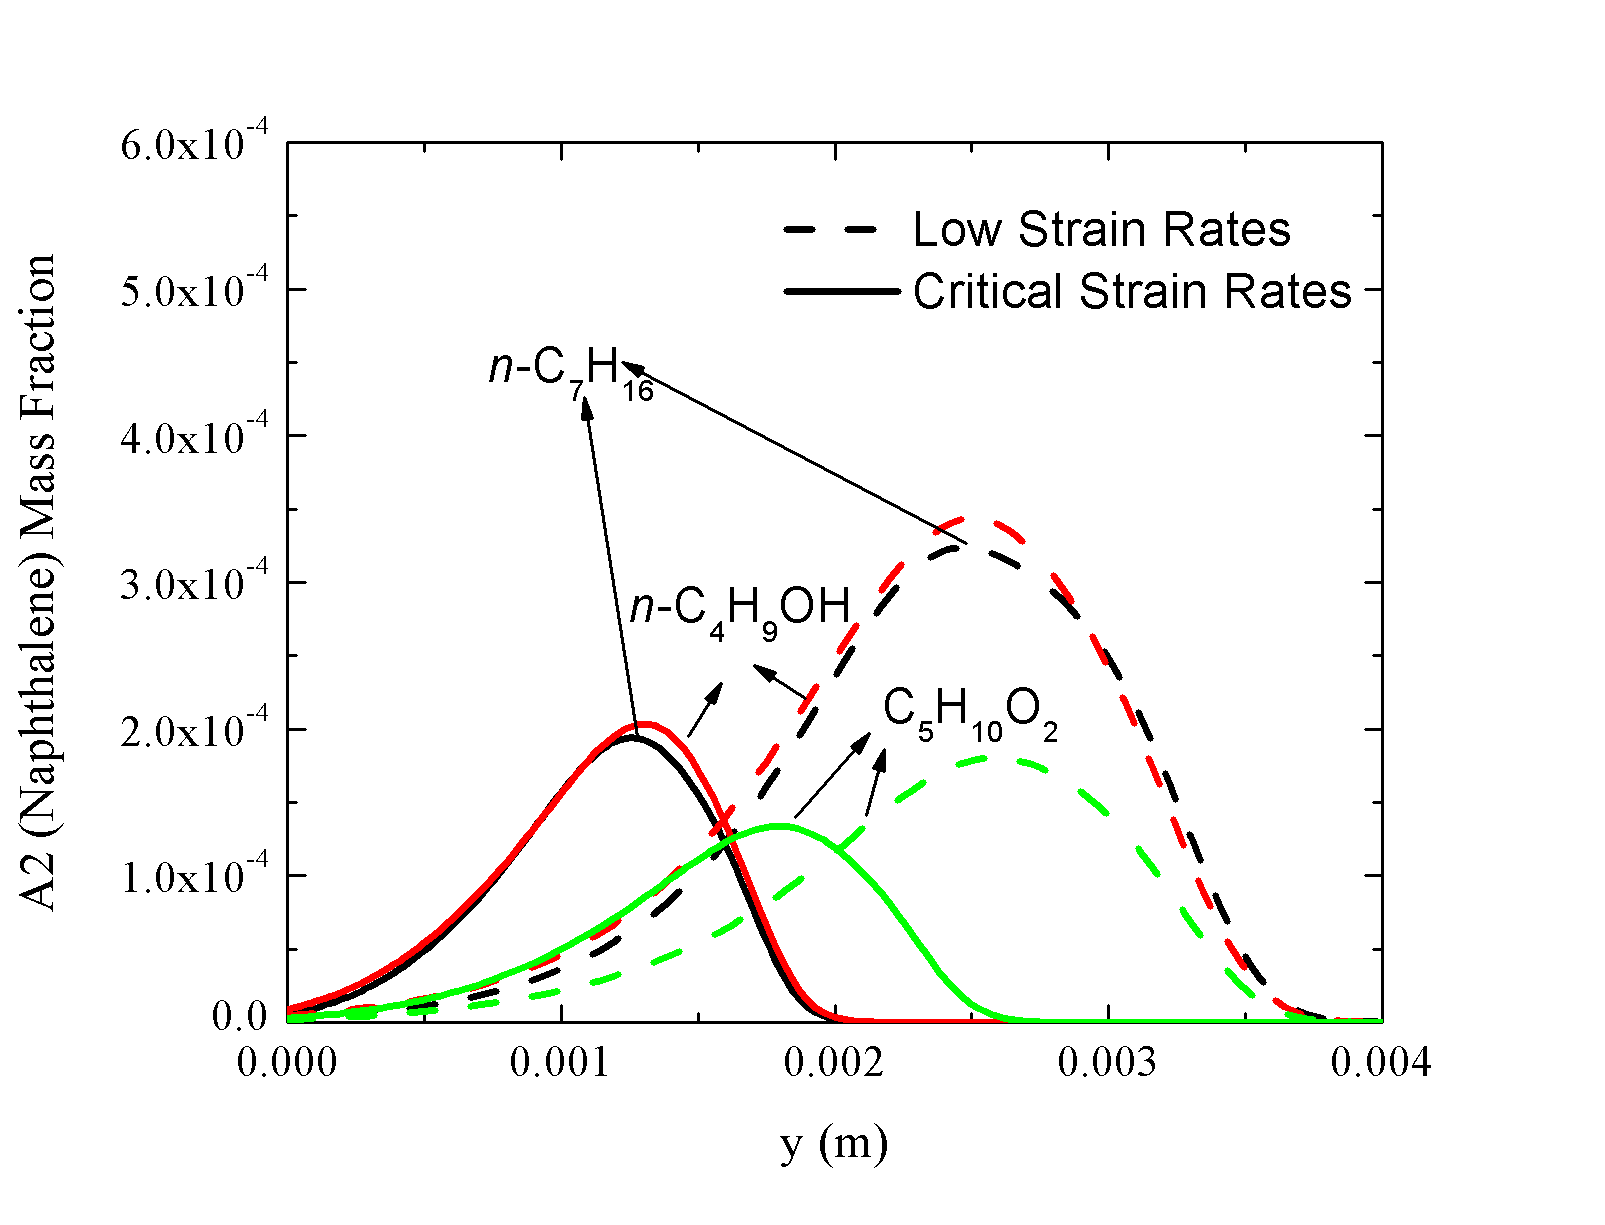
\includegraphics[trim=4mm 8mm 30mm 20mm, clip=true, width=0.48\textwidth]{A2-y.png}
%  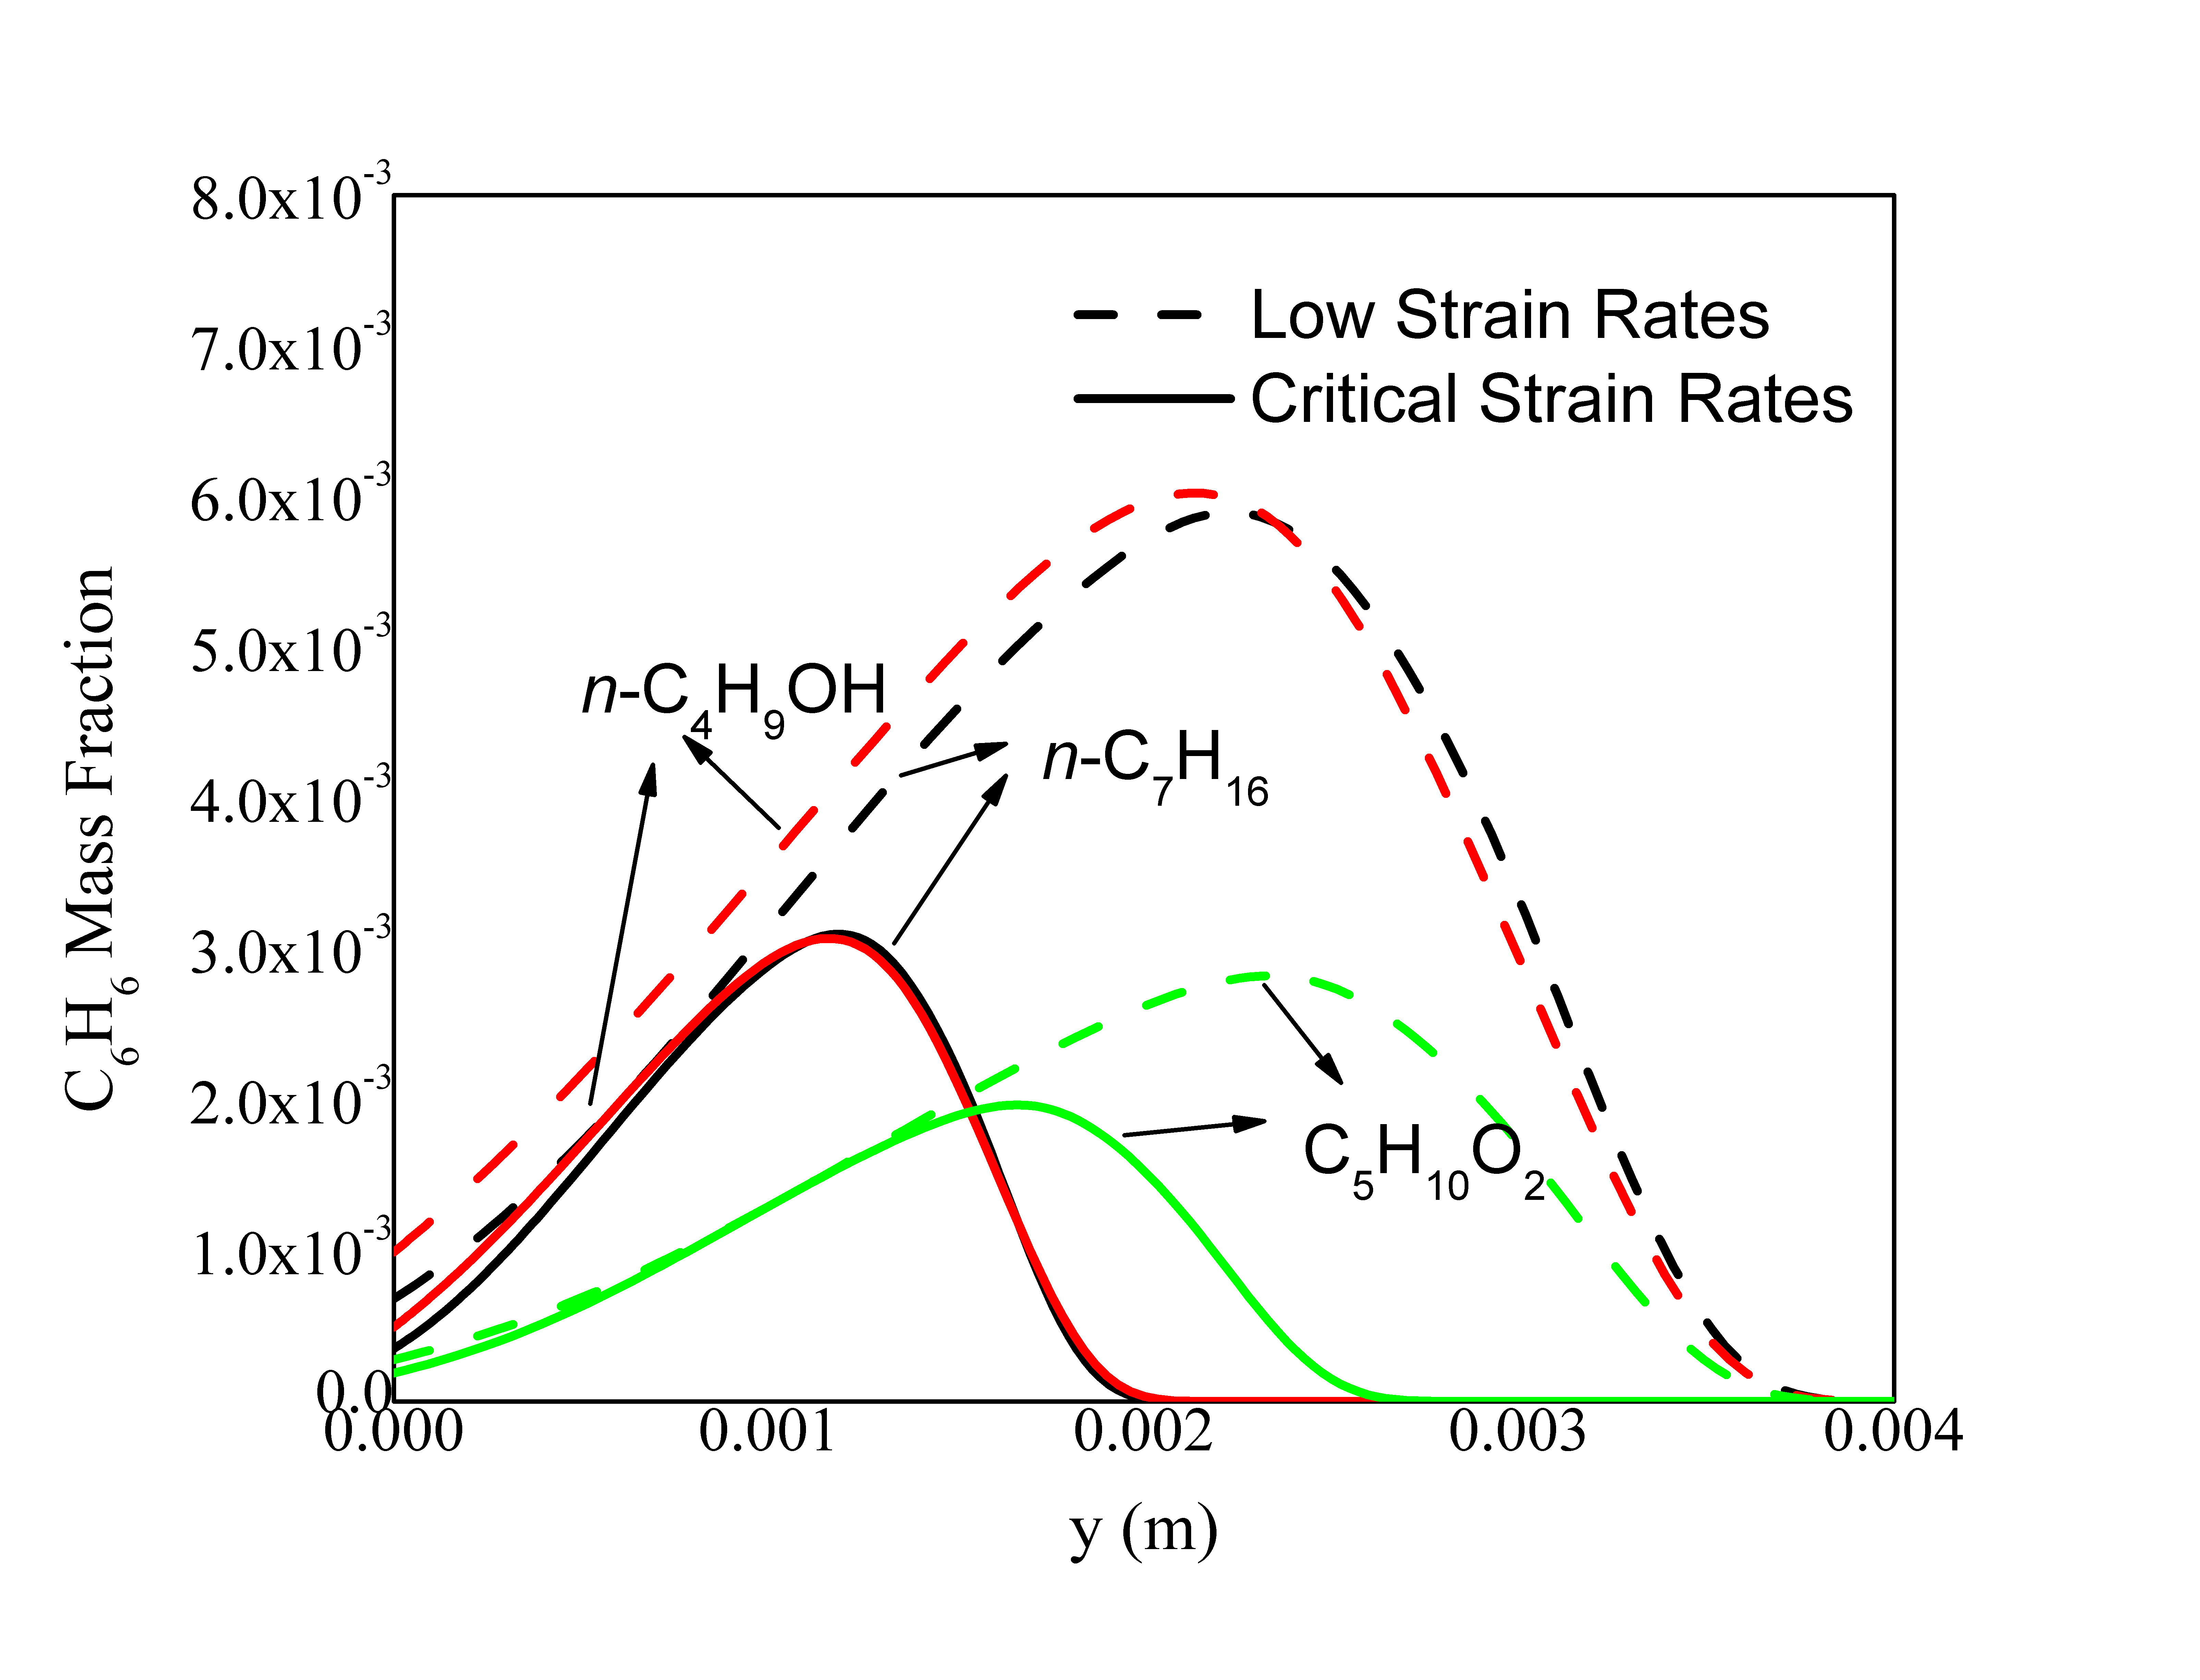
\includegraphics[trim=4mm 8mm 30mm 20mm, clip=true, width=0.48\textwidth]{A1-y.png}
%  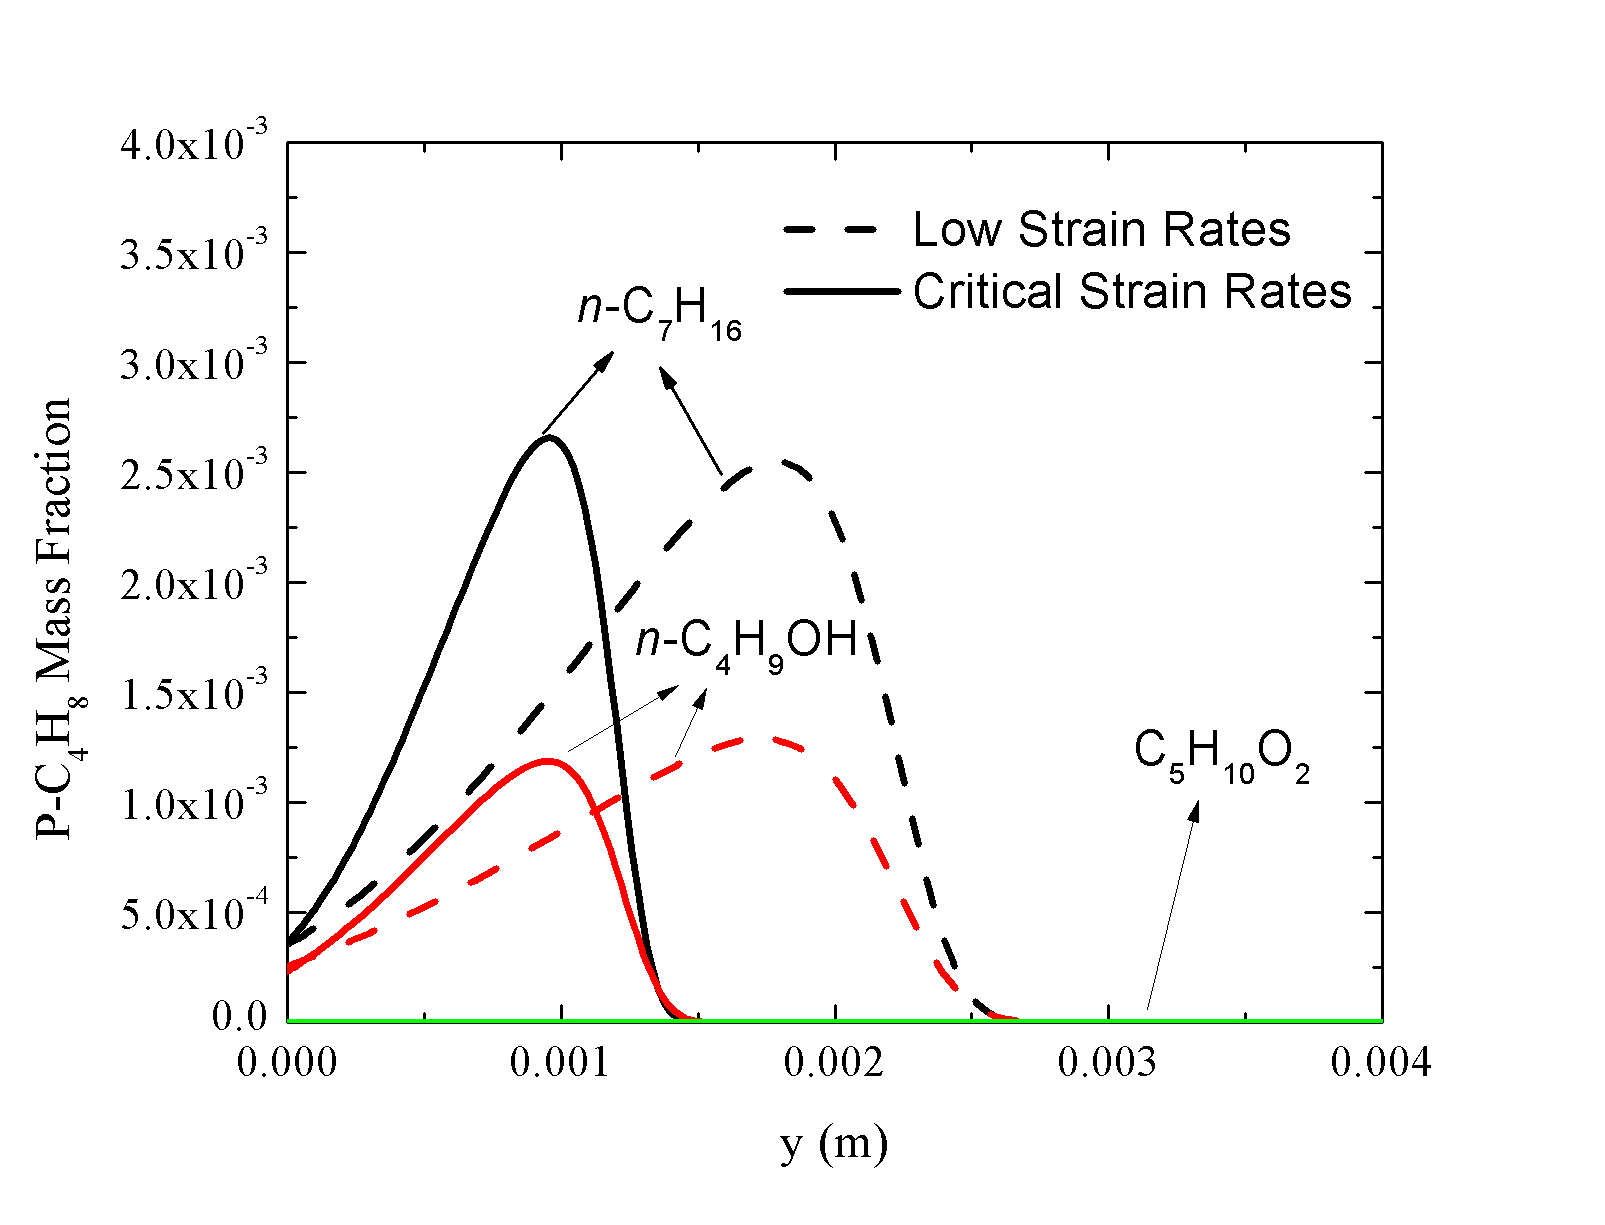
\includegraphics[trim=4mm 8mm 30mm 20mm, clip=true, width=0.48\textwidth]{P-C4H8-y.png}
%  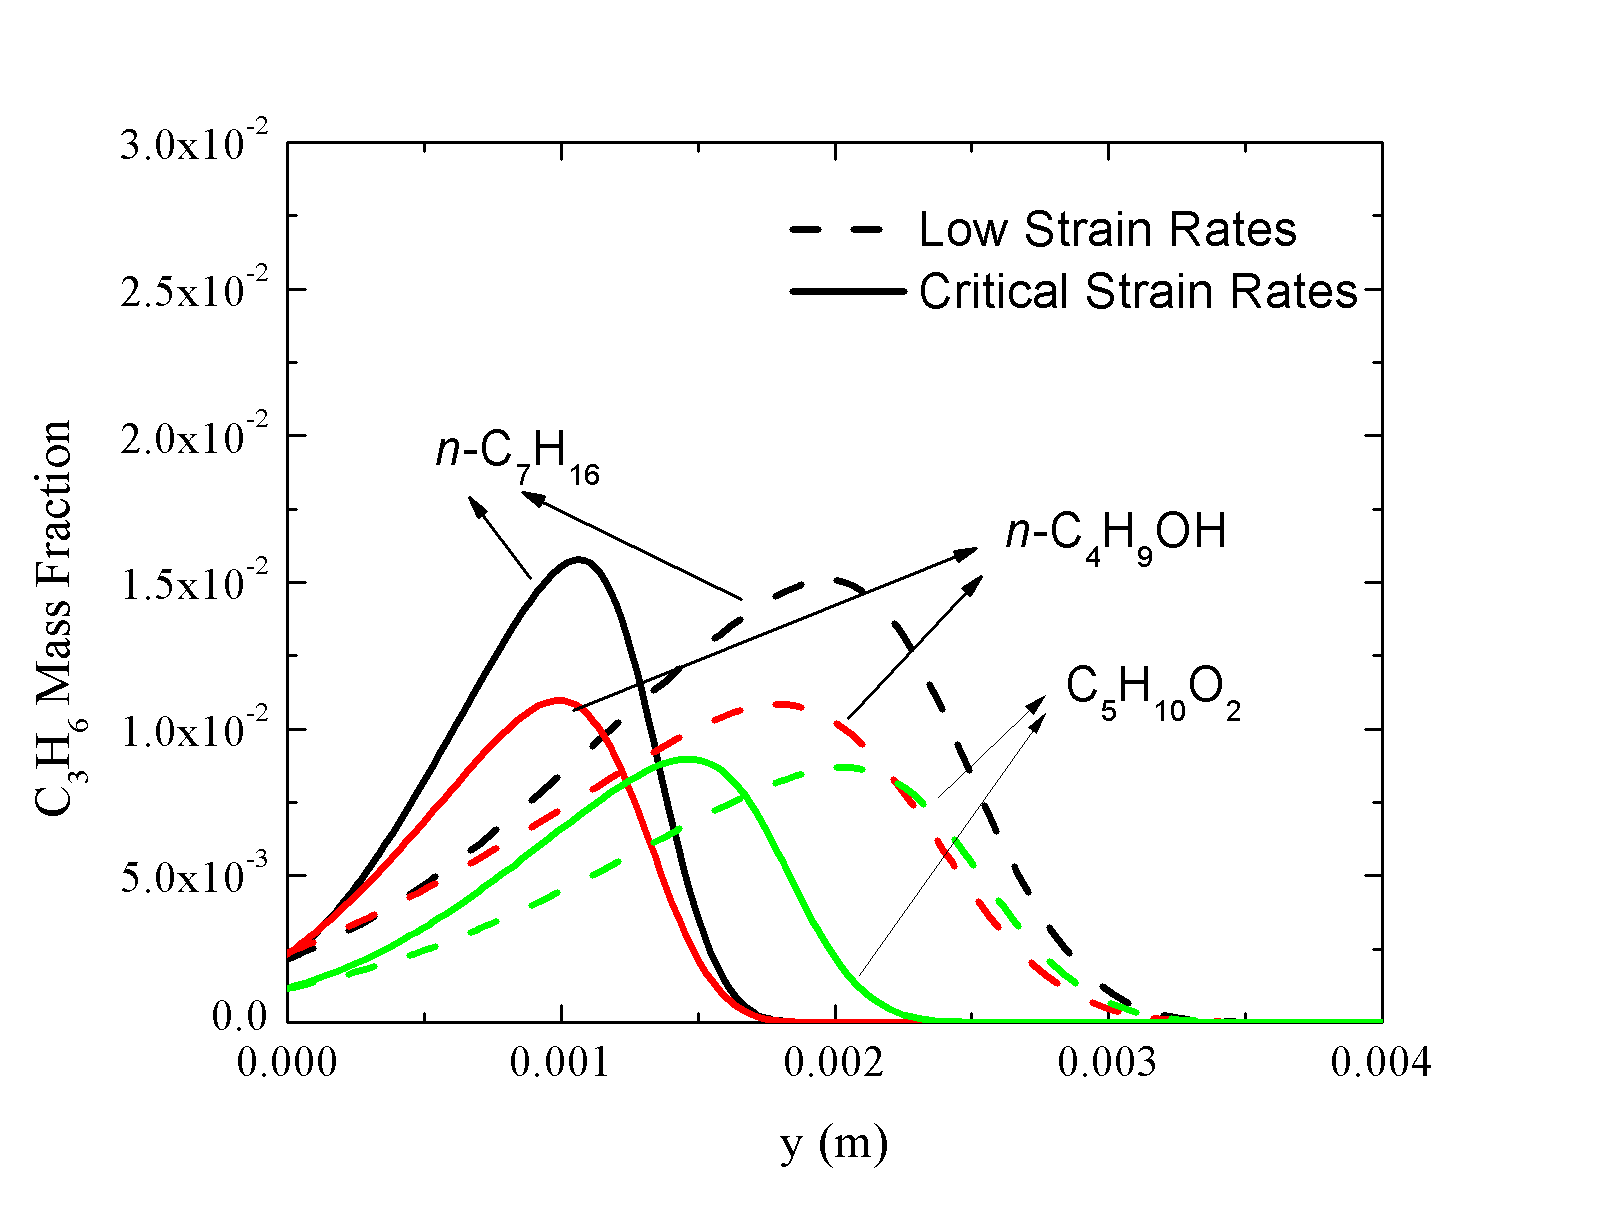
\includegraphics[trim=4mm 8mm 30mm 20mm, clip=true, width=0.48\textwidth]{C3H6-y.png}
  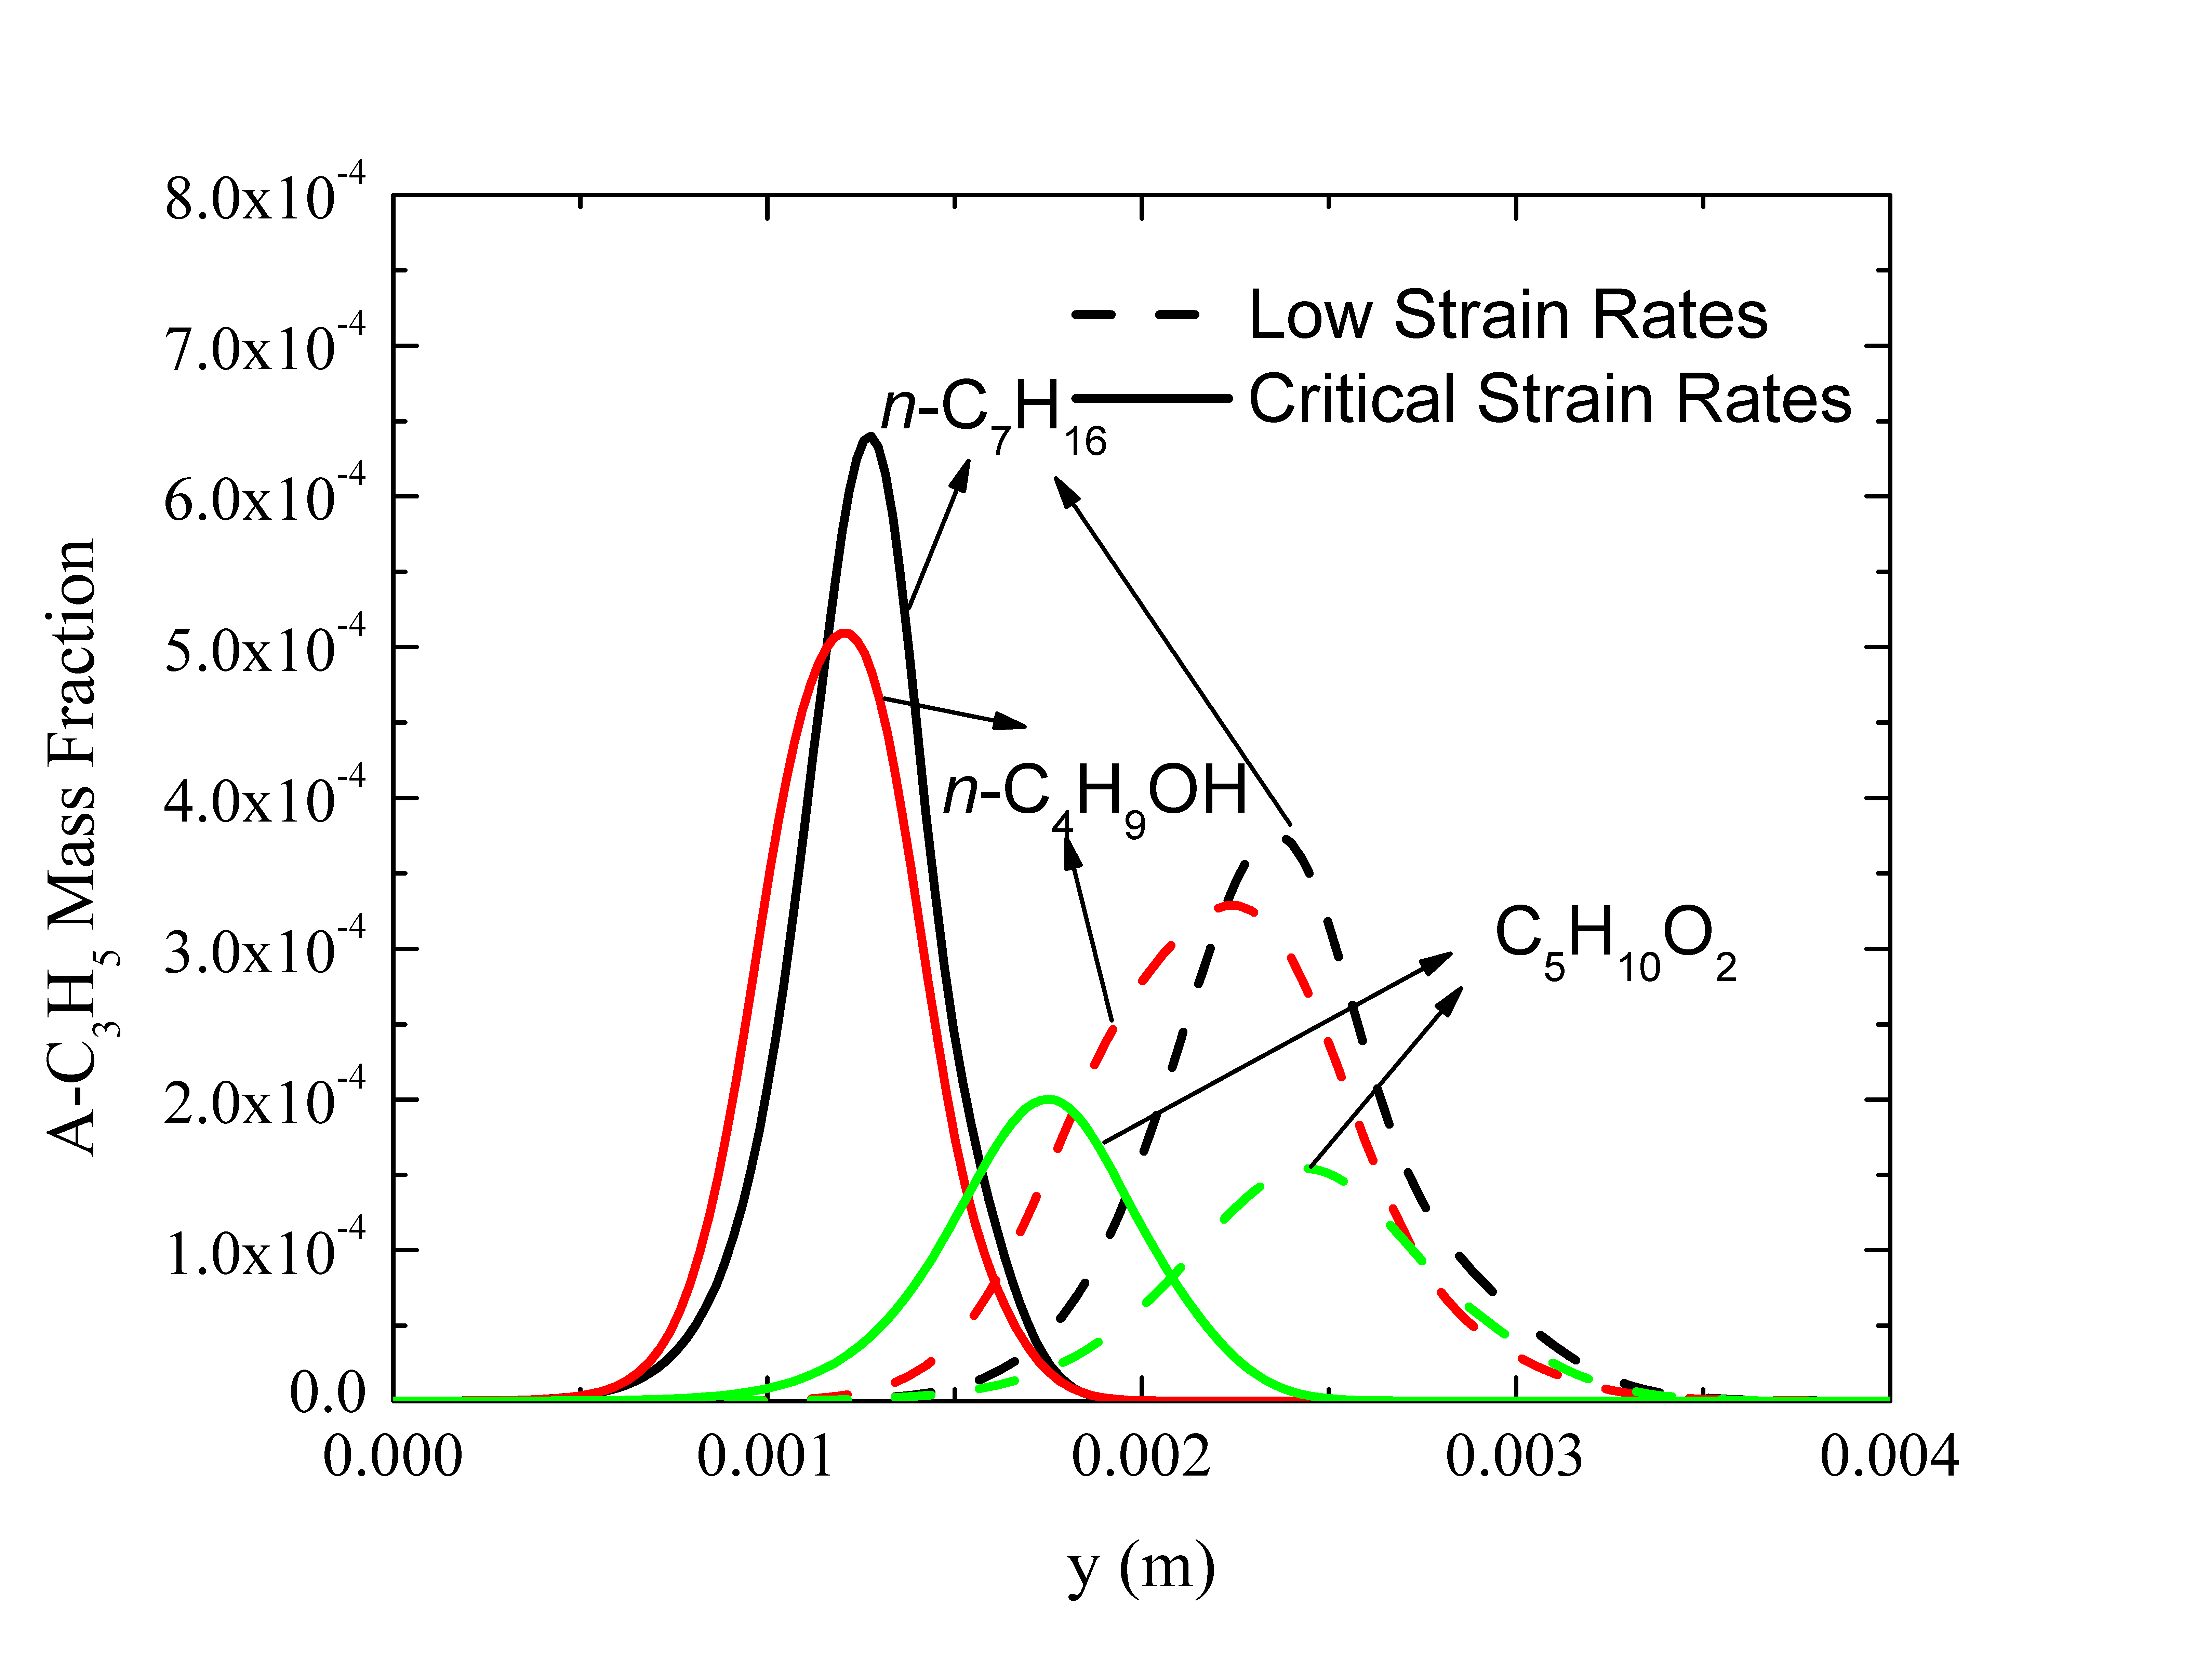
\includegraphics[trim=4mm 8mm 30mm 20mm, clip=true, width=0.4\textwidth]{A-C3H5-y.png}
  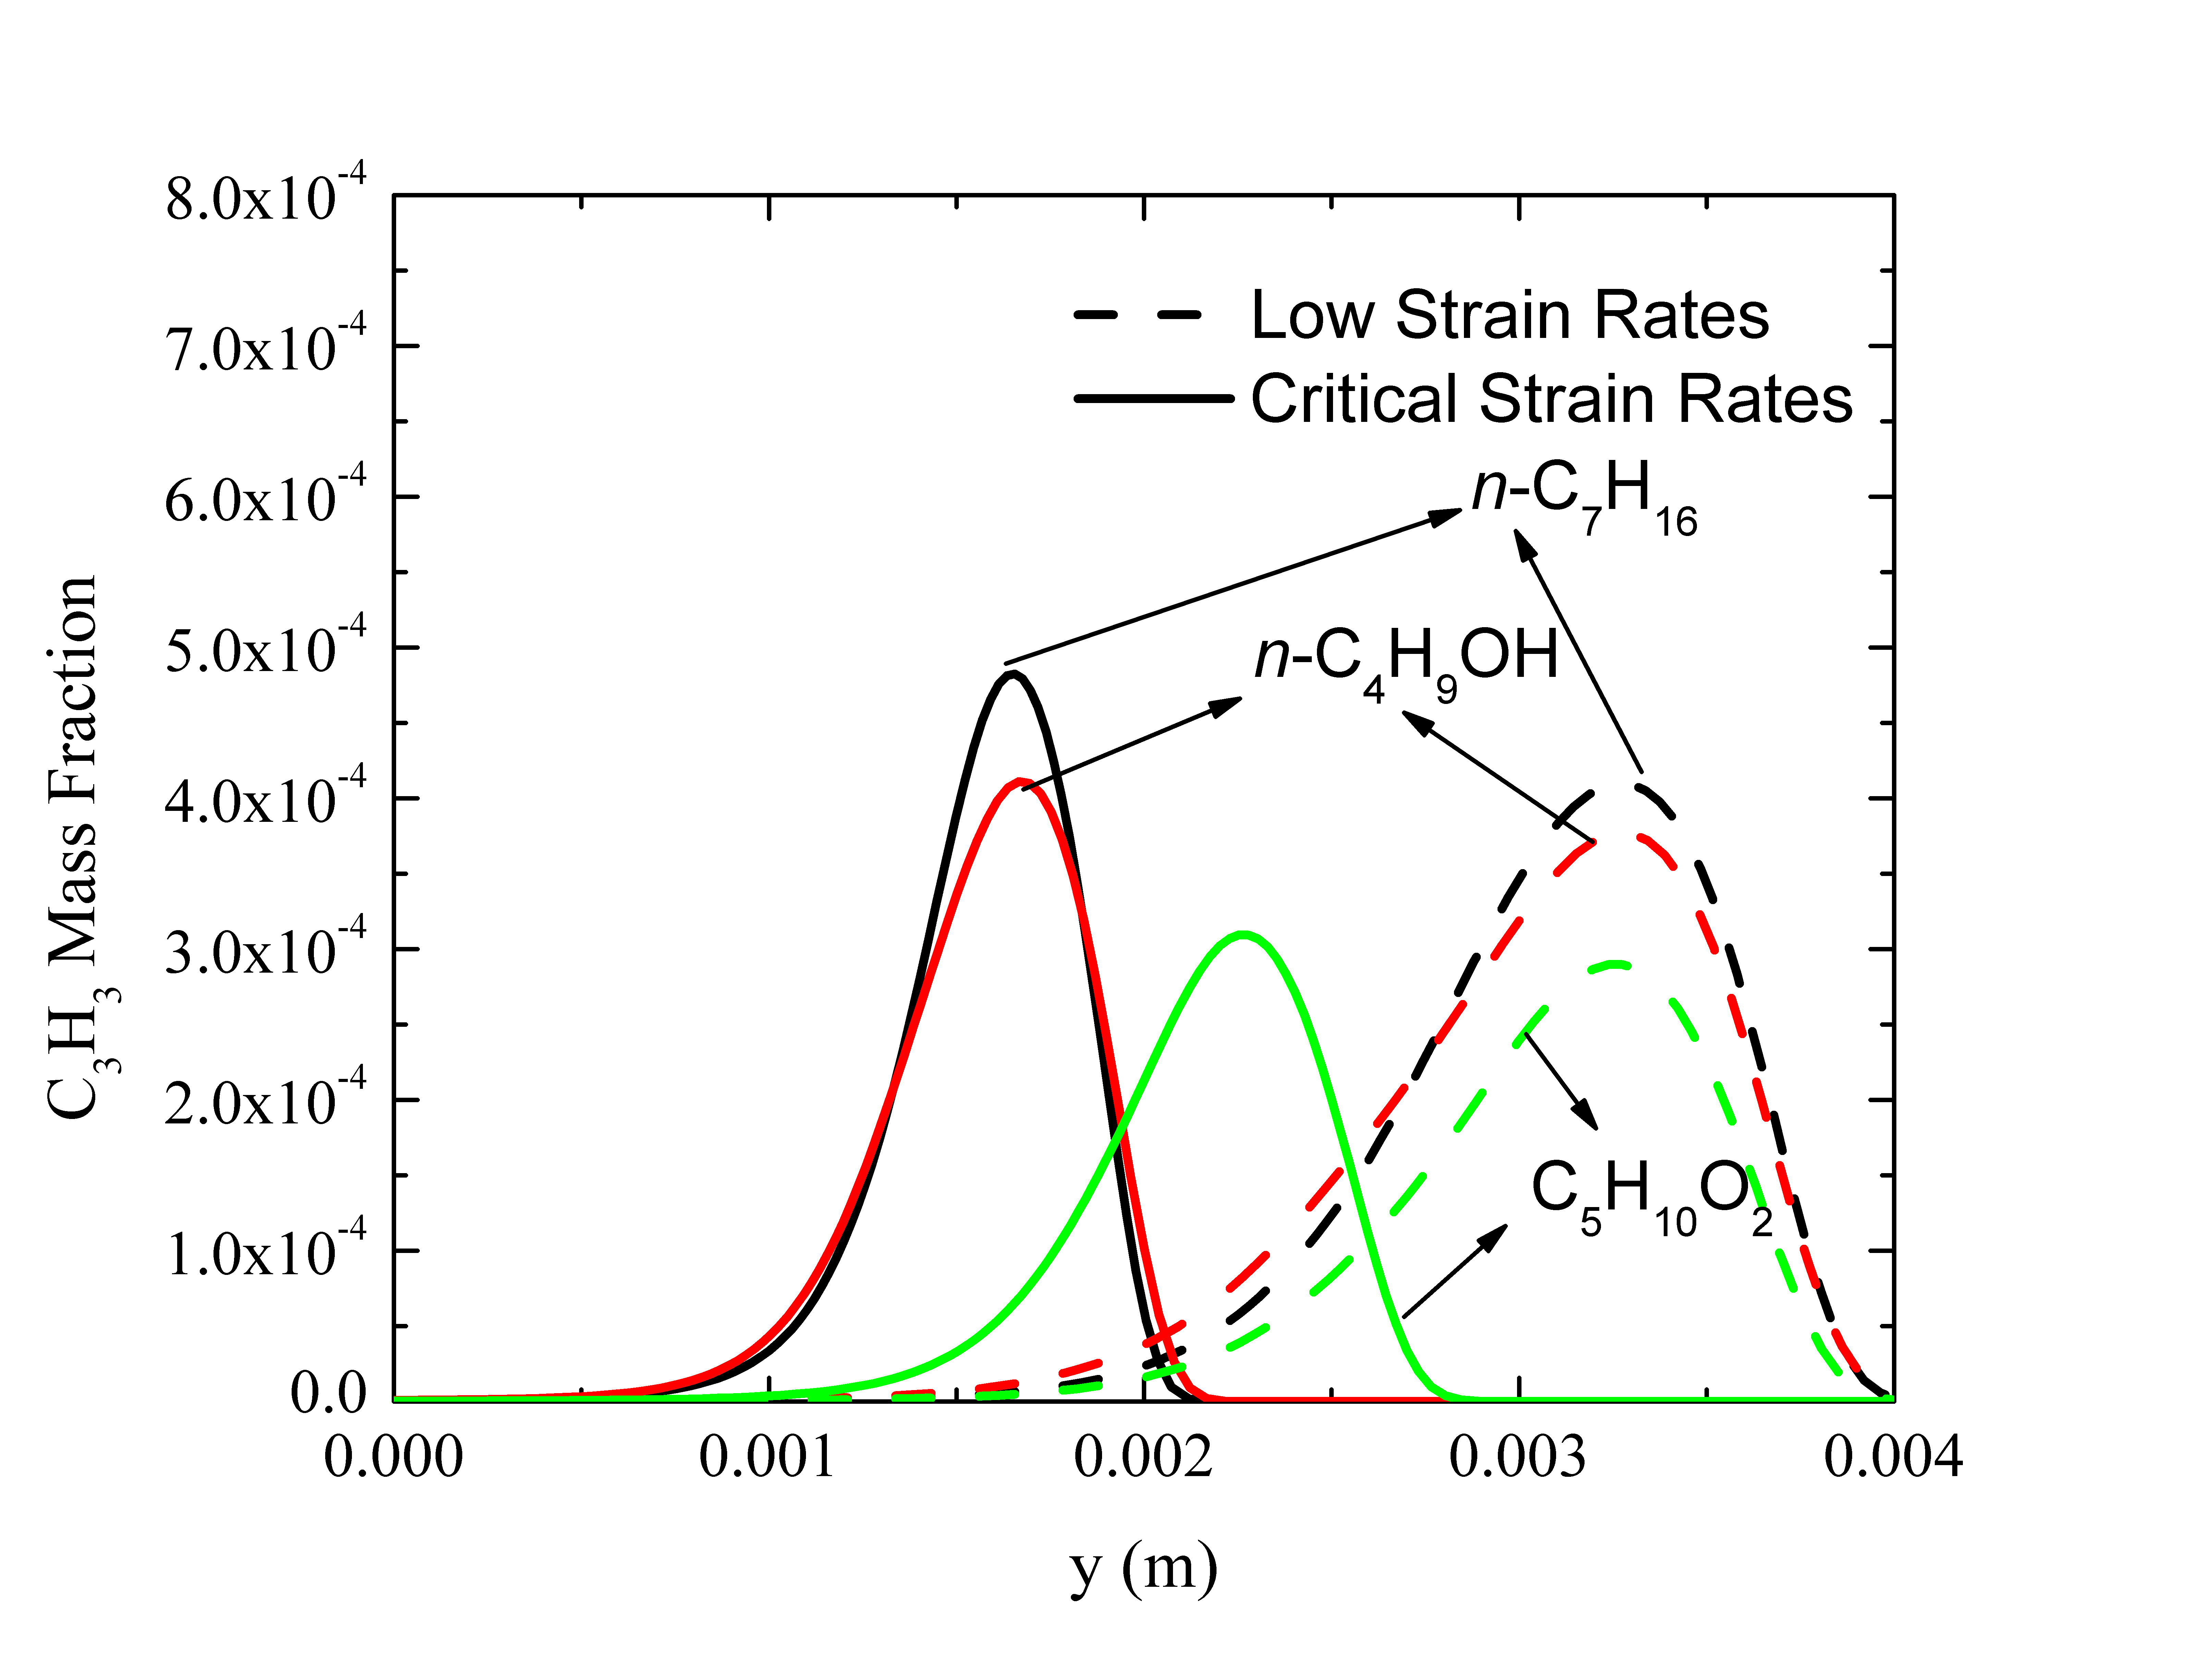
\includegraphics[trim=4mm 8mm 30mm 20mm, clip=true, width=0.4\textwidth]{C3H3-y.png}
  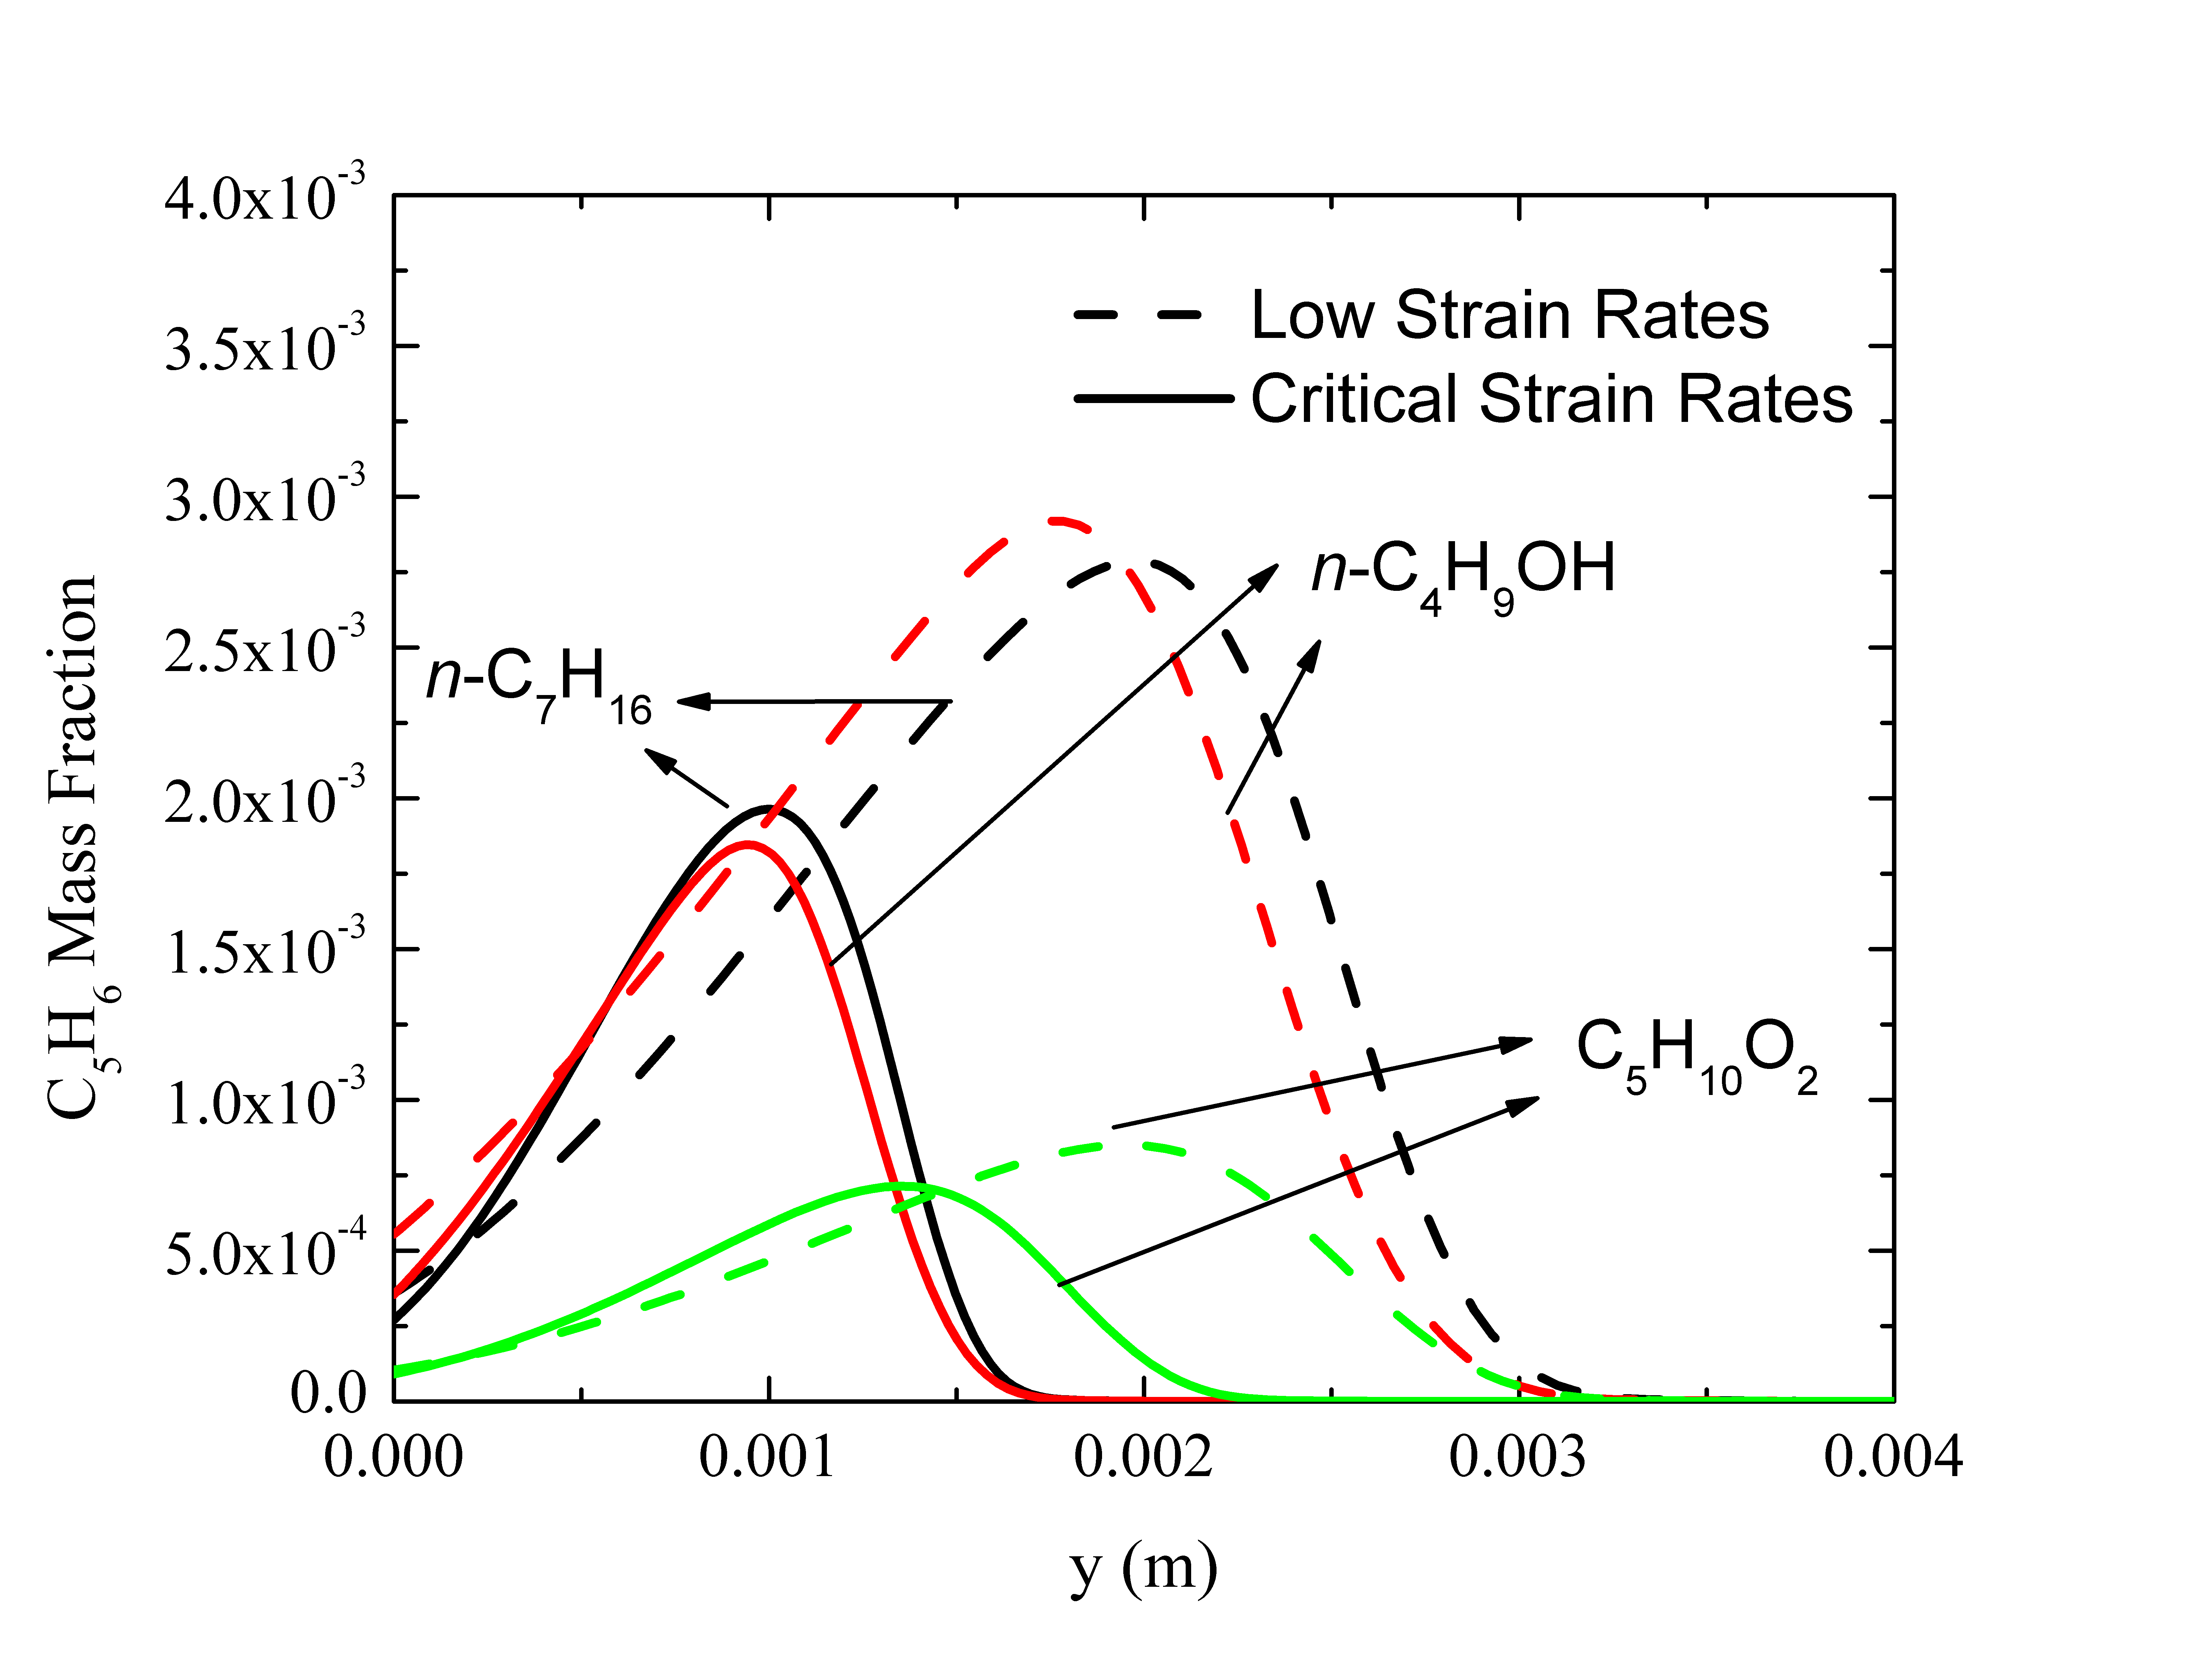
\includegraphics[trim=4mm 8mm 30mm 20mm, clip=true, width=0.4\textwidth]{C5H6-y.png}
  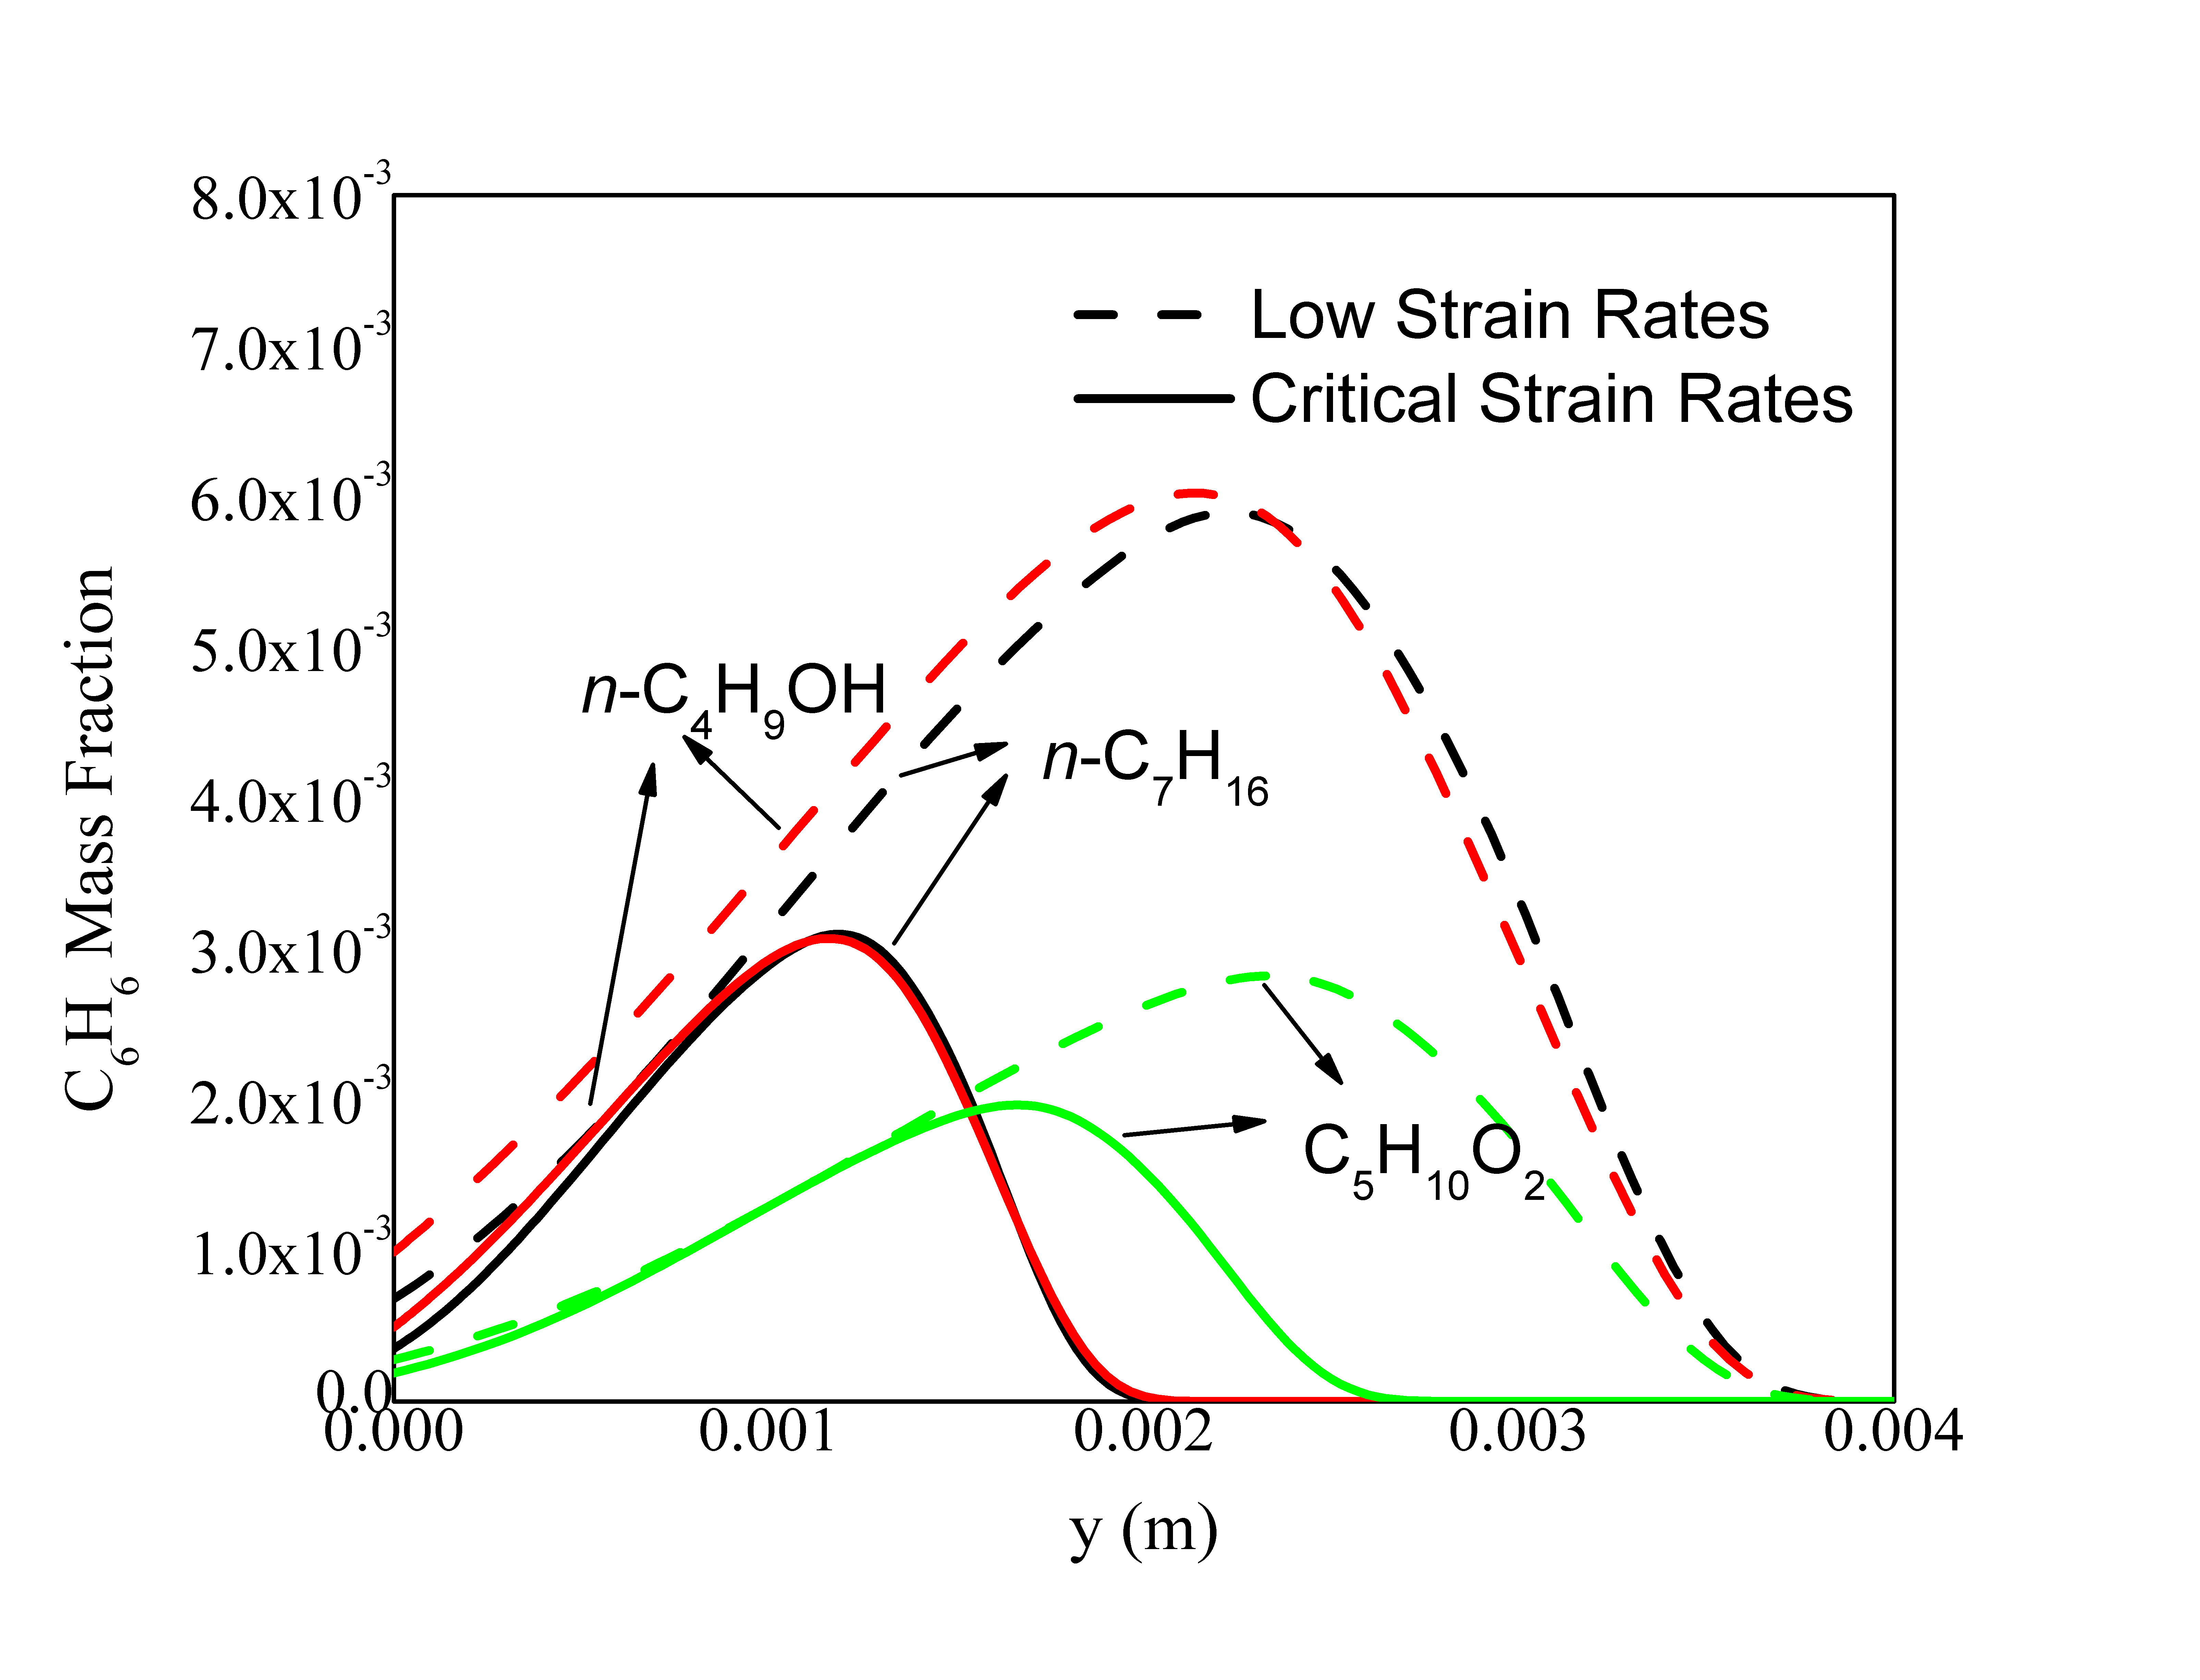
\includegraphics[trim=4mm 8mm 30mm 20mm, clip=true, width=0.4\textwidth]{A1-y.png}
  \normalsize
  \vspace{-0.1in}
  \caption{Key intermediate species profiles at low strain rates ($16$ s$^{-1}$) and CSRs: $X_{O_2}=0.2$.}
  \label{fig:CxHy}
\end{figure*}

\subsection{Summary}

Two hypotheses that might explain the lower CSRs of methyl butanoate compared to the other two fuels were proposed: if less soot is produced from methyl butanoate regardless of the strain rate and/or if soot formation reactions of methyl butanoate are more prone to extinction at reduced residence times.  The response of soot volume fraction to strain rate, chemical pathways for PAH formation, and the rate-limiting steps were examined to elucidate the relative roles of these two hypotheses.  Methyl butanoate is found to be significantly less sooting than $n$-heptane and $n$-butanol at all strain rates.  As the three fuels share similar PAH pathways, the fuel specific breakdown processes account for the different $f_V$ at the same strain rate.  Furthermore, the rate-limiting steps for all three fuels were identified and found the same.  Therefore, the difference in CSRs for three fuels are due to the total amount of soot formed with the three fuels, due to the difference in fuel breakdown processes that generate soot precursors.



\section{Conclusions}           

In this work, $n$-heptane, $n$-butanol, and methyl butanoate were chosen as diesel, bioalcohol, and biodiesel surrogates of interest due to their similar volatilities and consequent potential applications in diesel fuel blending. Their sooting limits were measured experimentally with the stagnation-flow apparatus. Computations were conducted for the same configuration using detailed PAH chemistry and a detailed soot model based on the Hybrid Method of Moments (HMOM). Argon dilution was adopted to keep the thermal environment for the three fuel cases essentially the same in order to elucidate the chemical effects.  Both experimental and computational results showed the critical strain rates of the three fuels, based on the absolute soot volume fraction, increase with increasing oxygen mole fraction in the oxidizer, due to the thermal effect. Moreover, although $n$-heptane and $n$-butanol show similar sooting propensities, methyl butanoate produces significantly less soot.

Sensitivity and reaction path analysis was performed for naphthalene, the first PAH species from which soot forms. This analysis revealed that, despite different sooting tendencies, the three fuels shared similar PAH chemical pathways. C$_5$, C$_6$, C$_7$ and C$_9$ rings as well as naphthalene are formed sequentially through the combination of C$_3$ and smaller chain radicals resulting from fuel cracking processes. Due to the fuel bound oxygen in methyl butanoate, less and shorter chain radicals are available for soot formation, compared with the other fuels, such that methyl butanoate forms the least soot and has the lowest critical strain rates.

The strain rate effects on soot formation were also examined. Despite different sooting propensities, for all three fuels, C$_5$ and C$_6$ ring formation reactions are the rate-limiting steps. Their concentrations drop as the residence time is reduced, such that the downstream PAH chemistry is consequently inhibited, resulting in the sooting limits.


\section*{Acknowledgments}
This work was supported by the Combustion Energy Frontier Research Center, an Energy Frontier Research Center funded by the US Department of Energy, Office of Basic Energy Sciences under Award Number DE-SC0001198.

\section*{References}
\bibliographystyle{elsarticle-num-CNF}
\bibliography{Soot_m}


\renewcommand{\thefigure}{\arabic{figure}}
\renewcommand{\thetable}{\arabic{table}}

\end{document}

